%=======================================================================
%
% ------------------------------------------------------------------------
% ------------------------------------------------------------------------
% abnTeX2: Modelo de Trabalho Academico  em conformidade com 
% ABNT NBR 14724:2011: Informacao e documentacao - Trabalhos academicos
% ------------------------------------------------------------------------
%Customização IFC
% ------------------------------------------------------------------------
% Autor:  Tiago Possato (tiago.possato@yahoo.com.br), baseado no modelo de Eliton Tiago (elitontiago@hotmail.com)
% Adaptação: Fábio Pinheiro (fabio.pinheiro@ifc.edu.br)
% Versão: 16 de abril de 2024.
% Codificação: UTF-8
% LaTeX:  abnTeX2
%
%=======================================================================

\documentclass[
	% -- opções da classe memoir --
	12pt,				% tamanho da fonte	
	oneside,          % não imprimir em verso e anverso, oposto do twoside 
	a4paper,			% tamanho do papel. 
	% -- opções da classe abntex2 --
	chapter=TITLE,		% títulos de capítulos convertidos em letras maiúsculas
	section=TITLE,		% títulos de seções convertidos em letras maiúsculas
	subsection=TITLE,	% títulos de subseções convertidos em letras maiúsculas
	%subsubsection=TITLE,% títulos de subsubseções convertidos em letras maiúsculas
	% -- opções do pacote babel --
	english,			% idioma adicional para hifenização
	brazil			% o último idioma é o principal do documento
	,sumario=tradicional,
	]{abntex2-IFC}


% ---
% Pacotes fundamentais 
% ---




%\begin{document}
\usepackage{float}
\usepackage{cmap}				% Mapear caracteres especiais no PDF
\usepackage{times}			    % Usa a fonte Times
\usepackage[T1]{fontenc}		% Selecao de codigos de fonte.fontenc
\usepackage[utf8]{inputenc}		% Codificacao do documento (conversão automática dos acentos)
\usepackage{lastpage}			% Usado pela Ficha catalográfica
\usepackage{indentfirst}		% Indenta o primeiro parágrafo de cada seção.
\usepackage{color}				% Controle das cores
\usepackage{graphicx}			% Inclusão de gráficos
\usepackage{amsfonts}			% Símbolos

\usepackage{longtable}
%\usepackage{geometry}
%\geometry{a4paper, margin=2.5cm}
\usepackage{array}
\renewcommand{\arraystretch}{1.2}

%----Ajuste no alinhamento das listas
\usepackage{enumitem}
\setitemize[0]{itemindent=0.4cm,itemsep=0pt}
\setenumerate[0]{itemindent=0.5cm,itemsep=0pt}
%------
% ---
% Pacotes de citações
% ---
\usepackage[brazilian,hyperpageref]{backref}	 					  % Paginas com as citações na bibl

%% Comentários do professor
\usepackage[textwidth=18mm,colorinlistoftodos,prependcaption,textsize=tiny]{todonotes}
\setlength{\marginparwidth}{19mm}

\usepackage{xargs} 
\newcommandx{\incerto}[2][1=]{\todo[linecolor=red,backgroundcolor=red!25,bordercolor=red,#1]{#2}}
\newcommandx{\alterar}[2][1=]{\todo[linecolor=blue,backgroundcolor=blue!25,bordercolor=blue,#1]{#2}}
\newcommandx{\info}[2][1=]{\todo[linecolor=green,backgroundcolor=green!25,bordercolor=green,#1]{#2}}
\newcommandx{\melhorar}[2][1=]{\todo[linecolor=yellow,backgroundcolor=yellow!25,bordercolor=yellow,#1]{#2}}
\usepackage{soul,color}
%Lista de Acronimos
\usepackage[acronym, nomain, nonumberlist]{glossaries}
%\usepackage{glossaries-extra}
\makeglossaries

\usepackage[a4paper]{geometry}
\geometry{a4paper, margin=2.5cm}
%Referência
\usepackage[alf, 	
			 		abnt-emphasize=bf,
				    abnt-url-package=none,
				    abnt-repeated-title-omit=yes,
				    abnt-full-initials=yes,                                        %yes nome por extenso, no apenas iniciais
					abnt-etal-list=3												%abreviar com mais de 3 autores
]{abntex2/abntex2cite}				 														    % Citações padrão ABNT
\usepackage{lipsum}							   								       % para geração de dummy text
\usepackage{multirow}
\usepackage{float}
\usepackage{setspace}
\usepackage{tabularx}

%\usepackage[none]{hyphenat}
%\captionsetup[table]{justification=raggedright}
% Configurações de aparência do PDF final
% alterando o aspecto da cor azul
\definecolor{blue}{RGB}{41,5,195}

% --- 
% Espaçamentos entre linhas e parágrafos 
% --- 
% O tamanho do parágrafo é dado por:
\setlength{\parindent}{2cm}
\linespread{1.5}

%Espaçamento depois dos títulos
\setlength{\afterchapskip}{\baselineskip}
% %\setlength{\afterchapskip}{\lineskip}

% Controle do espaçamento entre um parágrafo e outro:
\setlength{\parskip}{0cm}  % tente também \onelineskip

\hangcaption
\captionstyle[\raggedright]{}

%Estava mostrando nas referencias quais paginas estavam sendo referenciadas
\renewcommand{\backref}{}
\renewcommand*{\backrefalt}[4]{}

%Reduzir a fonte do caption
%\captionnamefont{\centering\ABNTEXfontereduzida}
%\captiontitlefont{\centering\ABNTEXfontereduzida}
%Ajuste nas listas de tabela, ilustrações e quadros
\setlength\cftbeforechapterskip{0pt}
% ---
% compila o indice
% ---
\makeindex
% ---


%----Include da capa agora está dentro do documento 
% ---
% Informações de dados para CAPA e FOLHA DE ROSTO
% ---

\titulo{\uppercase{desenvolvimento de uma ferramenta front-end para gerenciar retiros espirituais}}
\autor{\uppercase{Vitor Carlet}}
\local{Videira}
\data{2025}
\orientador[Orientador:]{TIAGO LOPES GONCALVES}
%\coorientador[Coorientador:]{professor coorientador}
\instituicao{ Ministério da Educação\\
        Secretaria de Educação Profissional e Tecnológica\\
        Instituto Federal Catarinense\\
        Campus Videira}
\tipotrabalho{Trabalho de Conclusão de Curso}
% O preambulo deve conter o tipo do trabalho, o objetivo, 
% o nome da instituição e a área de concentração
\preambulo{Projeto de Trabalho de Conclusão de Curso apresentado ao
Curso de graduação em Ciência da Computação do
Instituto Federal Catarinense – Campus Videira para
obtenção do título de bacharel em Ciência da Computação.

Orientador: \imprimirorientador}
% ---


%---


\begin{document}

% Retira espaço extra obsoleto entre as frases.

\frenchspacing 

% ----------------------------------------------------------
% ELEMENTOS PRÉ-TEXTUAIS
% ----------------------------------------------------------

%--- CAPA ----
\imprimircapa	% Capa do trabalho, deve ser preenchida à mão

% --- FOLHA DE ROSTO
\imprimirfolhaderosto
% \imprimirfolhaderosto* (o * indica que haverá a ficha bibliográfica)


% lista de ilustrações
\pdfbookmark[0]{\listfigurename}{lof}
\listoffigures*
\cleardoublepage
% ---

% lista de quadros
% --- 
%PRECISO VER COMO FAZER O CONTROLE DE QUANDO TIVER MENOS Q 10 VAI PARA LISTA DE ILUSTRAÇÕES
\pdfbookmark[0]{\listofquadrosname}{loq}
%\listofquadros*
%\cleardoublepage
% ---

% LISTA DE TABELAS
\pdfbookmark[0]{\listtablename}{lot}
%\listoftables*
%\cleardoublepage  %-- força proxima pagina

% ---
% inserir lista de abreviaturas e siglas
% ---
% ---
% inserir lista de abreviaturas e siglas
% ---
\newacronym{ifc}{IFC}{Instituto Federal Catarinense}
\newacronym[longplural={sistemas de detecção de intrusão}, 
            firstplural={Sistemas de Detecção de Intrusão (IDS, do ingl\^es \emph{Intrusion Detection System})}, 
            first={Sistema de Detecção de Intrusão (IDS, do ingl\^es \emph{Intrusion Detection System})}
            ]{ids}{IDS}{sistema de detecção de intrusão}		% acrônimos, deve ser preenchida à mão -- não mais!sss
% Custom Glossary Style
\renewcommand*{\acronymname}{LISTA DE ACR\^ONIMOS}
\newglossarystyle{mylong}{%
  \setglossarystyle{long}%
  \renewenvironment{theglossary}%
     {\begin{longtable}[l]{@{}p{\dimexpr 2cm-\tabcolsep}p{0.8\hsize}}}
     {\end{longtable}}%
      
     %}%
 }
\printglossary[toctitle=Acronymstype=acronym, style=mylong, title=LISTA DE ACR\^ONIMOS]
\newpage
% ---

% ---
% inserir lista de símbolos
% ---
%\begin{simbolos}
%  \item[$ \Gamma $] Descrever o que o símbolo representa em seu trabalho. Exemplo abaixo.
%  \item[$ \omega $] Frequência angular [rad/s].
%  \item[$ \zeta $] Coeficiente de amortecimento.

%\end{simbolos}
% ---

% SUMARIO
\pdfbookmark[0]{\contentsname}{toc}
\tableofcontents*
\cleardoublepage

% ------------------------------------------------------
% ELEMENTOS TEXTUAIS
% ------------------------------------------------------
\textual
% INTRODUÇÃO
\chapter{INTRODUÇÃO}

Os retiros espirituais católicos são eventos que proporcionam momentos de aprofundamento da fé, reflexão pessoal e vivência comunitária intensa. Promovidos por grupos de serviço ligados à Igreja, esses encontros costumam reunir, em média, até 200 participantes por edição, exigindo uma estrutura organizacional robusta para garantir a fluidez das atividades propostas.

A organização de um retiro envolve múltiplas tarefas administrativas, como o cadastro e acompanhamento dos participantes, a definição de famílias e barracas, o gerenciamento de equipes de serviço e o controle de pagamentos. Além disso, torna-se essencial manter uma comunicação eficiente com os envolvidos, por meio de mensagens personalizadas, formação de grupos em aplicativos como o WhatsApp e envio de instruções logísticas. Essas atividades, tradicionalmente realizadas por voluntários, demandam tempo significativo e estão sujeitas a erros humanos, sobrecarregando a equipe organizadora e desviando o foco das ações pastorais.

Nesse contexto, está sendo proposta a informatização dos processos organizacionais. Segundo Sommerville, sistemas bem projetados não apenas automatizam tarefas, mas também contribuem para a melhoria da produtividade e da qualidade do serviço prestado~\cite{sommerville2011}. No entanto, um sistema eficiente precisa ser acessível aos seus usuários. A ausência de uma interface clara e intuitiva pode gerar resistência ao uso, dificultar a execução das tarefas e comprometer a confiabilidade dos dados~\cite{preece2013design}.

A plataforma SAMGestor está sendo proposta com o objetivo de atender às necessidades específicas da gestão de retiros espirituais, prevendo a utilização de um back-end capaz de processar e armazenar dados com segurança. Contudo, o diferencial e a efetividade da ferramenta dependerão diretamente da qualidade da camada de front-end — responsável por apresentar as funcionalidades do sistema de forma visualmente organizada, acessível e funcional, respeitando os diferentes perfis de usuários (administradores, gestores e consultores).

Este trabalho tem como objetivo principal desenvolver a interface front-end do sistema SAMGestor, com foco em usabilidade, responsividade e organização visual. A proposta inclui recursos como formulários com validação automática, dashboards com indicadores visuais, filtros dinâmicos, alocação de participantes por \textit{drag-and-drop}, além da adaptação da interface a múltiplos dispositivos e perfis de acesso. Pretende-se oferecer uma experiência fluida e eficiente que auxilie os organizadores em suas atribuições, reduzindo retrabalhos e erros operacionais.

Para alcançar tal objetivo, estão sendo adotados princípios de UI (User Interface) e UX (User Experience) Design, os quais, segundo Norman, são fundamentais para garantir que o sistema seja não apenas funcional, mas também agradável de usar~\cite{norman2013design}. Além disso, a metodologia adotada será de natureza aplicada, com abordagem qualitativa e caráter exploratório-descritivo, envolvendo levantamento de requisitos com os organizadores dos retiros, prototipação com Figma e desenvolvimento da aplicação utilizando React, Next.js, TypeScript e Material UI.

Ao longo deste trabalho, serão apresentados os fundamentos teóricos que embasam a construção da interface, a metodologia proposta para o processo de desenvolvimento, a descrição dos requisitos funcionais e os resultados esperados. O sistema busca não apenas informatizar os processos administrativos, mas também valorizar a missão evangelizadora da Igreja ao propor uma ferramenta tecnológica que apoie, de maneira ética e eficaz, a realização dos retiros espirituais.


\section{Problema de Pesquisa}

A gestão de retiros espirituais envolve uma série de atividades organizacionais complexas, como o cadastro de participantes, a alocação em famílias e barracas, o controle de pagamentos, a formação de equipes e a comunicação com os envolvidos antes, durante e após o evento. Embora o sistema back-end da plataforma já esteja estruturado para processar e armazenar essas informações com eficiência, o grande desafio reside na construção da camada de front-end, responsável por tornar essas funcionalidades acessíveis e compreensíveis para os usuários finais — administradores, gestores e consultores.

Sem uma interface amigável, o uso do sistema pode se tornar confuso e ineficiente, comprometendo a produtividade e aumentando a chance de erros humanos. Tarefas como validação de dados pessoais, atualização de inscrições e envio de comunicados requerem um nível de clareza e objetividade na apresentação das informações, o que demanda uma interface funcional, responsiva e visualmente bem organizada.

Nesse contexto, a construção do front-end precisa considerar não apenas os requisitos técnicos e funcionais do sistema, mas também princípios de UI Design (\textit{User Interface Design}). Isso implica na definição e aplicação de um padrão visual coerente — escolha criteriosa de fontes, paleta de cores, ícones e componentes visuais — que proporciona consistência e facilita o reconhecimento das funcionalidades por parte dos usuários. A aplicação de boas práticas de UI garante não apenas uma apresentação estética, mas também contribui para a legibilidade e navegabilidade do sistema.

Além disso, a construção da interface deve considerar os fundamentos de UX Design (\textit{User Experience Design}), os quais envolvem o entendimento das necessidades, comportamentos e expectativas dos usuários em relação à utilização do sistema. Isso torna essencial a realização de ações que envolvam o usuário no processo de validação da interface, como testes de usabilidade, entrevistas ou coletas de feedback durante etapas de prototipação. Essas ações permitem verificar se os fluxos propostos são intuitivos, se as informações estão claras e se o sistema atende efetivamente às demandas práticas dos usuários.

As principais questões a serem enfrentadas no desenvolvimento do front-end da plataforma incluem:

\begin{itemize}
  \item \textbf{Exibição clara e prática de informações:} organizar e apresentar dados dos retiros, inscrições, famílias, equipes e pagamentos de forma concisa e acessível, evitando sobrecarga cognitiva.
  
  \item \textbf{Facilidade de navegação:} garantir que os usuários acessem rapidamente as funcionalidades principais, com menus intuitivos e fluxo lógico de navegação.
  
  \item \textbf{Validações e feedback visual:} implementar validações como CPF, idade e dados obrigatórios com retorno visual imediato, orientando o usuário durante o preenchimento de formulários.
  
  \item \textbf{Gestão de dados dinâmicos:} permitir alterações como status de inscrição, alocação em barracas e distribuição de participantes de forma interativa, com mínima necessidade de ações manuais.
  
  \item \textbf{Acessibilidade e responsividade:} assegurar que o sistema funcione adequadamente em diferentes dispositivos, principalmente em smartphones, visto que parte dos usuários acessa a plataforma em campo.
  
  \item \textbf{Segurança e controle de acesso:} estruturar a navegação com base em níveis de acesso (Admin, Gestor, Consultor), de forma que cada usuário visualize e interaja apenas com os dados autorizados.
  
  \item \textbf{Sistema de notificações:} implementar notificações para integrações com APIs externas ou ações que demandem acompanhamento manual.
  
  \item \textbf{Consideração de princípios de UI e UX:} garantir que a interface seja visualmente coesa, agradável e validada com usuários reais para assegurar uma experiência de uso fluida e eficaz.
\end{itemize}

Em resumo, o desafio não está apenas em apresentar os dados processados pelo sistema, mas em transformá-los em uma experiência digital acessível, eficiente e validada, que potencialize a atuação dos gestores e contribua para o sucesso organizacional dos retiros espirituais.

\section{Objetivos}

\subsection{Objetivo Geral}

Desenvolver o front-and de um sistema web para gerenciamento de retiros espirituais com foco na eficiência do processo de inscrição, contemplação e organização de equipes de serviço e participação.
	
\subsection{Objetivos Específicos}

\begin{enumerate}
    \item Projetar e implementar interfaces responsivas e intuitivas para usuários com diferentes papéis (Administrador, Gestor e Consultor), respeitando os níveis de permissão definidos.
    
    \item Desenvolver telas de gestão dos Retiros, com formulários para cadastro de edições, controle de vagas por gênero, taxa de participação e período do evento.
    
    \item Implementar telas para contemplação de inscritos, com funcionalidades de seleção individual ou em lote, visualização de dados relevantes e acompanhamento de porcentagem de vagas preenchidas.
    
    \item Desenvolver a interface para sorteio e montagem de famílias, com recursos como arrastar e soltar (\textit{drag-and-drop}), exibição de composição por gênero e validação de critérios (como separação de cônjuges).
    
    \item Criar telas para gerenciamento das equipes de serviço, incluindo visualização dos espaços, limites de membros e definição de funções (Coordenador, Vice, Membro).
    
    \item Integrar componentes de visualização de dados, como dashboards, gráficos e relatórios em tempo real sobre participantes, pagamentos e organização das barracas.
    
    \item Garantir a acessibilidade e experiência do usuário (UX) nas principais telas do sistema, com foco na clareza das informações e facilidade de uso.
    
    \item Adotar boas práticas de desenvolvimento front-end com uso de frameworks modernos (como React), modularização de componentes e integração com API REST.
    
    \item Implementar sistema de notificações claras e objetivas para o gestor logado, informando sobre o status da criação dos grupos de WhatsApp, status do pagamento dos participantes, status da criação das famílias e outras informações importantes.
\end{enumerate}

\section{Justificativa}

A realização de retiros espirituais, embora profundamente transformadora para seus participantes, impõe aos seus organizadores voluntários uma série de desafios operacionais complexos. O gerenciamento manual de atividades críticas – como o processo de inscrição e seleção de centenas de candidatos, a delicada formação de grupos coesos como ``famílias'' e equipes de serviço (respeitando critérios relacionais e de capacidade), o controle financeiro detalhado de pagamentos, a alocação logística em barracas e o envio massivo e segmentado de comunicações – é tradicionalmente conduzido por meio de planilhas e trocas de mensagens diretas.

Esta metodologia, apesar do empenho dos voluntários, inerentemente resulta em um fluxo de trabalho fragmentado e altamente suscetível a erros de lançamento e omissão de dados, inconsistências na conciliação de informações (especialmente financeiras e de vagas), dificuldades na aplicação de regras de negócio específicas (como bloqueios de CPF ou restrições de parentesco em grupos), retrabalho exaustivo e uma sobrecarga considerável sobre as equipes. Tais gargalos não apenas consomem um tempo precioso, mas também podem comprometer a qualidade da organização, a comunicação com os participantes e a própria experiência do retiro.

Nesse contexto, justifica-se o desenvolvimento de um sistema informatizado com o objetivo de automatizar e otimizar tais processos, proporcionando maior confiabilidade, agilidade e organização para os responsáveis pela gestão do retiro. Segundo Preece, Rogers e Sharp, a interação eficaz entre usuários e sistemas depende da criação de interfaces que atendam às necessidades reais do contexto de uso, promovendo facilidade de aprendizado e eficiência~\cite{preece2013}.

O presente trabalho concentra-se na construção da camada de front-end do sistema, tendo em vista a importância da interface como principal ponto de contato entre o usuário e a aplicação. Uma interface bem planejada, responsiva e acessível é essencial para garantir a usabilidade do sistema, permitindo que usuários com diferentes perfis (como administradores, gestores e consultores) possam operar suas respectivas funcionalidades com eficiência e clareza. Conforme Baxter, Courage e Caine, o design centrado no usuário permite criar soluções que minimizam frustrações e aumentam a adoção de ferramentas digitais, especialmente em ambientes colaborativos~\cite{baxter2015}.

Além disso, a escolha por desenvolver um sistema web permite que o acesso à aplicação seja facilitado, independentemente do dispositivo, o que é especialmente relevante em um contexto onde os voluntários nem sempre dispõem de equipamentos padronizados. Dessa forma, este projeto busca não apenas atender às necessidades técnicas da gestão de retiros, mas também contribuir para a valorização do trabalho voluntário, oferecendo uma ferramenta que simplifica e potencializa suas ações.

As siglas utilizadas devem ser inseridas no arquivo acronimos.tex. E o uso dá de algumas formas, como \gls{ifc}. Ou \acrlong{ifc}. Ou \glspl{ifc}.
% 
%--------- FIM INTRODUÇÃO------------
%

\include{conteudo/problema}

\include{conteudo/objetivo_geral}

\include{conteudo/justificativa}

%Fundamentação Teórica
\chapter{FUNDAMENTAÇÃO TEÓRICA}

O presente capítulo tem como objetivo apresentar os fundamentos teóricos que embasam as decisões planejadas para o desenvolvimento da interface do sistema SAMGestor, voltado à gestão de retiros espirituais. A fundamentação concentra-se especialmente nos aspectos relacionados ao front-end da aplicação, isto é, à camada responsável por exibir, organizar e permitir a interação do usuário com os dados fornecidos pela lógica do sistema.

Este projeto será desenvolvido em paralelo com outro trabalho voltado à construção do back-end da mesma aplicação, conduzido por outro discente. Enquanto o back-end implementará as regras de negócio, persistência de dados e comunicação via API, este trabalho tem por foco traduzir essas funcionalidades em uma experiência visual prática, acessível e intuitiva para o usuário final. Assim, a fundamentação aqui apresentada visa justificar, com base na literatura e em boas práticas da área, o uso das tecnologias, padrões de design, ferramentas e abordagens que serão empregadas no desenvolvimento da interface web moderna do sistema, contribuindo para a coerência e eficiência da solução como um todo.

\section{Desenvolvimento Web Front-end}

O desenvolvimento front-end representa a camada de apresentação de uma aplicação web, sendo responsável por garantir que os dados processados no back-end sejam exibidos de maneira acessível, interativa e intuitiva ao usuário final. Essa camada lida diretamente com elementos visuais, como formulários, botões, tabelas e gráficos, além de assegurar que a navegação ocorra de forma fluida e compatível com diferentes dispositivos e tamanhos de tela.

De acordo com Castro e Santos~\cite{castro2019}, o front-end tem como papel principal possibilitar a comunicação entre o sistema e o usuário, utilizando recursos visuais e interativos para facilitar a usabilidade e a eficiência na execução de tarefas.

\section{Frameworks e Ferramentas Planejadas para o Projeto}

A escolha por ferramentas modernas será um dos pilares do desenvolvimento do SAMGestor, pois essas tecnologias oferecem melhorias em desempenho, modularização, reutilização de componentes e integração com boas práticas de engenharia de software. No entanto, a simples utilização de ferramentas atualizadas não garante, por si só, a qualidade do sistema. Será essencial compreender os conceitos por trás de cada tecnologia, bem como aplicá-las com critério, respeitando princípios de organização, testabilidade e manutenibilidade.

Mesmo em contextos modernos, pode-se observar o surgimento do que Feathers~\cite{feathers2004} define como código legado prematuro, caracterizado por ausência de testes e dificuldade de manutenção, mesmo em sistemas recém-criados. Para evitar esse cenário, o projeto adotará uma abordagem fundamentada em boas práticas desde o início do desenvolvimento.

\subsection{Next.js e o Paradigma de Aplicações Modernas}

Será utilizado o Next.js, um framework baseado em React que permite a criação de aplicações web modernas com recursos como Server-Side Rendering (SSR), Static Site Generation (SSG) e rotas de API. Segundo a documentação oficial da Vercel~\cite{vercel2025}, o Next.js proporciona uma estrutura organizada e eficiente, contribuindo para aplicações com renderização híbrida, desempenho elevado e escalabilidade.

\subsection{TypeScript como Ferramenta de Tipagem Estática}

Pretende-se adotar o TypeScript para adicionar tipagem estática ao JavaScript, possibilitando a detecção de inconsistências ainda em tempo de desenvolvimento. Para Helmer~\cite{helmer2021}, essa abordagem proporciona maior previsibilidade e facilita a manutenção de aplicações de médio e grande porte.

\subsection{MUI – Material UI para Componentização Visual}

Será utilizada a biblioteca Material UI, baseada nas diretrizes do Material Design, a qual oferece uma ampla gama de componentes visuais. De acordo com o Google~\cite{google2021}, o uso do Material Design promove clareza, feedback e hierarquia visual. Sua flexibilidade de customização também permitirá a adequação à identidade visual do sistema.

\subsection{Testes Automatizados com Jest e Testing Library}

Estão previstos testes automatizados com Jest e Testing Library com o intuito de validar tanto a funcionalidade técnica quanto a experiência do usuário. Molina et al.~\cite{molina2020} destacam que essa combinação permite testes técnicos e comportamentais, aumentando a estabilidade da aplicação e reduzindo o risco de regressões durante as atualizações.

\section{Princípios de UX/UI no Desenvolvimento de Sistemas Web}

Será fundamental aplicar princípios combinados de UI (User Interface) e UX (User Experience) para garantir a eficiência da interface. Segundo Nielsen~\cite{nielsen1995}, o foco no usuário é essencial para criar sistemas intuitivos. Ferreira et al.~\cite{ferreira2018} complementam ao indicar que processos iterativos, como prototipação e validação contínua, contribuem significativamente para o sucesso da aplicação.

Entre os benefícios esperados com a aplicação desses princípios, destacam-se:
\begin{itemize}
\item Redução de erros operacionais;
\item Aumento da produtividade;
\item Melhoria da satisfação e engajamento;
\item Facilidade de aprendizado;
\item Maior acessibilidade.
\end{itemize}

\section{Sistemas de Gestão e Aplicações de Uso Interno}

A proposta do sistema SAMGestor é atender de forma personalizada à realidade das organizações que realizam retiros espirituais. Segundo Ferreira et al.~\cite{ferreira2018}, soluções desenvolvidas sob medida tendem a se alinhar melhor aos fluxos de trabalho internos e contribuem para a redução de erros operacionais, diferentemente de plataformas genéricas.

\section{Visualização de Dados e Dashboards}

Está prevista a construção de dashboards que possibilitem o monitoramento em tempo real de indicadores e estatísticas do evento. Few~\cite{few2013} afirma que dashboards eficazes devem ser claros, objetivos e intuitivos, qualidades que serão priorizadas na implementação dos gráficos e visualizações do SAMGestor.

\section{Integrações Externas e Automação de Tarefas}

Pretende-se incorporar integrações com APIs externas para facilitar processos como criação de grupos e envio de notificações automáticas. Jardim e Silva~\cite{jardim2021} apontam que a automação é um fator estratégico para promover escalabilidade e eficiência em sistemas organizacionais.

\subsection{Server-Sent Events (SSE) para Notificações em Tempo Real}

Para implementar notificações em tempo real de forma eficiente, serão utilizados os Server-Sent Events (SSE). Segundo a Mozilla Developer Network~\cite{mdn2025}, essa tecnologia é ideal para comunicações unidirecionais com baixo consumo de recursos e compatibilidade com os principais navegadores modernos.

\section{Considerações Finais}

Este capítulo apresentou os fundamentos teóricos que nortearão o desenvolvimento da interface do sistema SAMGestor. Foram discutidas as tecnologias planejadas, princípios de UX/UI, estratégias de testes e visualização de dados, além de recursos para automação e comunicação em tempo real. Esses elementos fornecerão a base necessária para a construção de uma aplicação eficiente, moderna e adaptada ao contexto da gestão de retiros espirituais.



% 
%--------- FIM DESENVOLVIMENTO------------
%

%Metodologia
\chapter{Metodologia}

A metodologia que será adotada neste trabalho tem como objetivo estruturar de forma clara e sistemática o processo de desenvolvimento do front-end do sistema SAMGestor, voltado à gestão de retiros espirituais. A abordagem metodológica orientará cada etapa da construção da interface da aplicação, garantindo coerência com os objetivos da pesquisa, bem como a reprodutibilidade e a confiabilidade dos resultados que se pretende alcançar.

A seguir, serão descritos os principais componentes metodológicos propostos:

\section{Abordagem da Pesquisa}

Esta pesquisa caracterizar-se-á como aplicada e de natureza qualitativa, com enfoque exploratório-descritivo. A abordagem aplicada justificar-se-á pela finalidade prática do projeto, que buscará oferecer uma solução concreta para um problema real enfrentado por organizadores de retiros. O caráter qualitativo manifestar-se-á na análise de requisitos, na construção iterativa das interfaces e na avaliação da experiência do usuário, considerando aspectos subjetivos e contextuais do uso do sistema.

\section{Instrumentos de Coleta de Dados}

Serão utilizados como instrumentos principais: levantamento de requisitos junto à equipe organizadora do retiro, análise documental de processos existentes (como planilhas, listas de inscrições e comunicados internos), bem como validações contínuas por meio de feedbacks durante o desenvolvimento. A coleta de dados também considerará diretrizes de usabilidade e acessibilidade baseadas em boas práticas de design de interface.

\section{Procedimentos de Coleta de Dados}

A coleta de dados será realizada de forma colaborativa e contínua ao longo do projeto, por meio de reuniões periódicas com os \textit{stakeholders}, com o intuito de levantar necessidades, validar funcionalidades e aprimorar fluxos da interface. Essas interações permitirão compreender os papéis dos usuários no sistema (administradores, coordenadores, participantes) e mapear os principais módulos do sistema, como controle de inscrições, barracas, famílias, equipes, dashboards e notificações.

Como parte do processo de concepção visual e funcional, serão elaborados protótipos navegáveis utilizando a ferramenta Figma, os quais servirão de base para a validação antecipada da experiência do usuário e para orientar o desenvolvimento do front-end.

\section{Procedimentos de Análise de Dados}

Os dados coletados serão analisados com base na técnica de análise de conteúdo, a fim de identificar padrões, necessidades recorrentes e pontos críticos nos processos atuais de gestão do retiro. A partir dessa análise, serão definidos os requisitos funcionais e não funcionais do sistema, os quais posteriormente serão transformados em protótipos e componentes funcionais utilizando tecnologias como React, Next.js, Material UI e TypeScript.

\section{Considerações Éticas}

Todas as informações obtidas junto aos organizadores serão utilizadas exclusivamente para fins acadêmicos, com o devido consentimento e garantia de confidencialidade. Nenhum dado sensível será exposto, armazenado ou compartilhado sem autorização expressa dos envolvidos. O projeto respeitará os princípios éticos da pesquisa científica, conforme as diretrizes da instituição de ensino.

\chapter{RESULTADOS ESPERADOS}

Com a implementação do front-end do sistema de gestão de retiros espirituais SAMGestor, espera-se criar uma experiência de interface de usuário altamente interativa que atenderá a todos os processos da organização e execução dessas atividades de forma fluida e performática. Os resultados esperados abrangem aspectos técnicos, operacionais e de experiência do usuário, conforme detalhado a seguir.

\section*{1. Melhoria na Eficiência Operacional}

Prevê-se uma redução significativa no tempo gasto com tarefas administrativas e repetitivas, como gerenciamento da equipe gestora, inscrição de participantes, controle de pagamentos e formação de famílias e equipes. O sistema proverá apenas as ações cabíveis a cada usuário, conforme seu nível de permissão, e automatizará grande parte desses processos, permitindo que os organizadores concentrem seus esforços em atividades estratégicas e de suporte direto aos participantes~\cite{sommerville2011}.

\section*{2. Redução de Erros e Retrabalhos}

Com a eliminação do uso intensivo de planilhas, processos manuais e maior controle de permissões por parte da gestão, espera-se reduzir drasticamente a incidência de erros humanos. Isso inclui problemas com informações duplicadas, perda de dados e falhas na comunicação interna, contribuindo para uma gestão mais segura e confiável dos dados~\cite{pressman2016}.

\section*{3. Aumento da Transparência e Comunicação}

A implementação de notificações em tempo real por meio de tecnologias como Server-Sent Events (SSE) garantirá que os gestores e organizadores estejam sempre atualizados sobre o andamento das atividades, como confirmação de pagamentos e status de equipes. Isso promoverá uma comunicação mais fluida e transparente entre todos os envolvidos.

\section*{4. Experiência do Usuário Aprimorada}

Utilizando tecnologias modernas como Next.js e Material UI, o sistema proporcionará uma interface intuitiva, responsiva e acessível. Espera-se que isso resulte em uma experiência positiva para usuários com diversos níveis de habilidade tecnológica, aumentando o engajamento e a satisfação dos participantes e administradores do retiro~\cite{preece2013}.

\section*{5. Acesso Facilitado e Gestão Remota}

O sistema permitirá acesso remoto às informações e funcionalidades essenciais por meio de qualquer dispositivo conectado à internet. Isso facilitará a gestão em tempo real, especialmente durante os retiros, quando os responsáveis precisam acessar rapidamente informações críticas e tomar decisões assertivas~\cite{laudon2020}.

\section*{6. Escalabilidade e Manutenibilidade}

Com o uso de uma arquitetura modular baseada em componentes, espera-se garantir que futuras expansões e atualizações possam ser realizadas com facilidade, minimizando o tempo e o esforço necessário para adaptações e melhorias contínuas no sistema~\cite{gamma1995}.

\vspace{0.5cm}

Dessa forma, espera-se que o desenvolvimento do front-end do sistema SAMGestor contribua significativamente para uma gestão mais organizada, eficaz e alinhada às necessidades dos retiros espirituais, proporcionando benefícios diretos aos organizadores e participantes desses eventos.


O sistema \textbf{Servo Fiel} será desenvolvido com o objetivo de \textbf{auxiliar na gestão de retiros espirituais} organizados pela Comunidade Servos Adoradores da Misericórdia. A aplicação terá como foco a \textbf{interface de uso}, voltada à \textbf{organização e visualização estruturada} de processos como o cadastro de participantes, contemplações, formação de famílias e equipes, alocação em barracas, controle de pagamentos e envio de notificações.

No \textit{front-end}, serão implementadas interfaces que possibilitarão a \textbf{visualização clara e intuitiva das informações}, com adaptação dinâmica conforme o perfil do usuário (Administrador, Gestor ou Consultor). Além disso, a aplicação oferecerá suporte a operações como \textbf{envio de mensagens}, \textbf{acompanhamento de inscrições}, \textbf{exibição de relatórios e dashboards}, bem como \textbf{interações com modelos de notificação personalizáveis}.

O sistema será projetado para proporcionar \textbf{acessibilidade, responsividade e eficiência}, facilitando a execução das tarefas operacionais pelos voluntários e garantindo uma \textbf{navegação fluida e organizada} ao longo de todas as etapas do evento.

\section{Perfis de Usuário}

O sistema SAMGestor define diferentes níveis de acesso com base nos perfis de usuário, garantindo segurança, organização e controle sobre as funcionalidades disponíveis. Abaixo, descrevem-se os principais perfis:

\subsection*{Administrador}
Usuário com o maior nível de permissão no sistema. Pode acessar todos os módulos, inclusive a gestão de usuários e perfis. Tem permissão para criar, editar, excluir e visualizar qualquer dado, como retiros, equipes, barracas, famílias, mensagens, inscrições e relatórios. Pode também alterar permissões de outros usuários.

\subsection*{Gestor}
Responsável pela administração operacional do retiro. Pode acessar e gerenciar os dados relacionados a inscrições, contemplações, famílias, equipes de serviço, barracas, mensagens e relatórios. Pode cadastrar novos inscritos (manualmente ou via arquivos \texttt{.csv}), realizar sorteios, modificar status e enviar notificações. Não tem acesso à gestão de usuários do sistema.

\subsection*{Consultor}
Usuário com acesso somente em modo de leitura. Pode visualizar dados do sistema, como inscrições, barracas, famílias e relatórios, mas não pode realizar nenhuma ação de cadastro, edição ou exclusão. Serve para acompanhamento e consulta de dados por parte da coordenação geral do evento.

\subsection*{Usuário Externo (Participante)}
Pessoa que se inscreve no retiro por meio do formulário público. Pode preencher seus dados de inscrição, visualizar mensagens informativas (como resultado de contemplação ou instruções de pagamento), mas não tem acesso ao sistema interno nem a dados de terceiros. Seu único ponto de contato é a interface pública de inscrição.

\section{Requisitos Funcionais}

A tabela a seguir apresenta os requisitos funcionais identificados para o desenvolvimento do front-end do sistema SAMGestor. Eles descrevem o comportamento esperado da interface em diferentes situações e perfis de uso.


\begin{longtable}{|p{4cm}|>{\raggedright\arraybackslash}p{\dimexpr\linewidth-4.2cm}|}
\caption{Requisitos Funcionais} \label{tab:req-funcionais} \\
\hline
\textbf{Código} & \textbf{Requisito Funcional} \\
\hline
\endfirsthead
\caption{Requisitos Funcionais} \label{tab:req-funcionais} \\
\hline
\textbf{Código} & \textbf{Requisito Funcional} \\
\hline
\endfirsthead

\multicolumn{2}{c}%
{{\bfseries \tablename\ \thetable{} -- Continuação da página anterior}} \\
\hline
\textbf{Código} & \textbf{Requisito Funcional} \\
\hline
\endhead

\hline \multicolumn{2}{r}{{Continua na próxima página}} \\
\endfoot

RF01 & A interface deve exibir menus, botões e seções com base no perfil do usuário logado (Administrador, Gestor ou Consultor). Elementos não permitidos devem ser ocultados ou desativados. \\
\hline
RF02 & A interface deve detectar inatividade e redirecionar para a tela de login após X minutos, exibindo mensagem de inatividade. \\
\hline
RF03 & Administradores devem visualizar todos os módulos, incluindo gestão de usuários e atribuição de papéis, com botões de criar, editar e excluir sempre disponíveis. \\
\hline
RF04 & Gestores devem visualizar apenas funcionalidades relacionadas à gestão de retiros, inscrições, famílias, equipes e barracas. Módulos de usuários devem ser ocultos. \\
\hline
RF05 & Consultores devem ter acesso somente de leitura, com todos os botões de ação desativados ou ocultos. \\
\hline
RF06 & Exibir formulário para criação/edição de retiros com campos obrigatórios como nome, tema, período, vagas e taxas. \\
\hline
RF07 & Impedir envio do formulário se campos obrigatórios não forem preenchidos, com mensagens de erro específicas. \\
\hline
RF08 & Exibir feedback visual (mensagem ou destaque) parNãostro no sistema. \\
\hline
RF11 & Atualizar automaticamente os dados na interface após alterações. \\
\hline
RF12 & Disponibilizar formulário público de inscrição com campos obrigatórios como Nome, CPF, Nascimento e Cidade. \\
\hline
RF13 & Validar CPF e Data de Nascimento com mensagens específicas em caso de erro. \\
\hline
RF14 & Caso inscrições estejam encerradas, bloquear o formulário e exibir mensagem ou opção de acesso por senha. \\
\hline
RF15 & Gestores devem ter formulário semelhante ao público com opção de importação via .csv e feedback da operação. \\
\hline
RF16 & Exibir status da inscrição com rótulos visuais: Não Contemplada, Contemplada, Confirmada, Pendente, Cancelada. \\
\hline
RF17 & Permitir que CPF seja marcado como “Bloqueado” e impedir nova inscrição com aviso. \\
\hline
RF18 & Após contemplação, permitir envio de mensagens automáticas aos não contemplados. \\
\hline
RF19 & Exibir tabela com filtros para grande volume de dados e destacar colunas. \\
\hline
RF20 & Exibir percentual de ocupação de vagas por gênero em tempo real. \\
\hline
RF21 & Permitir seleção múltipla de inscritos para contemplação (inclusive por filtros como cidade/região). \\
\hline
RF22 & Após contemplação, permitir envio de mensagens individuais ou em lote. \\
\hline
RF23 & Alertar e impedir contemplação de CPF já marcado como “FEITO” ou “Bloqueado”. \\
\hline
RF24 & Permitir ao gestor atualizar manualmente o status de confirmação. \\
\hline
RF25 & Após confirmação, alterar status para “Pagamento Pendente” automaticamente. \\
\hline
RF26 & Apresentar opções de pagamento (Pix, Boleto, Cartão) após confirmação de participação. \\
\hline
RF27 & Exibir status de pagamento com rótulos distintos: Pendente, Pago, Cancelado. \\
\hline
RF28 & Exibir formulário de cadastro de famílias com validações. \\
\hline
RF29 & Permitir movimentação de membros entre famílias com drag-and-drop. \\
\hline
RF30 & Verificar em tempo real a capacidade máxima da família ao mover membros. \\
\hline
RF31 & Impedir alocação de parentes/cônjuges na mesma família com alerta informativo. \\
\hline
RF32 & Exibir porcentagem de homens e mulheres na família com destaque visual se estiver desequilibrado. \\
\hline
RF33 & Alertar se família não tiver ao menos dois padrinhos e duas madrinhas. \\
\hline
RF34 & Exibir botão “SORTEAR” para distribuir automaticamente os contemplados. \\
\hline
RF35 & Permitir ajustes manuais após sorteio, caso haja parentes/cônjuges juntos. \\
\hline
RF36 & Exibir lista de equipes padrão como "Casa da Mãe", "Casa do Pai", "Tapera". \\
\hline
RF37 & Permitir criação de equipes personalizadas pelo gestor. \\
\hline
RF38 & Permitir selecionar/editar a função do participante na equipe: Coordenador, Vice, Membro. \\
\hline
RF39 & Exibir contadores de membros e vagas disponíveis por equipe. \\
\hline
RF40 & Impedir adição de membros em equipe lotada com mensagem de aviso. \\
\hline
RF41 & Permitir realocação de participantes entre equipes via drag-and-drop ou seleção. \\
\hline
RF42 & Permitir cadastro em lote de barracas por intervalo numérico. \\
\hline
RF43 & Permitir criação de barraca individual com campos obrigatórios. \\
\hline
RF44 & Obrigatoriedade de definir categoria (Masculina ou Feminina) no cadastro da barraca. \\
\hline
RF45 & Bloquear edição de barraca lotada. \\
\hline
RF46 & Permitir definir hospedagem de inscritos por barraca na tela de contemplação/acomodação. \\
\hline
RF47 & Impedir alocação de inscrito em barraca lotada com mensagem informativa. \\
\hline
RF48 & Permitir geração de relatórios diversos: Contemplados, Famílias, Barracas, Camisetas, Equipes. \\
\hline
RF49 & Relatórios devem permitir filtros por data, status, família, etc., com atualização dinâmica. \\
\hline
RF50 & Apresentar relatórios em tabelas responsivas, com exportação para PDF ou planilhas. \\
\hline
RF51 & Exibir no dashboard total de participantes confirmados com pagamento. \\
\hline
RF52 & Exibir gráfico de participantes com pagamento confirmado vs. pendente. \\
\hline
RF53 & Exibir gráfico ou contador de percentual de homens e mulheres inscritos. \\
\hline
RF54 & Mostrar quantidade de membros por família com gráfico de barras. \\
\hline
RF55 & Dashboard deve usar gráficos simples (pizza, barras) e contadores destacados. \\
\hline
\end{longtable}


\section{Requisitos Não Funcionais}

Nesta seção, são descritos os requisitos não funcionais que orientam aspectos técnicos e de usabilidade da aplicação. Tais requisitos não dizem respeito diretamente às funcionalidades do sistema, mas impactam significativamente na qualidade da experiência do usuário.

\begin{longtable}{|p{4cm}|>{\raggedright\arraybackslash}p{\dimexpr\linewidth-4.2cm}|}
    \caption{Requisitos Não Funcionais} \label{tab:req-nao-funcionais} \\
    \hline
    \textbf{Código} & \textbf{Requisitos Não Funcionail} \\
    \hline
    \endfirsthead
    \caption{Requisitos Não Funcionais} \label{tab:req-nao-funcionais} \\
    \hline
    \textbf{Código} & \textbf{Requisitos Não Funcionail} \\
    \hline
    \endfirsthead
    
    \multicolumn{2}{c}%
    {{\bfseries \tablename\ \thetable{} -- Continuação da página anterior}} \\
    \hline
    \textbf{Código} & \textbf{Requisitos Não Funcionail} \\
    \hline
    \endhead
    
    \endfoot
RNF01 & A interface deve ser responsiva, adaptando-se a diferentes tamanhos de tela (desktop, tablet, smartphone). \\
\hline
RNF02 & A aplicação deve garantir uma experiência de usuário intuitiva e com tempo de resposta inferior a 2 segundos em ações comuns. \\
\hline
RNF03 & A interface deve seguir boas práticas de acessibilidade, como contraste adequado e navegação por teclado. \\
\hline
RNF04 & O sistema deve apresentar mensagens de erro claras e objetivas em todas as ações críticas. \\
\hline
RNF05 & A interface deve suportar o uso de componentes reutilizáveis com estados visuais consistentes. \\
\hline
RNF06 & O sistema deve ser compatível com os principais navegadores modernos (Chrome, Firefox, Edge). \\
\hline
\end{longtable}





\section*{Regras de Negócio}

As regras de negócio definem o comportamento e as restrições da aplicação em cada funcionalidade, garantindo o alinhamento com os objetivos do sistema. A Tabela~\ref{tab:regras_negocio} apresenta todas as regras de negócio estruturadas.

\begin{longtable}{|c|>{\raggedright\arraybackslash}p{6cm}|>{\raggedright\arraybackslash}p{8cm}|}
\caption{Regras de Negócio do Sistema} \label{tab:regras_negocio} \\
\hline
\textbf{Código} & \textbf{Nome da Regra} & \textbf{Descrição} \\
\hline
\endfirsthead
\caption{Regras de Negócio do Sistema} \label{tab:regras_negocio} \\
\hline
\textbf{Código} & \textbf{Nome da Regra} & \textbf{Descrição} \\
\hline
\endfirsthead

\multicolumn{3}{c}%
{{\bfseries \tablename\ \thetable{} -- Continuação da página anterior}} \\
\hline
\textbf{Código} & \textbf{Nome da Regra} & \textbf{Descrição} \\
\hline
\endhead

\hline \multicolumn{3}{r}{{Continua na próxima página}} \\
\endfoot

\hline
\endlastfoot
RN01 & Controle de Pagamento Automático & Controle de Pagamento de forma automática com interface adaptada à forma de pagamento para pagamento pelo próprio participante. \\
\hline
RN02 & Controle de Pagamento Manual & A interface deve disponibilizar dentro do módulo de contemplação, uma ação para publicar o comprovante de pagamento e confirmar o pagamento do participante. \\
\hline
RN03 & Exibição Condicional por Perfil & A interface deve adaptar os menus, botões e conteúdos com base no perfil do usuário logado (Administrador, Gestor ou Consultor), garantindo que cada tipo de usuário visualize apenas o que tem permissão para acessar. \\
\hline
RN04 & Sessão Temporizada & A aplicação deve monitorar a inatividade do usuário e, após um tempo definido, encerrar a sessão automaticamente, redirecionando para a tela de login com uma notificação explicativa. \\
\hline
RN05 & Interface Administrador Completa & Usuários do tipo Administrador devem visualizar e interagir com todas as funcionalidades da interface, incluindo a gestão de papéis, usuários e todos os módulos operacionais do sistema. \\
\hline
RN06 & Interface do Gestor com Operações-Chave & Usuários Gestores devem ter acesso à interface de criação e gestão de retiros, inscrição de participantes, contemplação, mensagens e relatórios. A interface deve esconder ou bloquear módulos exclusivos do Administrador. \\
\hline
RN07 & Interface do Consultor (Somente Consulta) & Usuários Consultores devem ter acesso limitado a telas de visualização. A interface deve estar em estado somente leitura (sem campos editáveis ou botões de ação) e com aparência visual que indique não-editabilidade. \\
\hline
RN08 & Restrição de Ações por Permissão & Ações como criar, editar ou excluir entidades só devem ser exibidas ou habilitadas para usuários com perfil compatível. \\
\hline
RN09 & Bloqueio de Submissão com Campos Vazios & O sistema não deve permitir salvar informações se qualquer um dos campos obrigatórios estiver vazio. \\
\hline
RN10 & Responsividade e Clareza Visual & Todos os campos obrigatórios devem estar claramente indicados, e mensagens de erro devem ser específicas e fáceis de entender. \\
\hline
RN11 & Formatação do CPF e Verificação de Duplicidade & O front-end deve validar o formato do CPF e exibir alerta caso o usuário insira um valor inadequado, mesmo que a duplicidade seja verificada no back-end. \\
\hline
RN12 & Restrição de Inscrição Fora do Período & Quando o período de inscrição estiver encerrado, o front-end deve impedir novas inscrições, exibindo “Inscrições encerradas” ou solicitando senha. \\
\hline
RN13 & Feedback Detalhado na Importação Manual & O sistema deve exibir relatórios de sucesso e erros de validação para inscrições feitas via .csv ou cadastro manual. \\
\hline
RN14 & Representação Visual dos Status de Inscrição & Cada status de inscrição deve ser mostrado com elementos visuais distintos, como cores ou ícones. \\
\hline
RN15 & Bloqueio Efetivo de CPFs Bloqueados & CPFs marcados como “Bloqueado” devem ser impedidos de realizar novas inscrições. \\
\hline
RN16 & Filtros Dinâmicos para Grandes Volumes & A interface deve permitir aplicação de filtros dinâmicos para facilitar a navegação entre muitos registros. \\
\hline
RN17 & Visualização Acessível de Informações-Chave & Status, Participação, Pagamento e Região devem estar em destaque na interface. \\
\hline
RN18 & Prevenção de Contemplação Indevida & O sistema deve impedir contemplação de CPFs marcados como “FEITO” ou “Bloqueado”. \\
\hline
RN19 & Controle Manual de Comunicação & O envio de mensagens aos contemplados deve ocorrer apenas por clique do gestor. \\
\hline
RN20 & Atualização Visual do Status de Participação & Confirmação ou desistência devem atualizar imediatamente o status do inscrito. \\
\hline
RN21 & Confirmação Manual Autorizada ao Gestor & O gestor pode alterar o status de confirmação para refletir comunicações externas. \\
\hline
RN22 & Registro da Escolha de Método & O método de pagamento escolhido deve ser registrado e refletido no status da inscrição. \\
\hline
RN23 & Permanência em Estado Pendente até Confirmação & O status deve continuar como “Pendente” até validação manual ou backend. \\
\hline
RN24 & Indicadores Visuais Claros por Status & Cores, ícones ou rótulos devem representar claramente o status de pagamento. \\
\hline
RN25 & Transição Automática & O sistema deve atualizar visualmente os dados em tempo real quando alterados. \\
\hline
RN26 & Obrigatoriedade de Campos no Cadastro & Não permitir criação de família sem Nome ou vínculo com Retiro ativo. \\
\hline
RN27 & Feedback Imediato em Arranjos de Família & Alertas em tempo real sobre gênero, limite de membros e parentesco. \\
\hline
RN28 & Conflito de Parentes ou Cônjuges & Bloquear alocação de parentes diretos na mesma família. \\
\hline
RN29 & Equilíbrio de Gênero & Exibir alerta visual quando houver desequilíbrio de gênero em famílias. \\
\hline
RN30 & Verificação de Padrinhos e Madrinhas & Validar presença de ao menos dois padrinhos e duas madrinhas. \\
\hline
RN31 & Sorteio com Verificação Pós-Execução & Após sorteio, revisar agrupamentos indevidos de cônjuges ou parentes. \\
\hline
RN32 & Visualização e Utilização de Equipes Padrão & Listar e permitir o uso de equipes previamente cadastradas. \\
\hline
RN33 & Flexibilidade para Criação de Novas Equipes & Permitir nomes personalizados para novas equipes. \\
\hline
RN34 & Gerenciamento de Funções por Participante & Permitir atribuição ou alteração de funções (Coordenador, Vice, Membro). \\
\hline
RN35 & Controle de Lotação & Bloquear adição de participantes ao atingir o limite da equipe. \\
\hline
RN36 & Troca Facilitada com Validação de Limite & Verificar se há vagas antes de realocar participantes. \\
\hline
RN37 & Cadastro em Lote com Intervalo Numérico & Gerar barracas automaticamente com numeração no intervalo definido. \\
\hline
RN38 & Obrigatoriedade de Categoria por Barraca & Toda barraca deve ser classificada como Masculina ou Feminina. \\
\hline
RN39 & Bloqueio de Edição por Capacidade Atingida & Impedir ações de edição ou alocação quando a barraca estiver cheia. \\
\hline
RN40 & Alocação Restrita por Capacidade & Validar disponibilidade antes de alocar em barraca. \\
\hline
RN41 & Integração Visual com Telas de Contemplação & Permitir alocação em barracas nas telas de organização e contemplação. \\
\hline
RN42 & Relatórios Gerados com Filtros & Permitir filtros customizáveis antes de gerar relatórios. \\
\hline
RN43 & Exportação como Recurso Padrão & Oferecer exportação de relatórios em PDF ou planilha. \\
\hline
RN44 & Visualização Responsiva e Legível & Relatórios devem ser responsivos, legíveis e paginados. \\
\hline
RN45 & Atualização em Tempo Real ou Periódica & Dashboard deve ser atualizado em tempo real ou em intervalos definidos. \\
\hline
RN46 & Envio Controlado e Não Automático & Mensagens só devem ser enviadas mediante ação explícita do gestor. \\
\hline
RN 47 & Etapa de Revisão Obrigatoria & O onteúdo final da mensagem deve ser exibido para revisão antes de permitir o envio, dando oportunidade para ajustes manuais. \\
\hline
RN48 & Flexibilidade de Personalização dos Templates & O sistema deve permitir a criação e edição de modelos de mensagem pelo gestor, adaptando-os a diferentes situações comunicacionais. \\
\end{longtable}



\section{Prototipação da Interface do Usuário}

\subsection{Objetivo da Prototipação}

A prototipação foi utilizada como estratégia para validar os fluxos de uso, testar a usabilidade da interface e antecipar problemas relacionados à disposição dos elementos, acessibilidade e validações essenciais na interação do usuário com o sistema \textit{SAMGestor}. Esta etapa foi fundamental para assegurar que a camada de apresentação estivesse alinhada com as regras de negócio e necessidades operacionais identificadas durante o levantamento de requisitos.

O protótipo permitiu simular, de forma visual e interativa, os principais módulos do sistema, como inscrições, contemplações, pagamentos, formações de famílias, organização de barracas, equipes de serviço e envio de mensagens. Além disso, garantiu que as restrições de acesso por perfil de usuário fossem corretamente representadas e validadas.

\subsection{Fluxo Geral de Interação}

Os itens abaixo representaram o fluxo principal da aplicação, conforme será observado nos protótipos:

\begin{enumerate}
    \item Usuário não logado acessa o formulário público de inscrição.
    \item Gestor cria o retiro e configura parâmetros básicos.
    \item Gestor importa inscrições ou cadastra individualmente.
    \item Gestor realiza a contemplação dos inscritos.
    \item Envia mensagens solicitando confirmação.
    \item Usuário confirma ou desiste; sistema marca como “Pagamento Pendente”.
    \item Realização do pagamento automático ou manual com upload do comprovante.
    \item Composição de famílias (manual ou sorteio).
    \item Organização das barracas e equipes de serviço.
    \item Visualização de relatórios e indicadores no dashboard.
\end{enumerate}

\subsection{Considerações Finais}

Todas as telas que envolvem operações do tipo CRUD devem seguir rigorosamente as validações de campos obrigatórios e manter coerência entre entidades relacionadas. A aplicação foi pensada para ser responsiva, garantindo acesso eficiente via dispositivos móveis, especialmente para o formulário de inscrição.

As regras descritas nesta seção orientaram diretamente a implementação do protótipo de interface, garantindo usabilidade, clareza e segurança em todos os fluxos de interação no contexto da gestão de retiros espirituais.

\subsection{Ferramentas Utilizadas}

Para a criação dos protótipos da interface do sistema, foi utilizada a ferramenta \textbf{Figma}, que possibilitou a elaboração de protótipos navegáveis de alta fidelidade. Essa abordagem permitiu simular, de forma precisa, as principais funcionalidades da aplicação, proporcionando uma visualização realista da experiência do usuário antes da implementação do \textit{front-end} definitivo.

Segundo a documentação oficial do Figma, a ferramenta destaca-se por permitir a colaboração em tempo real, integração com fluxos de desenvolvimento ágil e facilidade na criação de protótipos interativos acessíveis via navegador, sem necessidade de instalação local. Tais características a tornam especialmente adequada para projetos educacionais e profissionais que exigem validação constante com stakeholders \cite{figma_docs}.

\subsection{Tipos de Protótipo}

Todos os protótipos desenvolvidos para este trabalho foram de \textbf{alta fidelidade}, com layouts e elementos visuais que simulam de forma precisa a interface final do sistema. Além do aspecto visual refinado, alguns desses protótipos foram dotados de interatividade, permitindo ao usuário navegar entre as telas e experimentar fluxos reais de uso, como se estivesse utilizando o sistema já implementado.

A escolha por protótipos de alta fidelidade se justifica pela necessidade de validar aspectos detalhados da experiência do usuário (\textit{UX}), como disposição de componentes, legibilidade, fluxo de navegação, acessibilidade e consistência visual. Esses protótipos também serviram como referência direta para a implementação do \textit{front-end}, reduzindo ambiguidades e facilitando a comunicação entre os envolvidos no projeto.

\subsection{Apresentação dos Protótipos}

A seguir, são apresentadas algumas das telas desenvolvidas durante a fase de prototipação, com o objetivo de ilustrar a estrutura visual e os principais fluxos de navegação do sistema. Os protótipos foram criados com foco na simplicidade, clareza e acessibilidade, alinhando-se às regras de negócio e perfis de usuário definidos.

\begin{figure}[H]
\centering
\includegraphics[width=0.8\textwidth]{images/prototipacao/gestao_de_usuarios/Gestão de Usuarios.png}
\caption{Tela inicial da gestão de usuários com funcionalidades de visualização, edição, criação e remoção.}
\end{figure}

\begin{figure}[H]
\centering
\includegraphics[width=0.8\textwidth]{images/prototipacao/gestao_de_usuarios/Editar Usuário.png}
\caption{Formulário de criação ou edição do usuário}
\end{figure}

\begin{figure}[H]
\centering
\includegraphics[width=0.8\textwidth]{images/prototipacao/gestao_de_usuarios/Permissões de Usuarios.png}
\caption{Tela onde serão apresentadas as permissões do usuário, onde o Administrador poderá estar ativando ou desativando de forma personalizada os acessos que o usuário terá no sistema.}
\end{figure}

\begin{figure}[H]
\centering
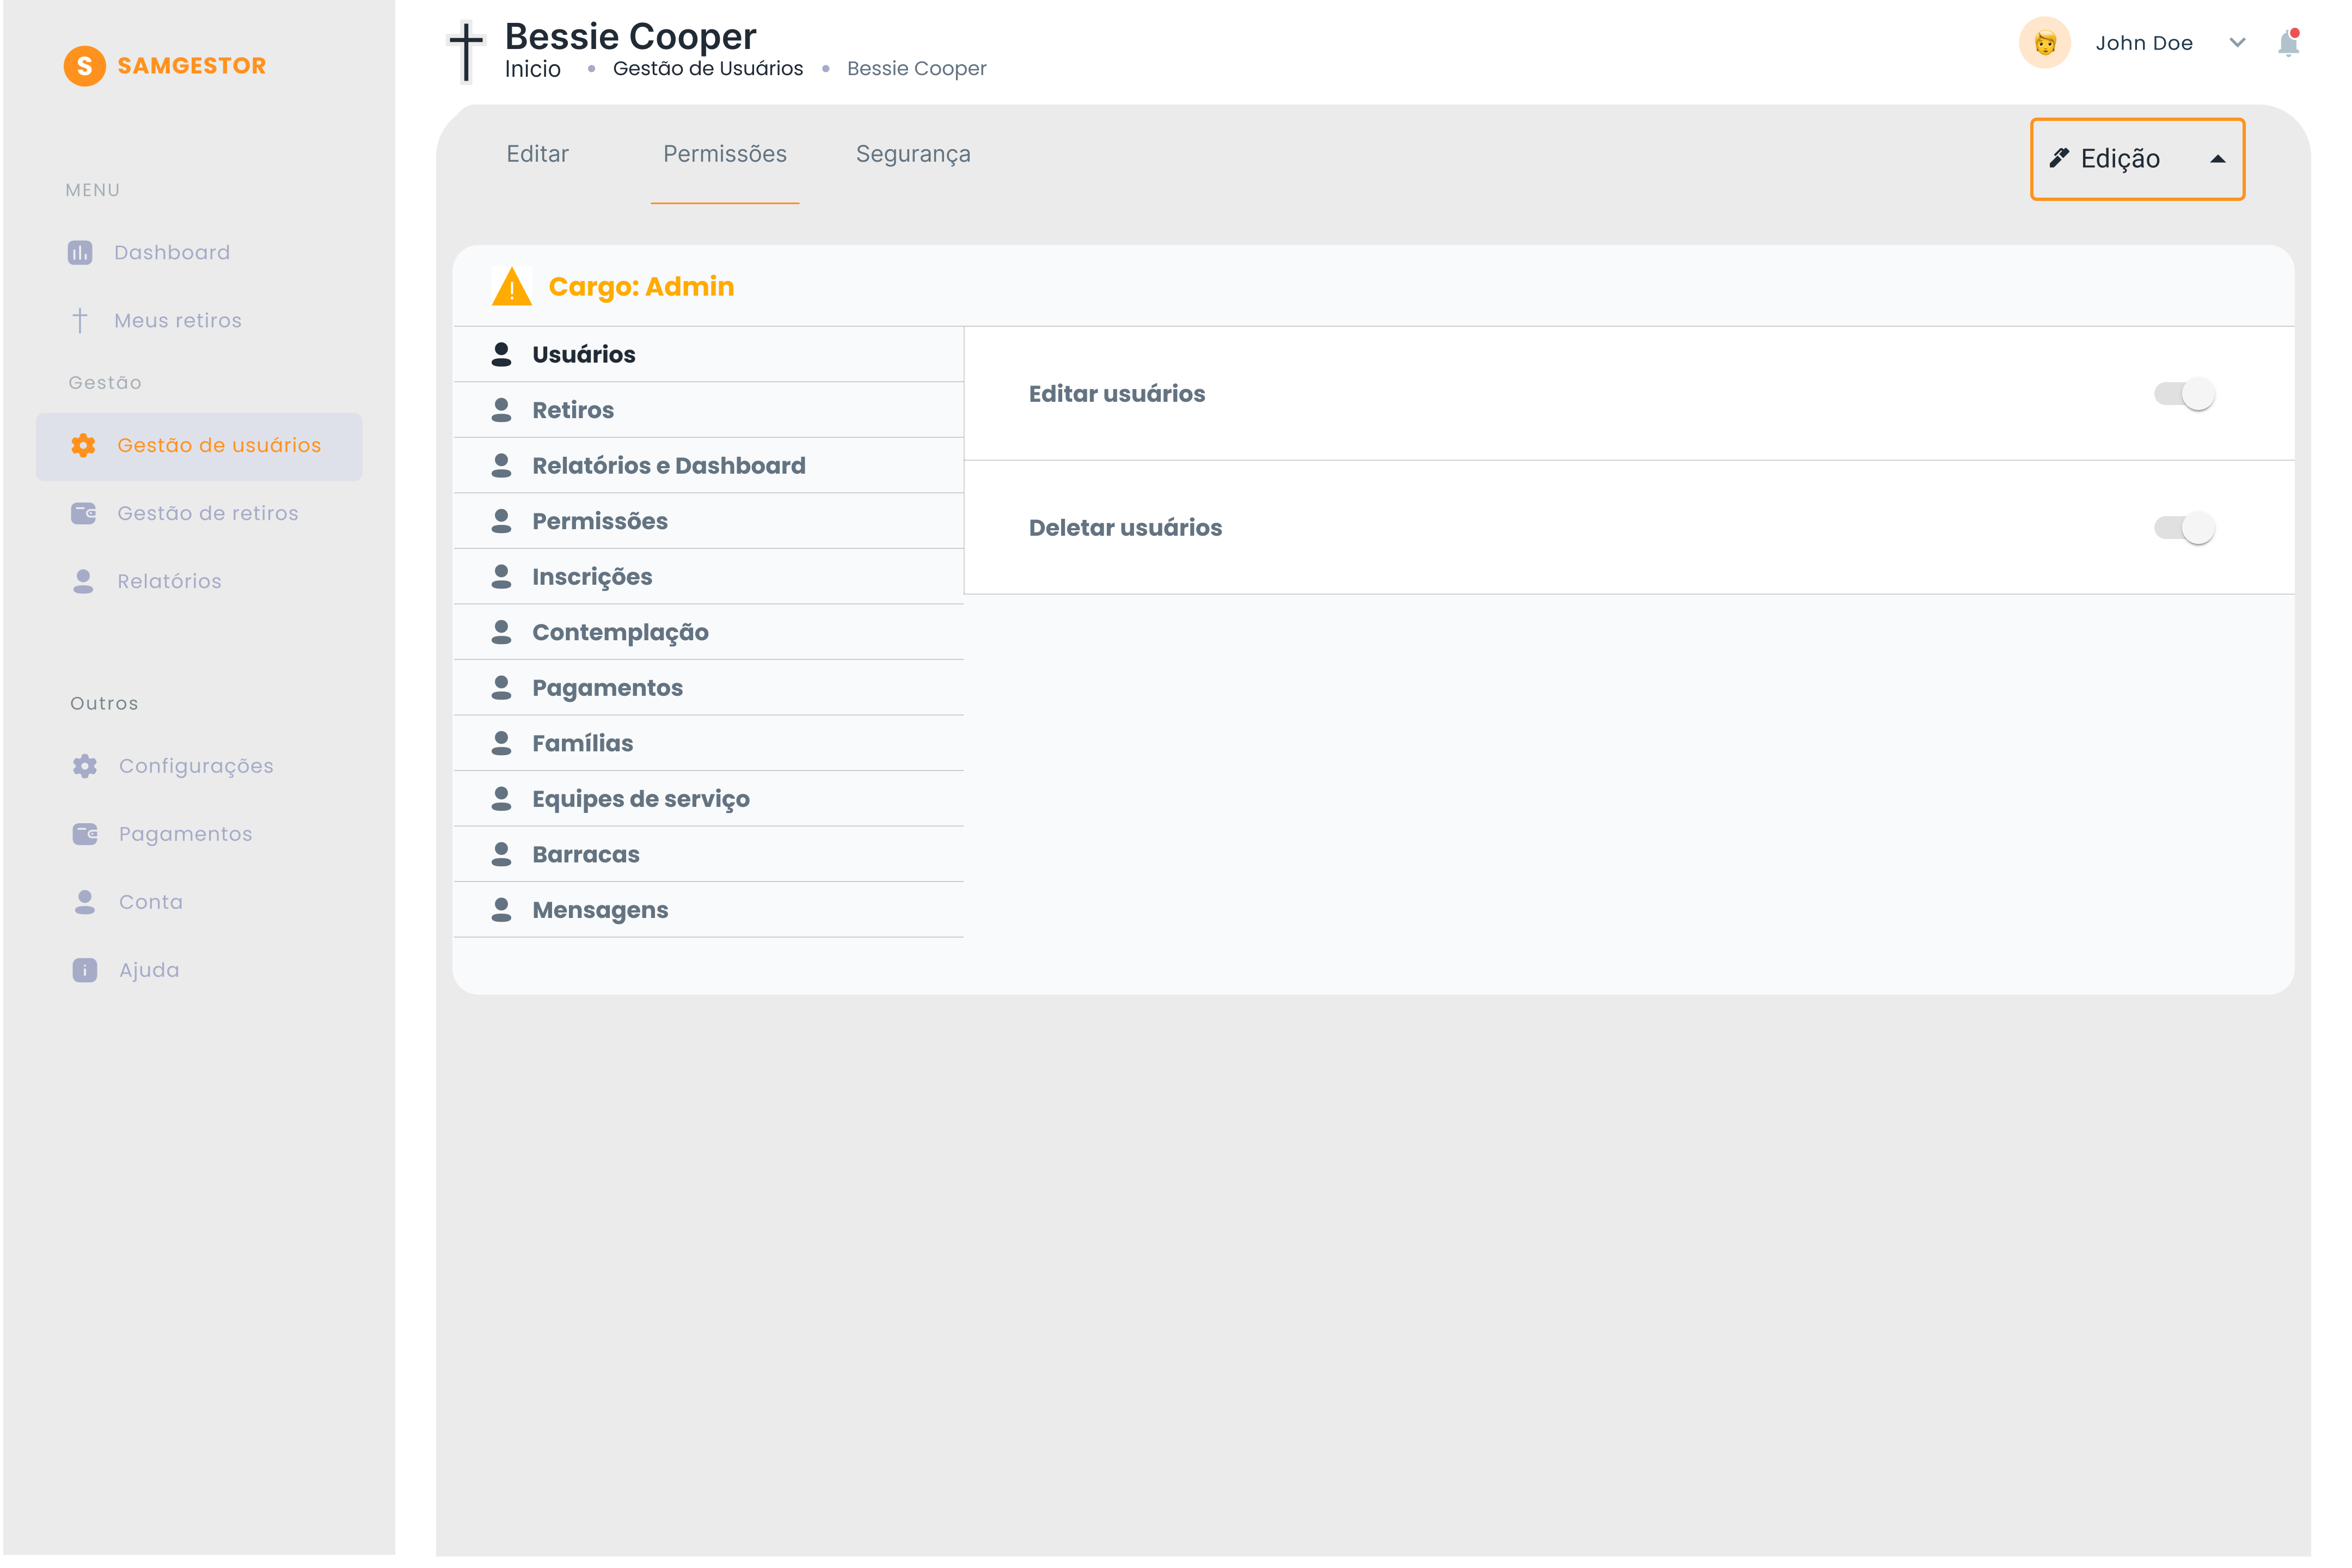
\includegraphics[width=0.8\textwidth]{images/prototipacao/gestao_de_usuarios/Permissões obrigatórias do cargo.png}
\caption{Na tela de permissões, as permissões referentes ao cargo não poderão ser modificadas.}
\end{figure}

\begin{figure}[H]
\centering
\includegraphics[width=0.8\textwidth]{images/prototipacao/gestao_de_usuarios/Credenciais do Usuário.png}
\caption{Tela destinada à redefinição de credenciais de usuários por um administrador do sistema. Esta funcionalidade é utilizada em casos nos quais o usuário perdeu o acesso e não possui e-mail confirmado para recuperação. Por questões de segurança e privacidade, o administrador não visualiza as credenciais atuais do usuário — apenas define valores provisórios. Ao realizar o primeiro acesso com as novas credenciais, o próprio usuário será solicitado a redefini-las. O acesso a esta funcionalidade requer autenticação adicional do administrador mediante digitação da sua senha.}
\end{figure}

\begin{figure}[H]
\centering
\includegraphics[width=0.8\textwidth]{images/prototipacao/gestao_retiros_geral/Gestão de Retiros Geral.png}
\caption{Tela inicial do módulo de gestão de retiros. Apresenta funcionalidades para visualização, edição, criação e exclusão de registros de retiros, permitindo ao usuário administrador gerenciar eficientemente os eventos cadastrados no sistema.}
\end{figure}

\begin{figure}[H]
\centering
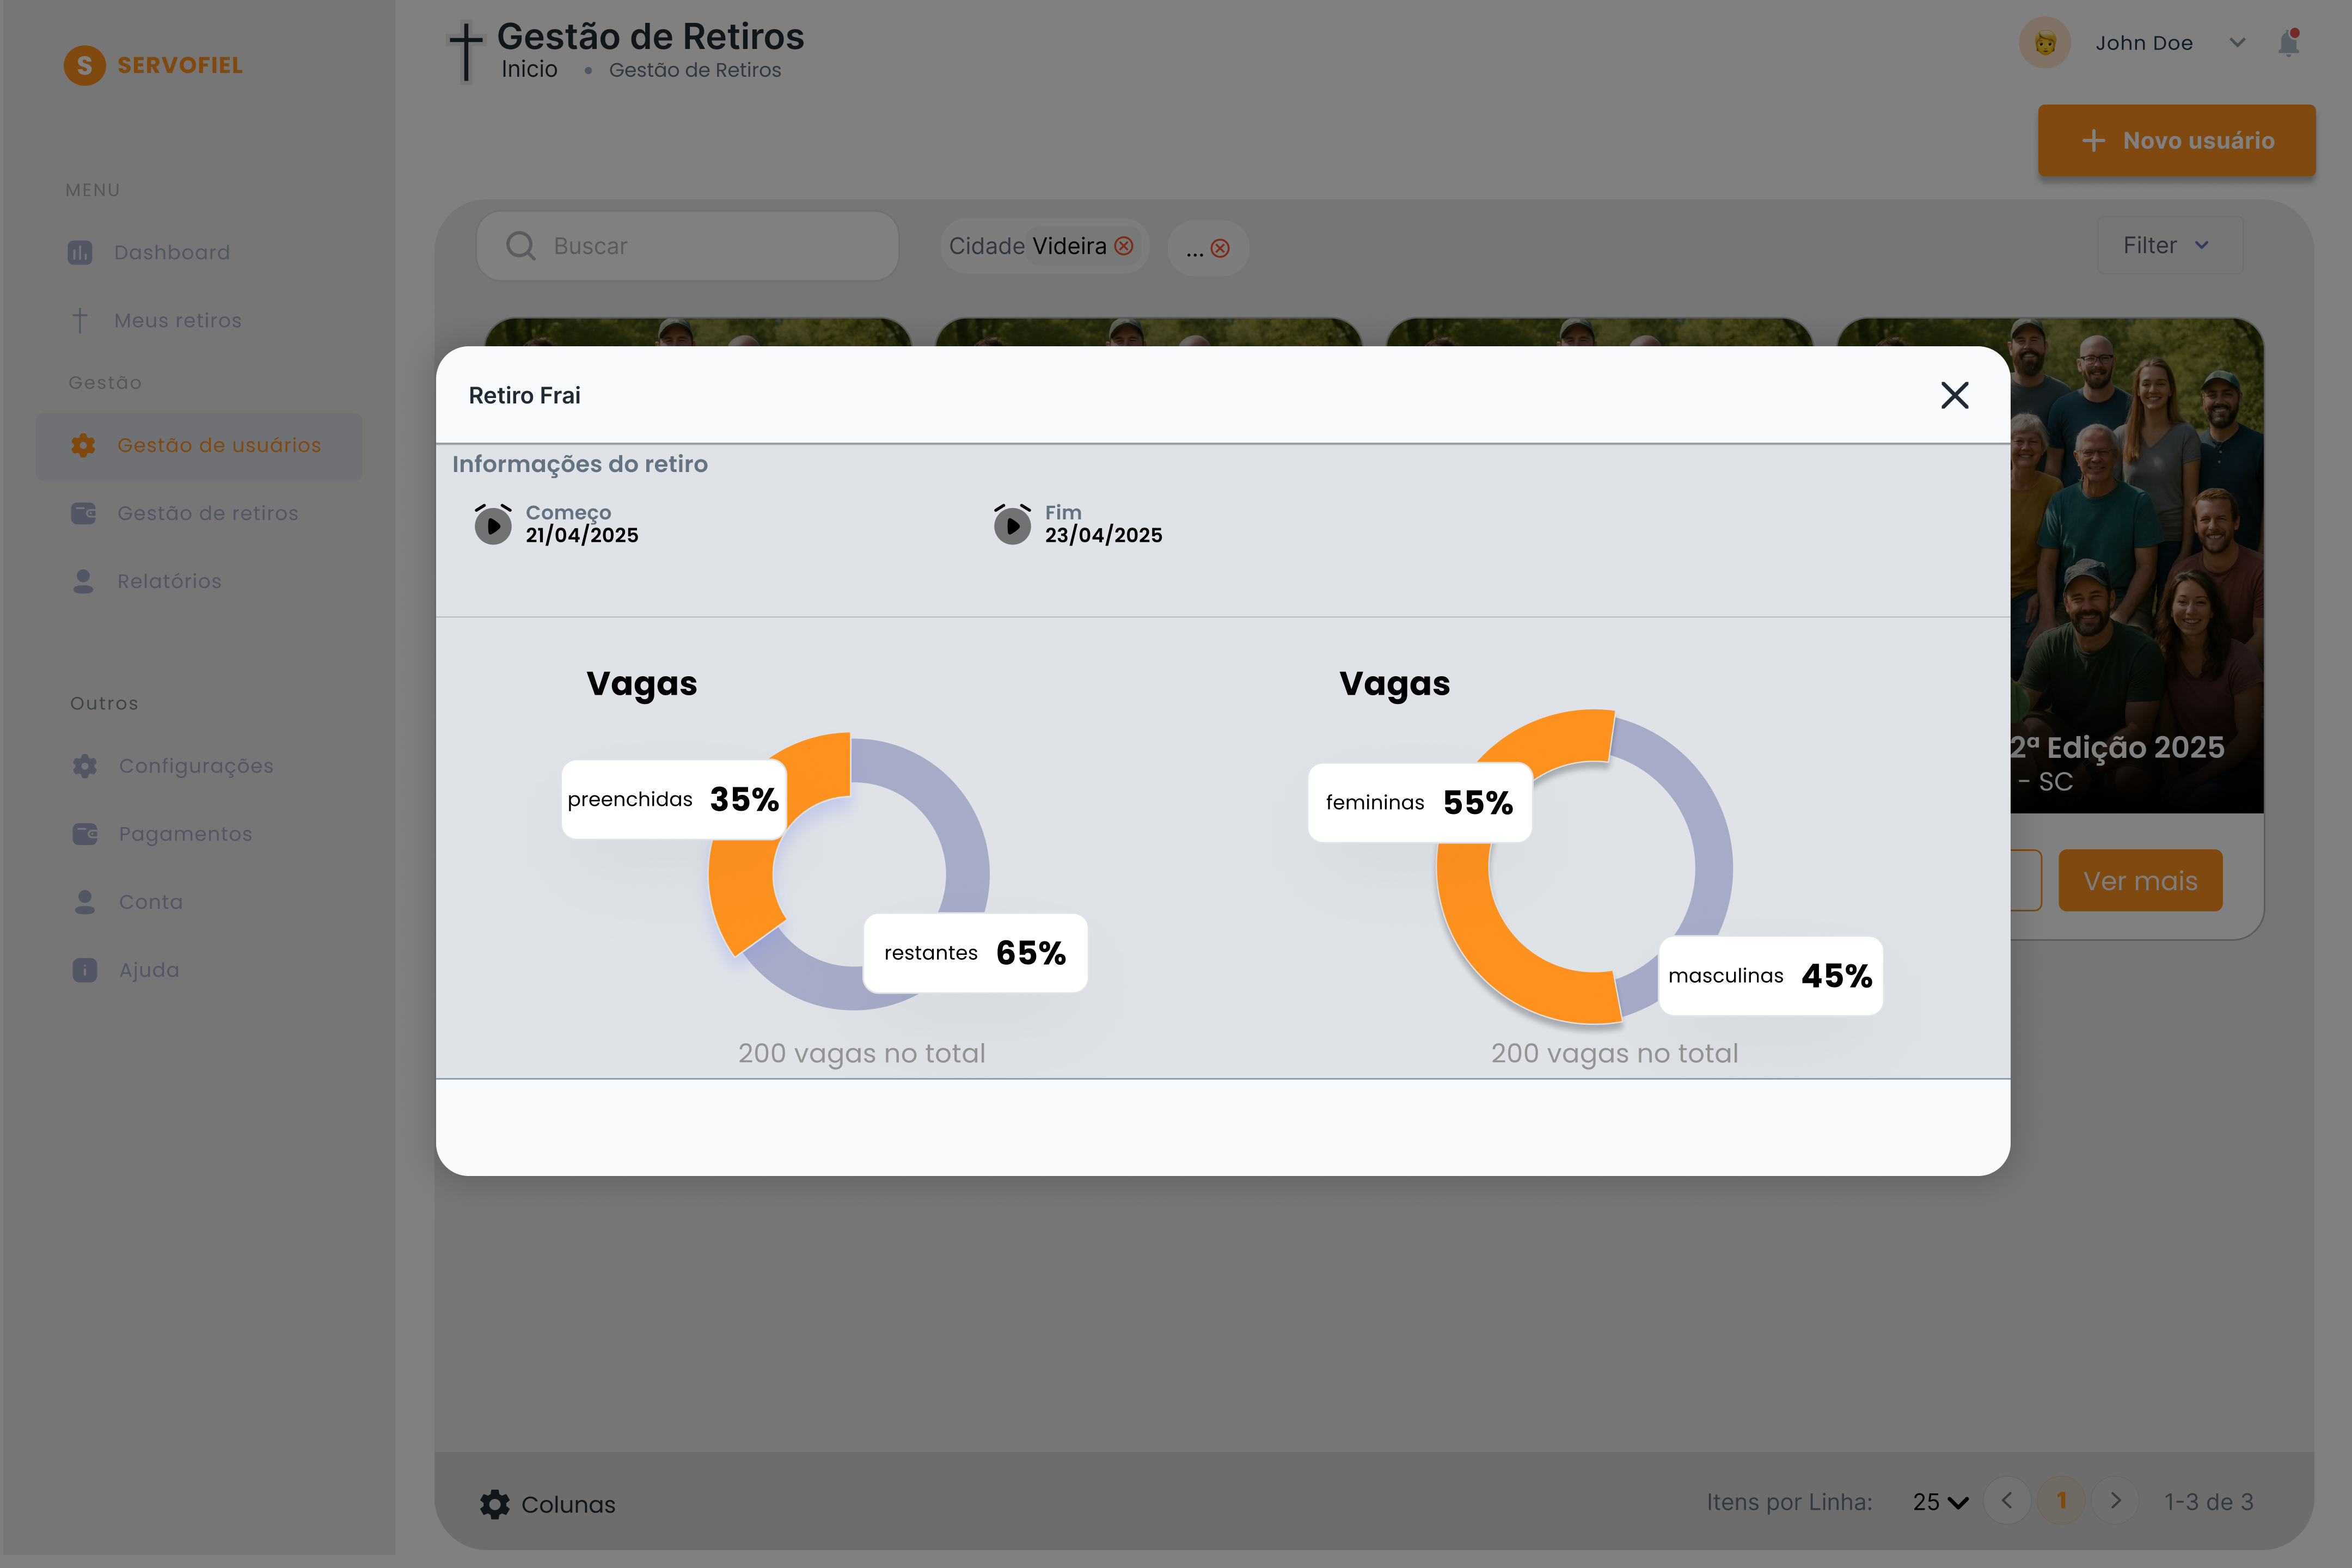
\includegraphics[width=0.8\textwidth]{images/prototipacao/gestao_retiros_geral/Ver Mais Retiro.png}
\caption{Ao clicar no botão "Ver mais", uma modal com informações do retiro é aberta.}
\end{figure}

\begin{figure}[H]
\centering
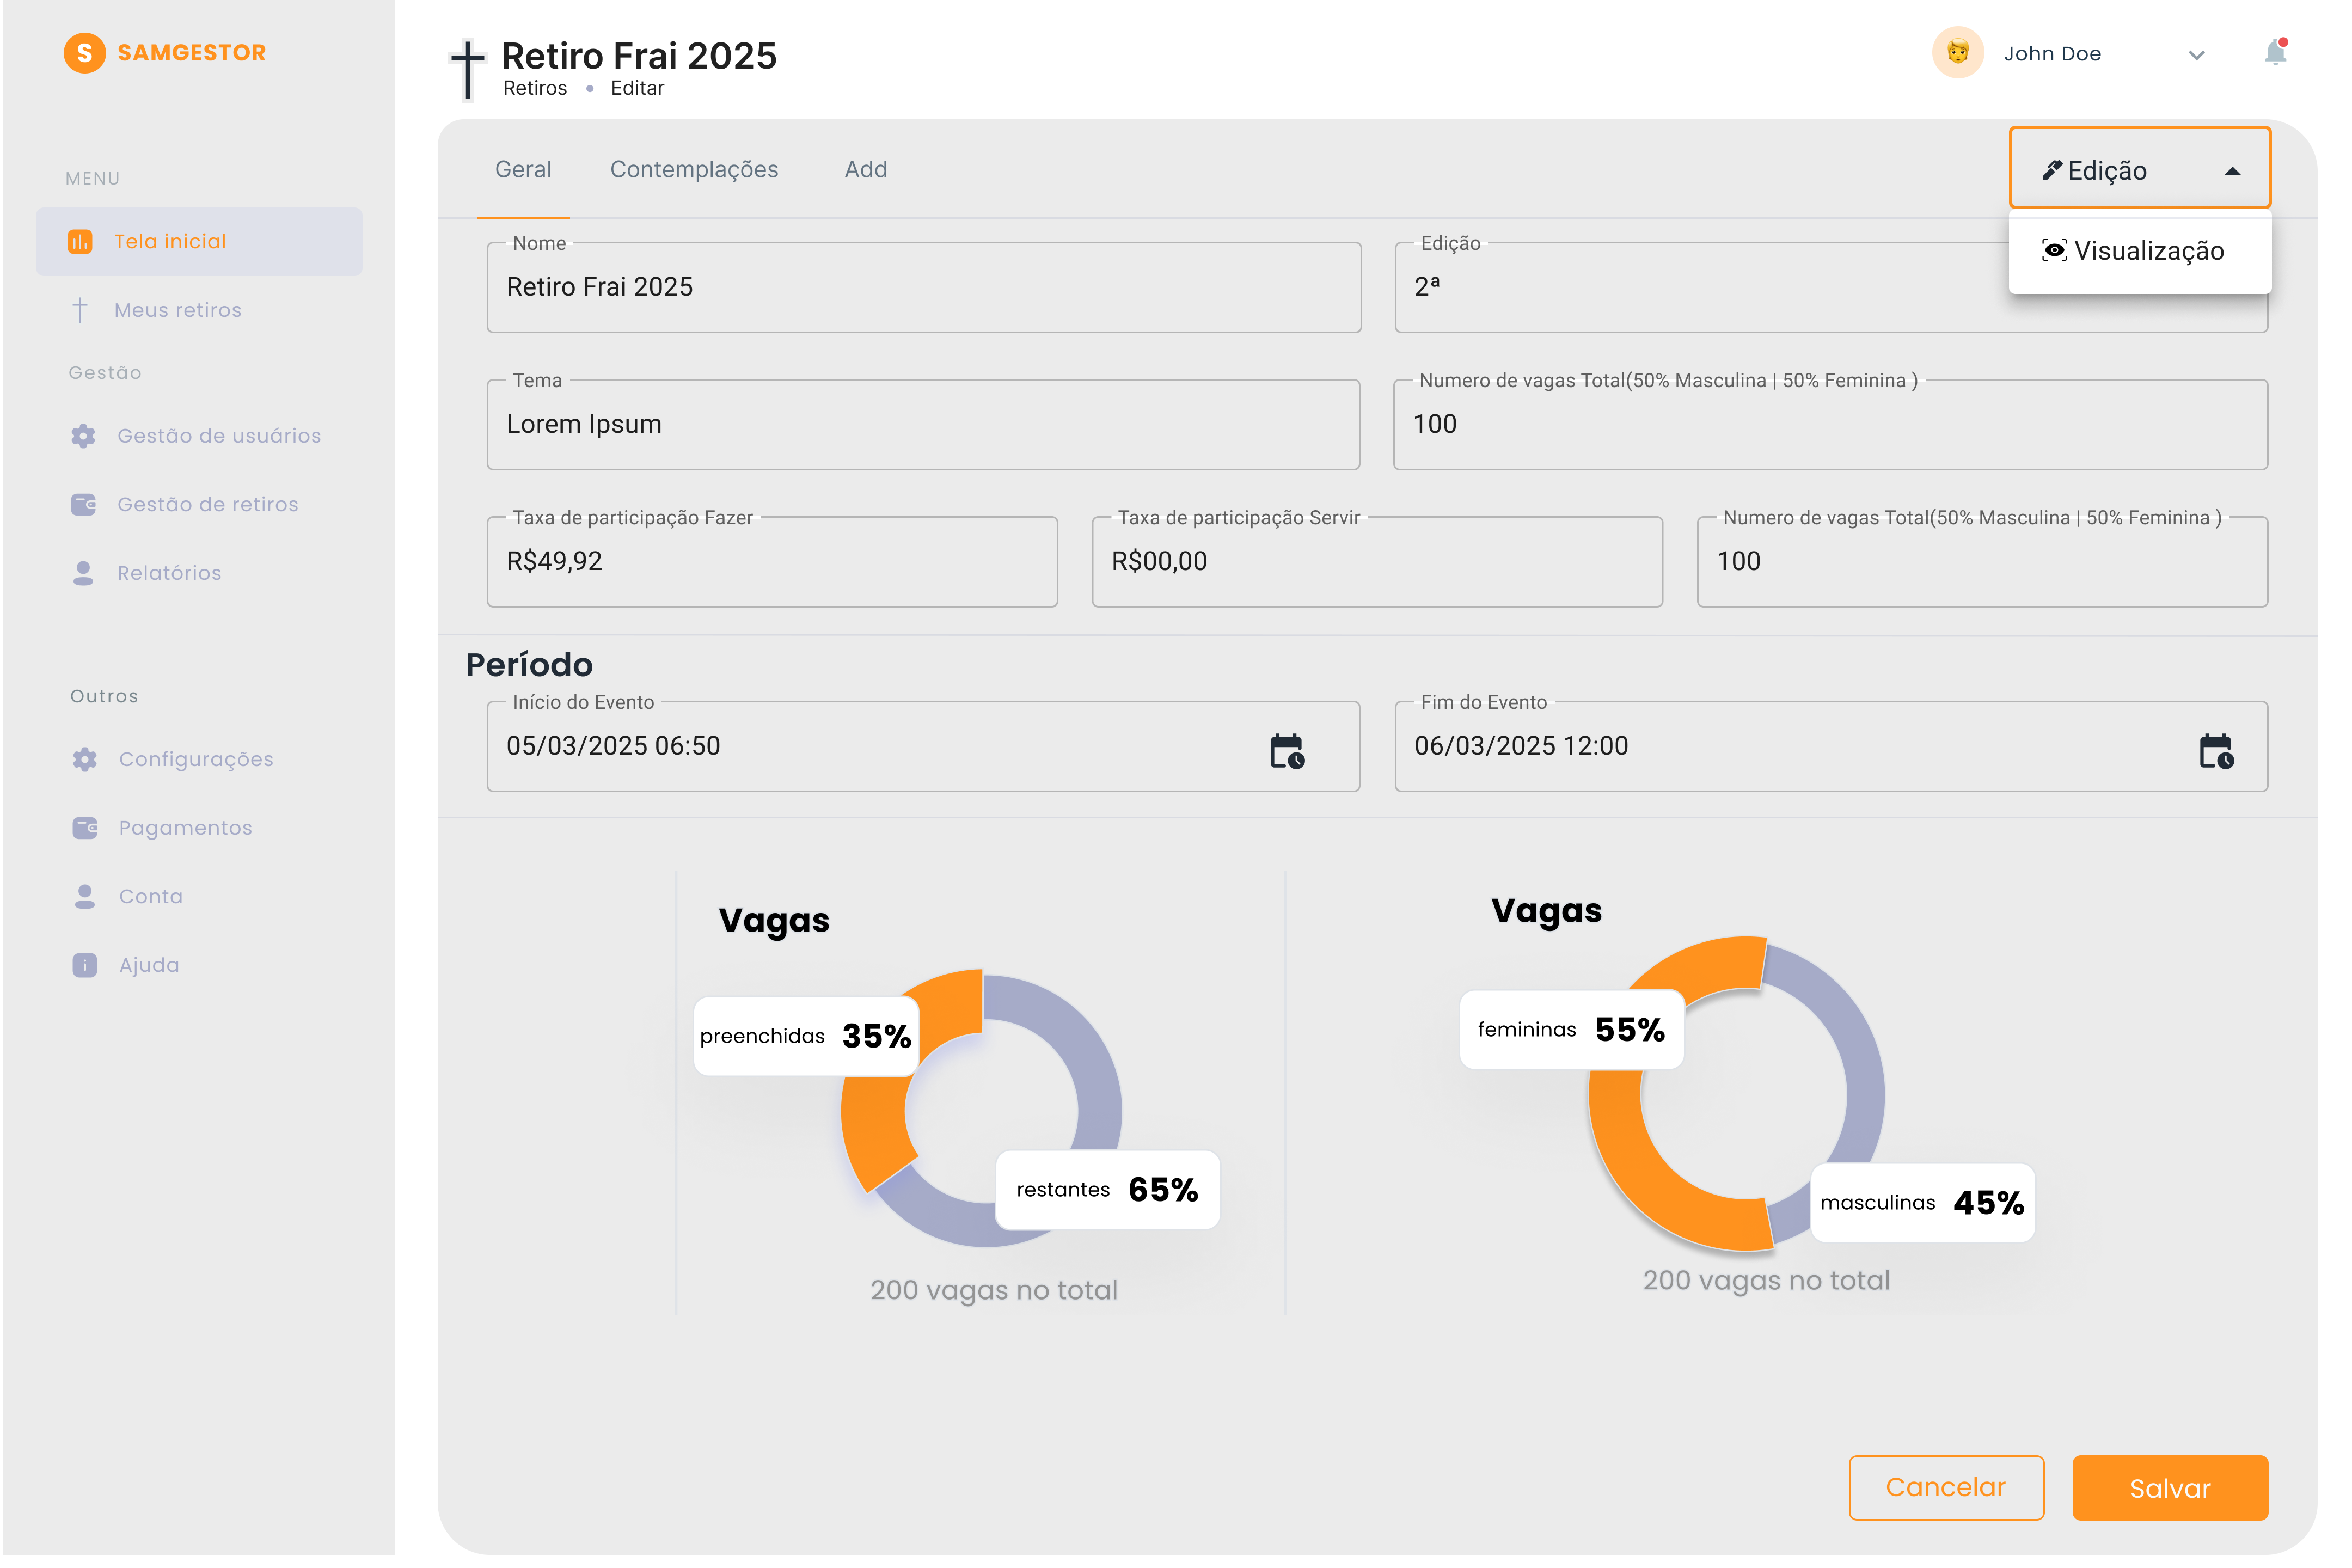
\includegraphics[width=0.8\textwidth]{images/prototipacao/gestao_retiros_geral/Geral.png}
\caption{Formulário de criação ou edição do retiro.}
\end{figure}

\begin{figure}[H]
\centering
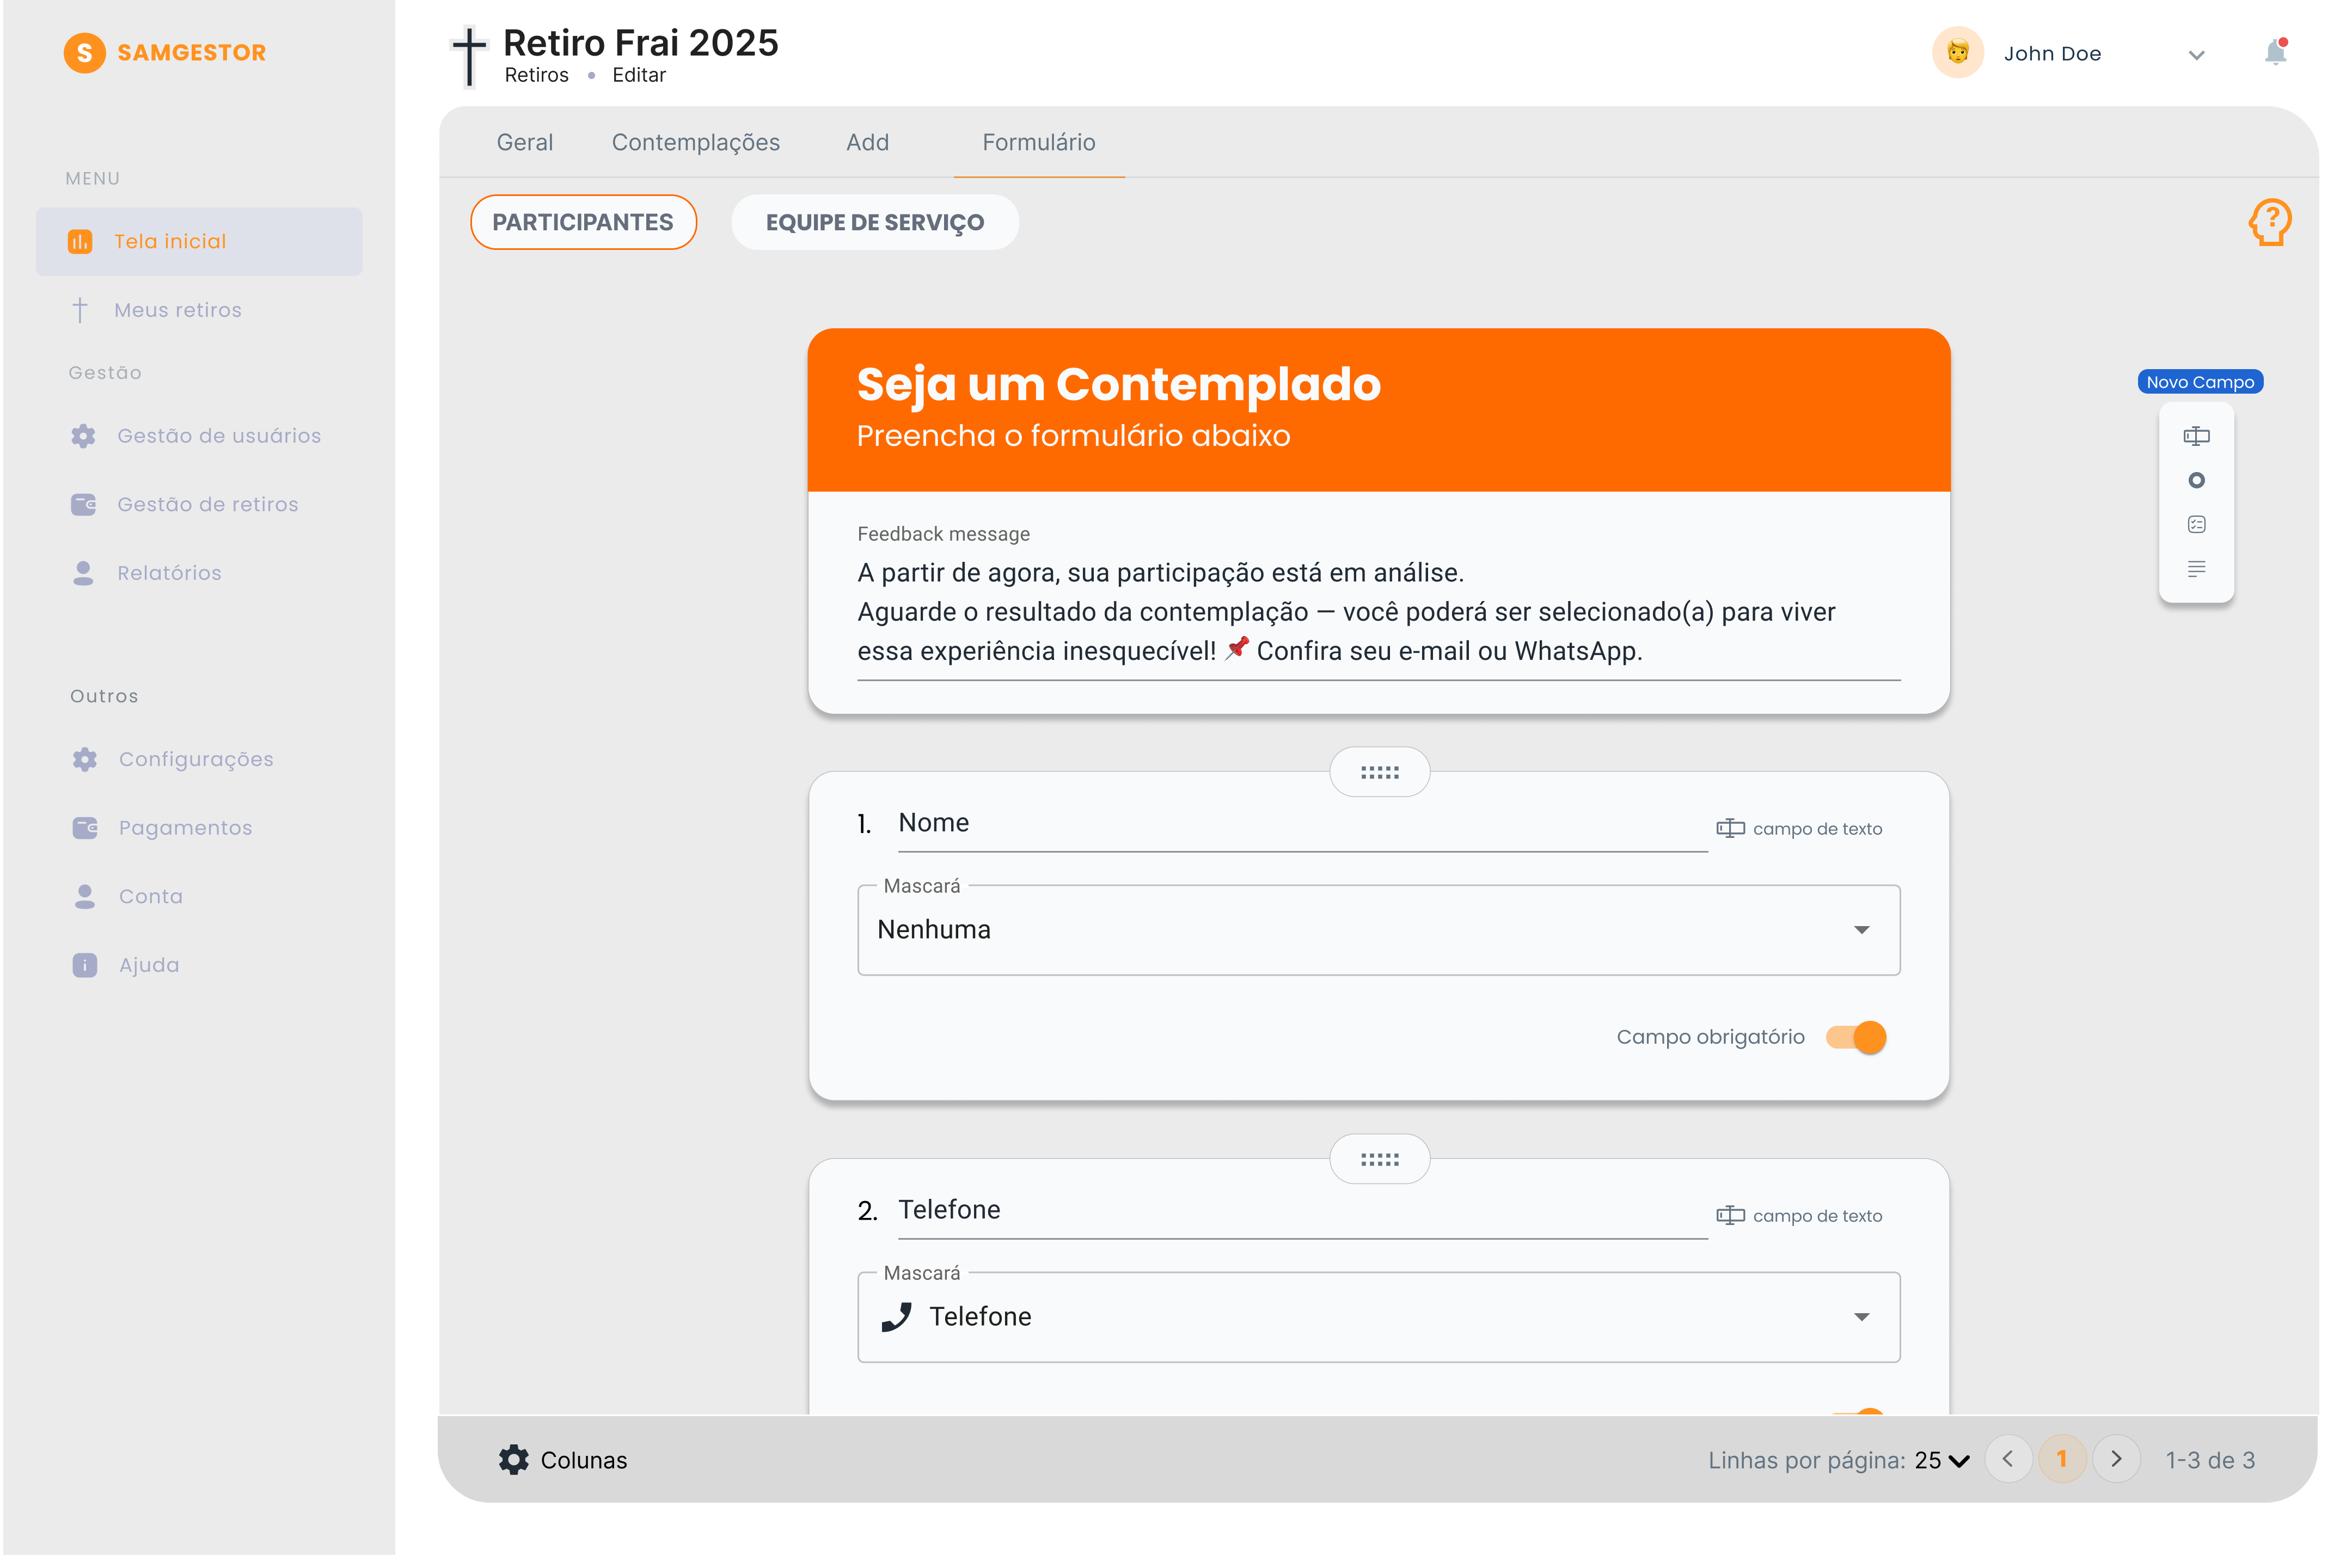
\includegraphics[width=0.8\textwidth]{images/prototipacao/gestao_retiros_geral/Formulario.png}
\caption{Ferramenta para criação de formulários, onde o gestor irá decidir o título, descrição, ordem e nome dos campos.}
\end{figure}

\begin{figure}[H]
\centering
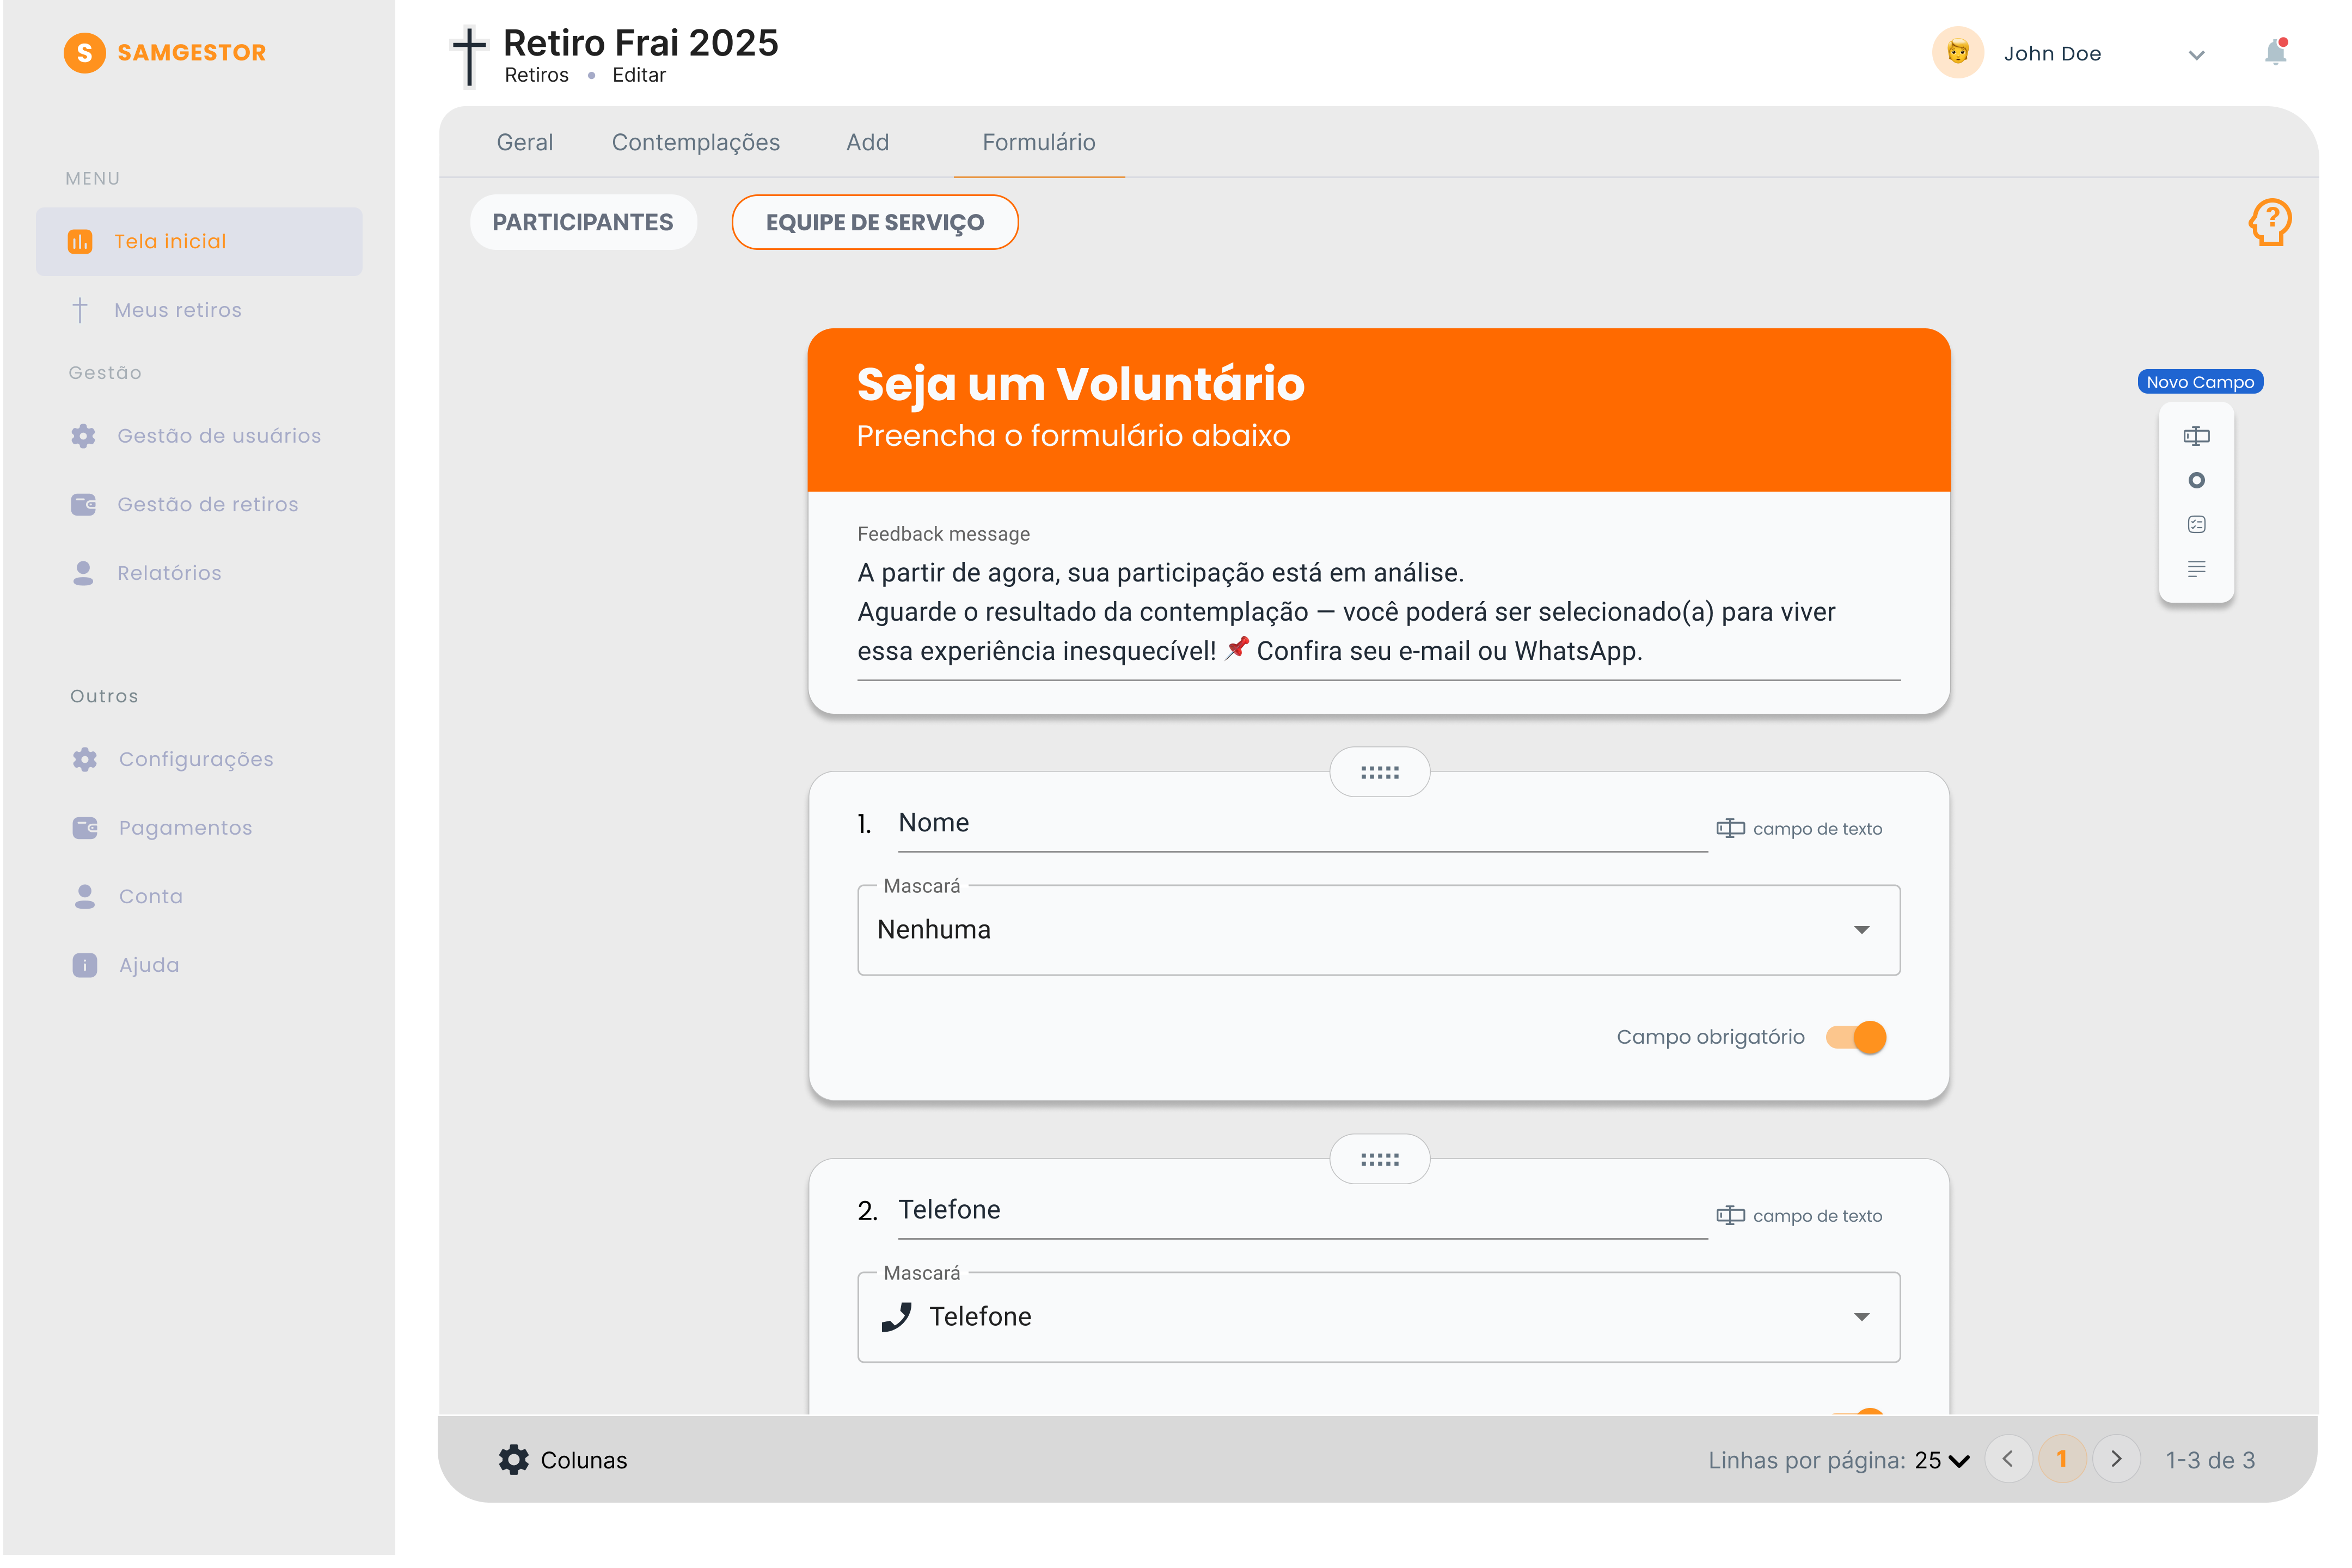
\includegraphics[width=0.8\textwidth]{images/prototipacao/gestao_retiros_geral/FormularioEquipeDeServico.png}
\caption{Aba de criação do formulário para a equipe de serviço.}
\end{figure}

\begin{figure}[H]
\centering
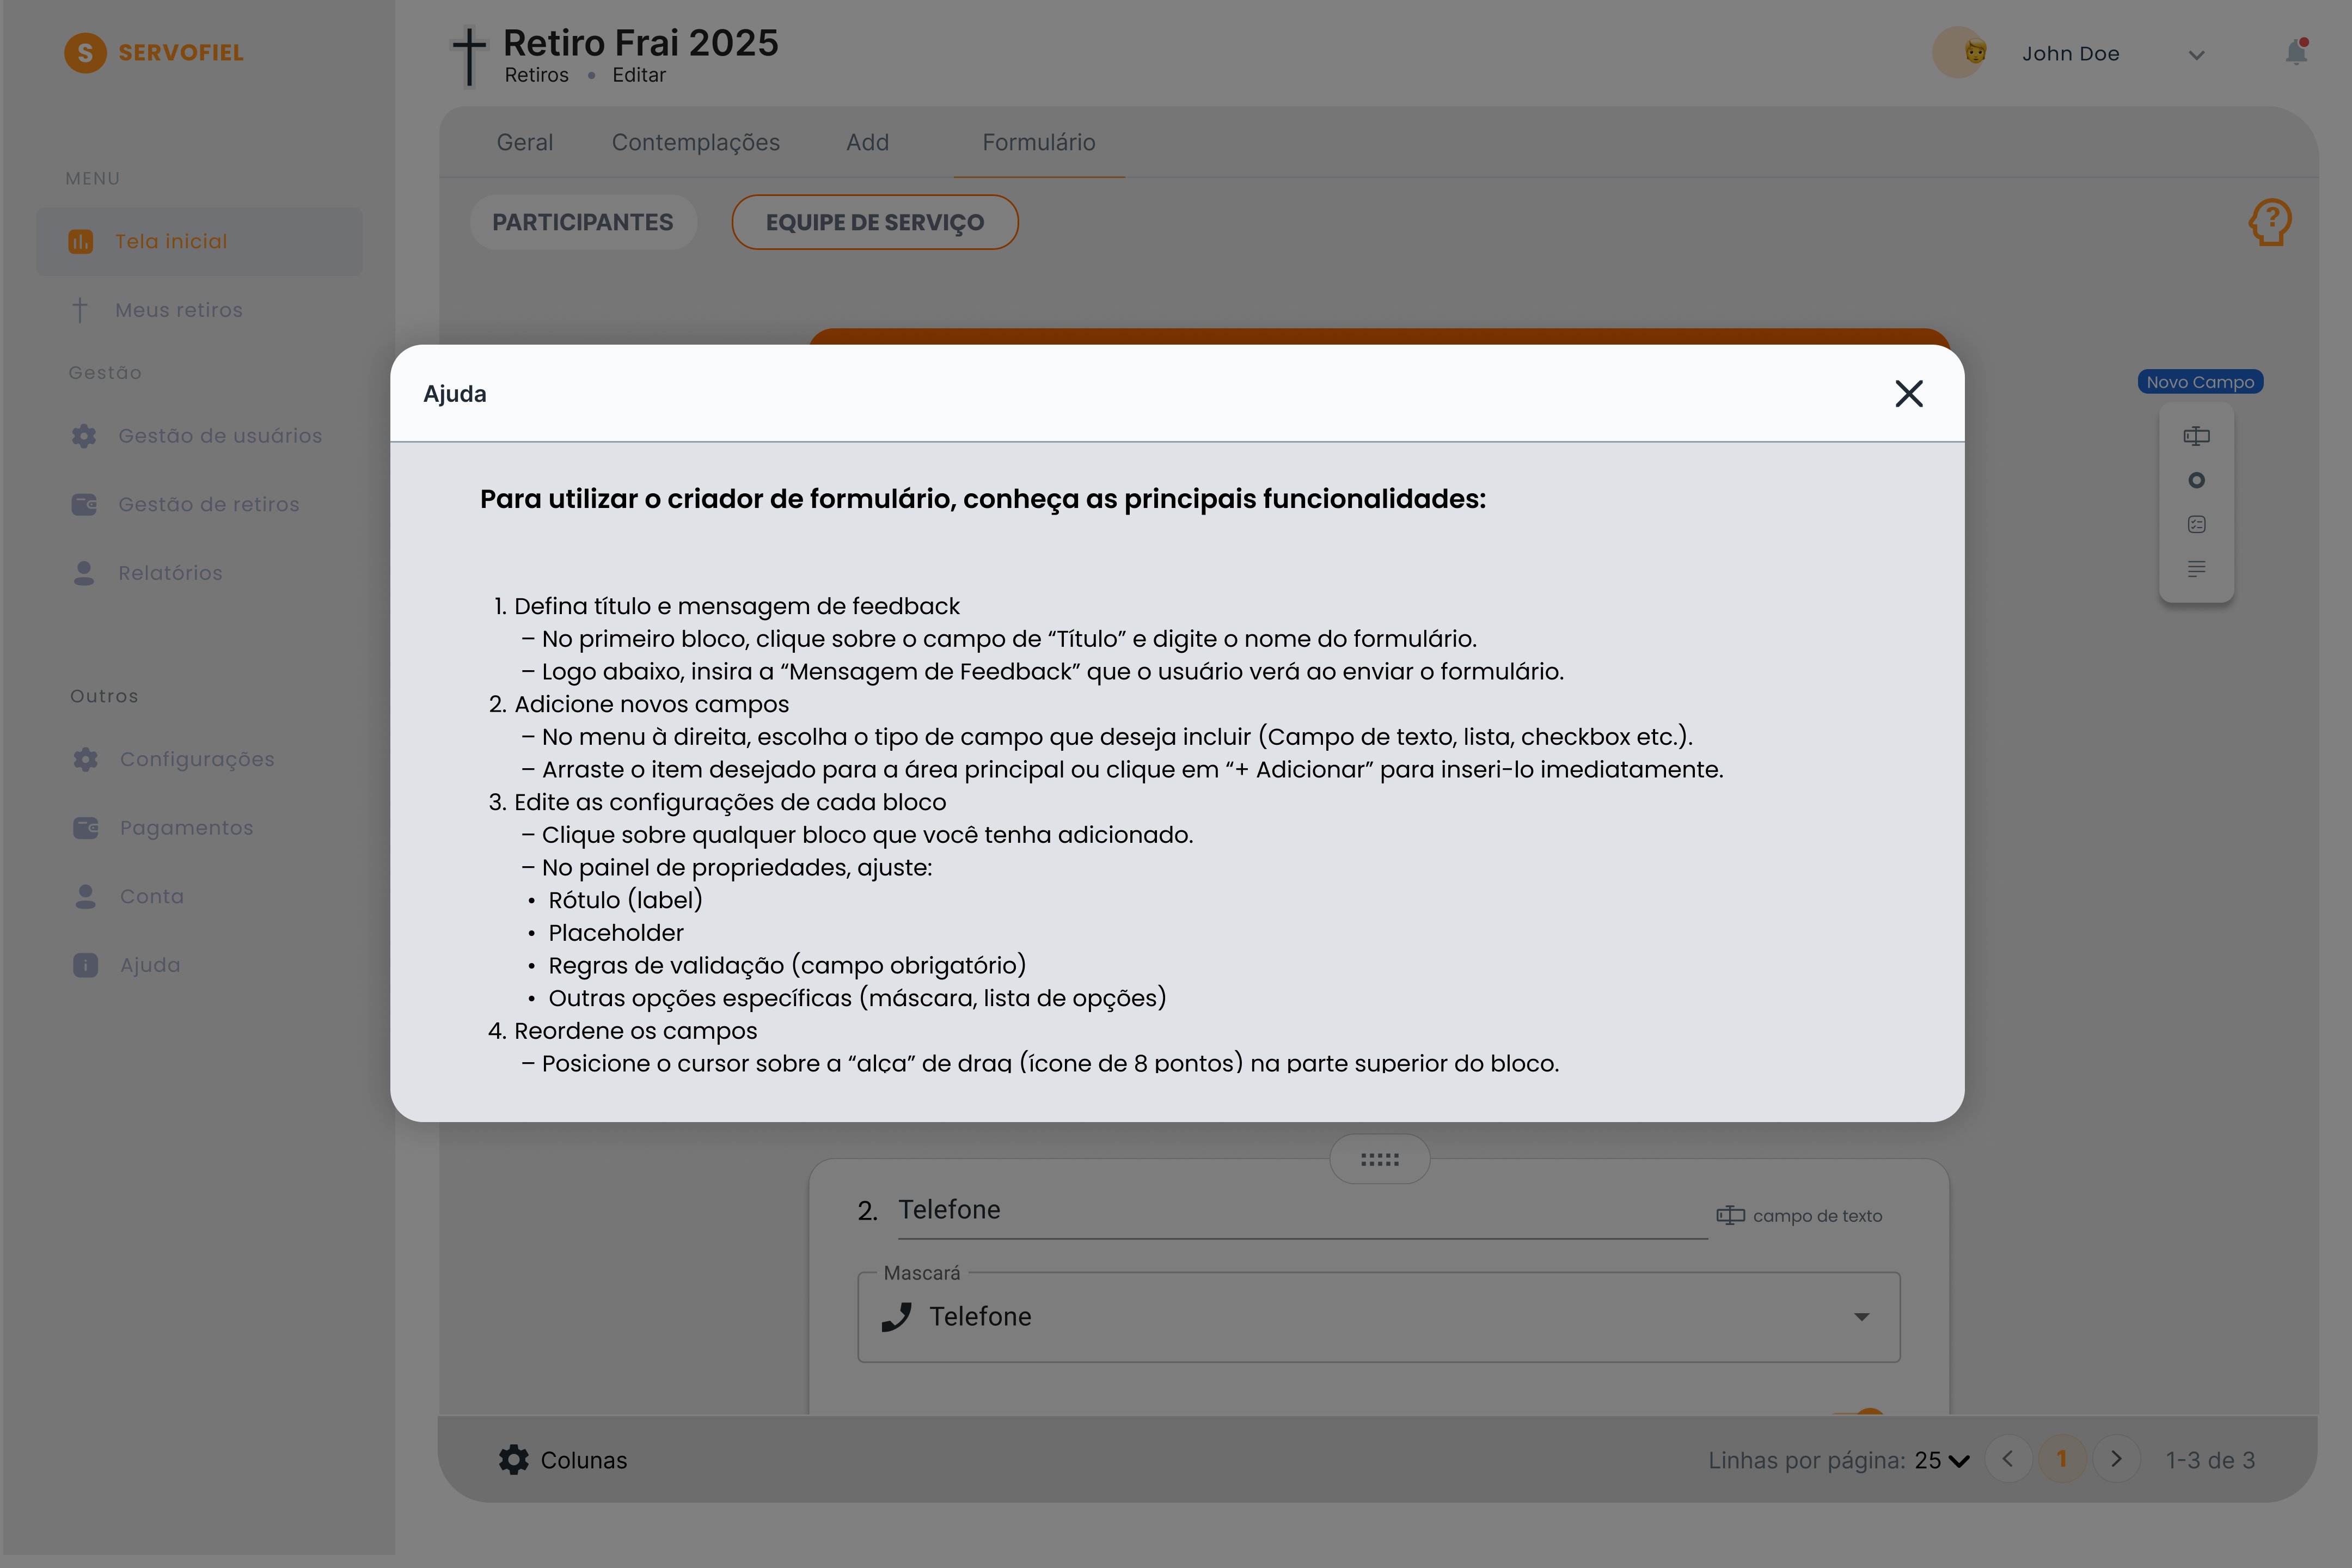
\includegraphics[width=0.8\textwidth]{images/prototipacao/gestao_retiros_geral/Ajuda.png}
\caption{Modal de ajuda com informações de como utilizar a ferramenta construtura de formulários.}
\end{figure}

\begin{figure}[H]
\centering
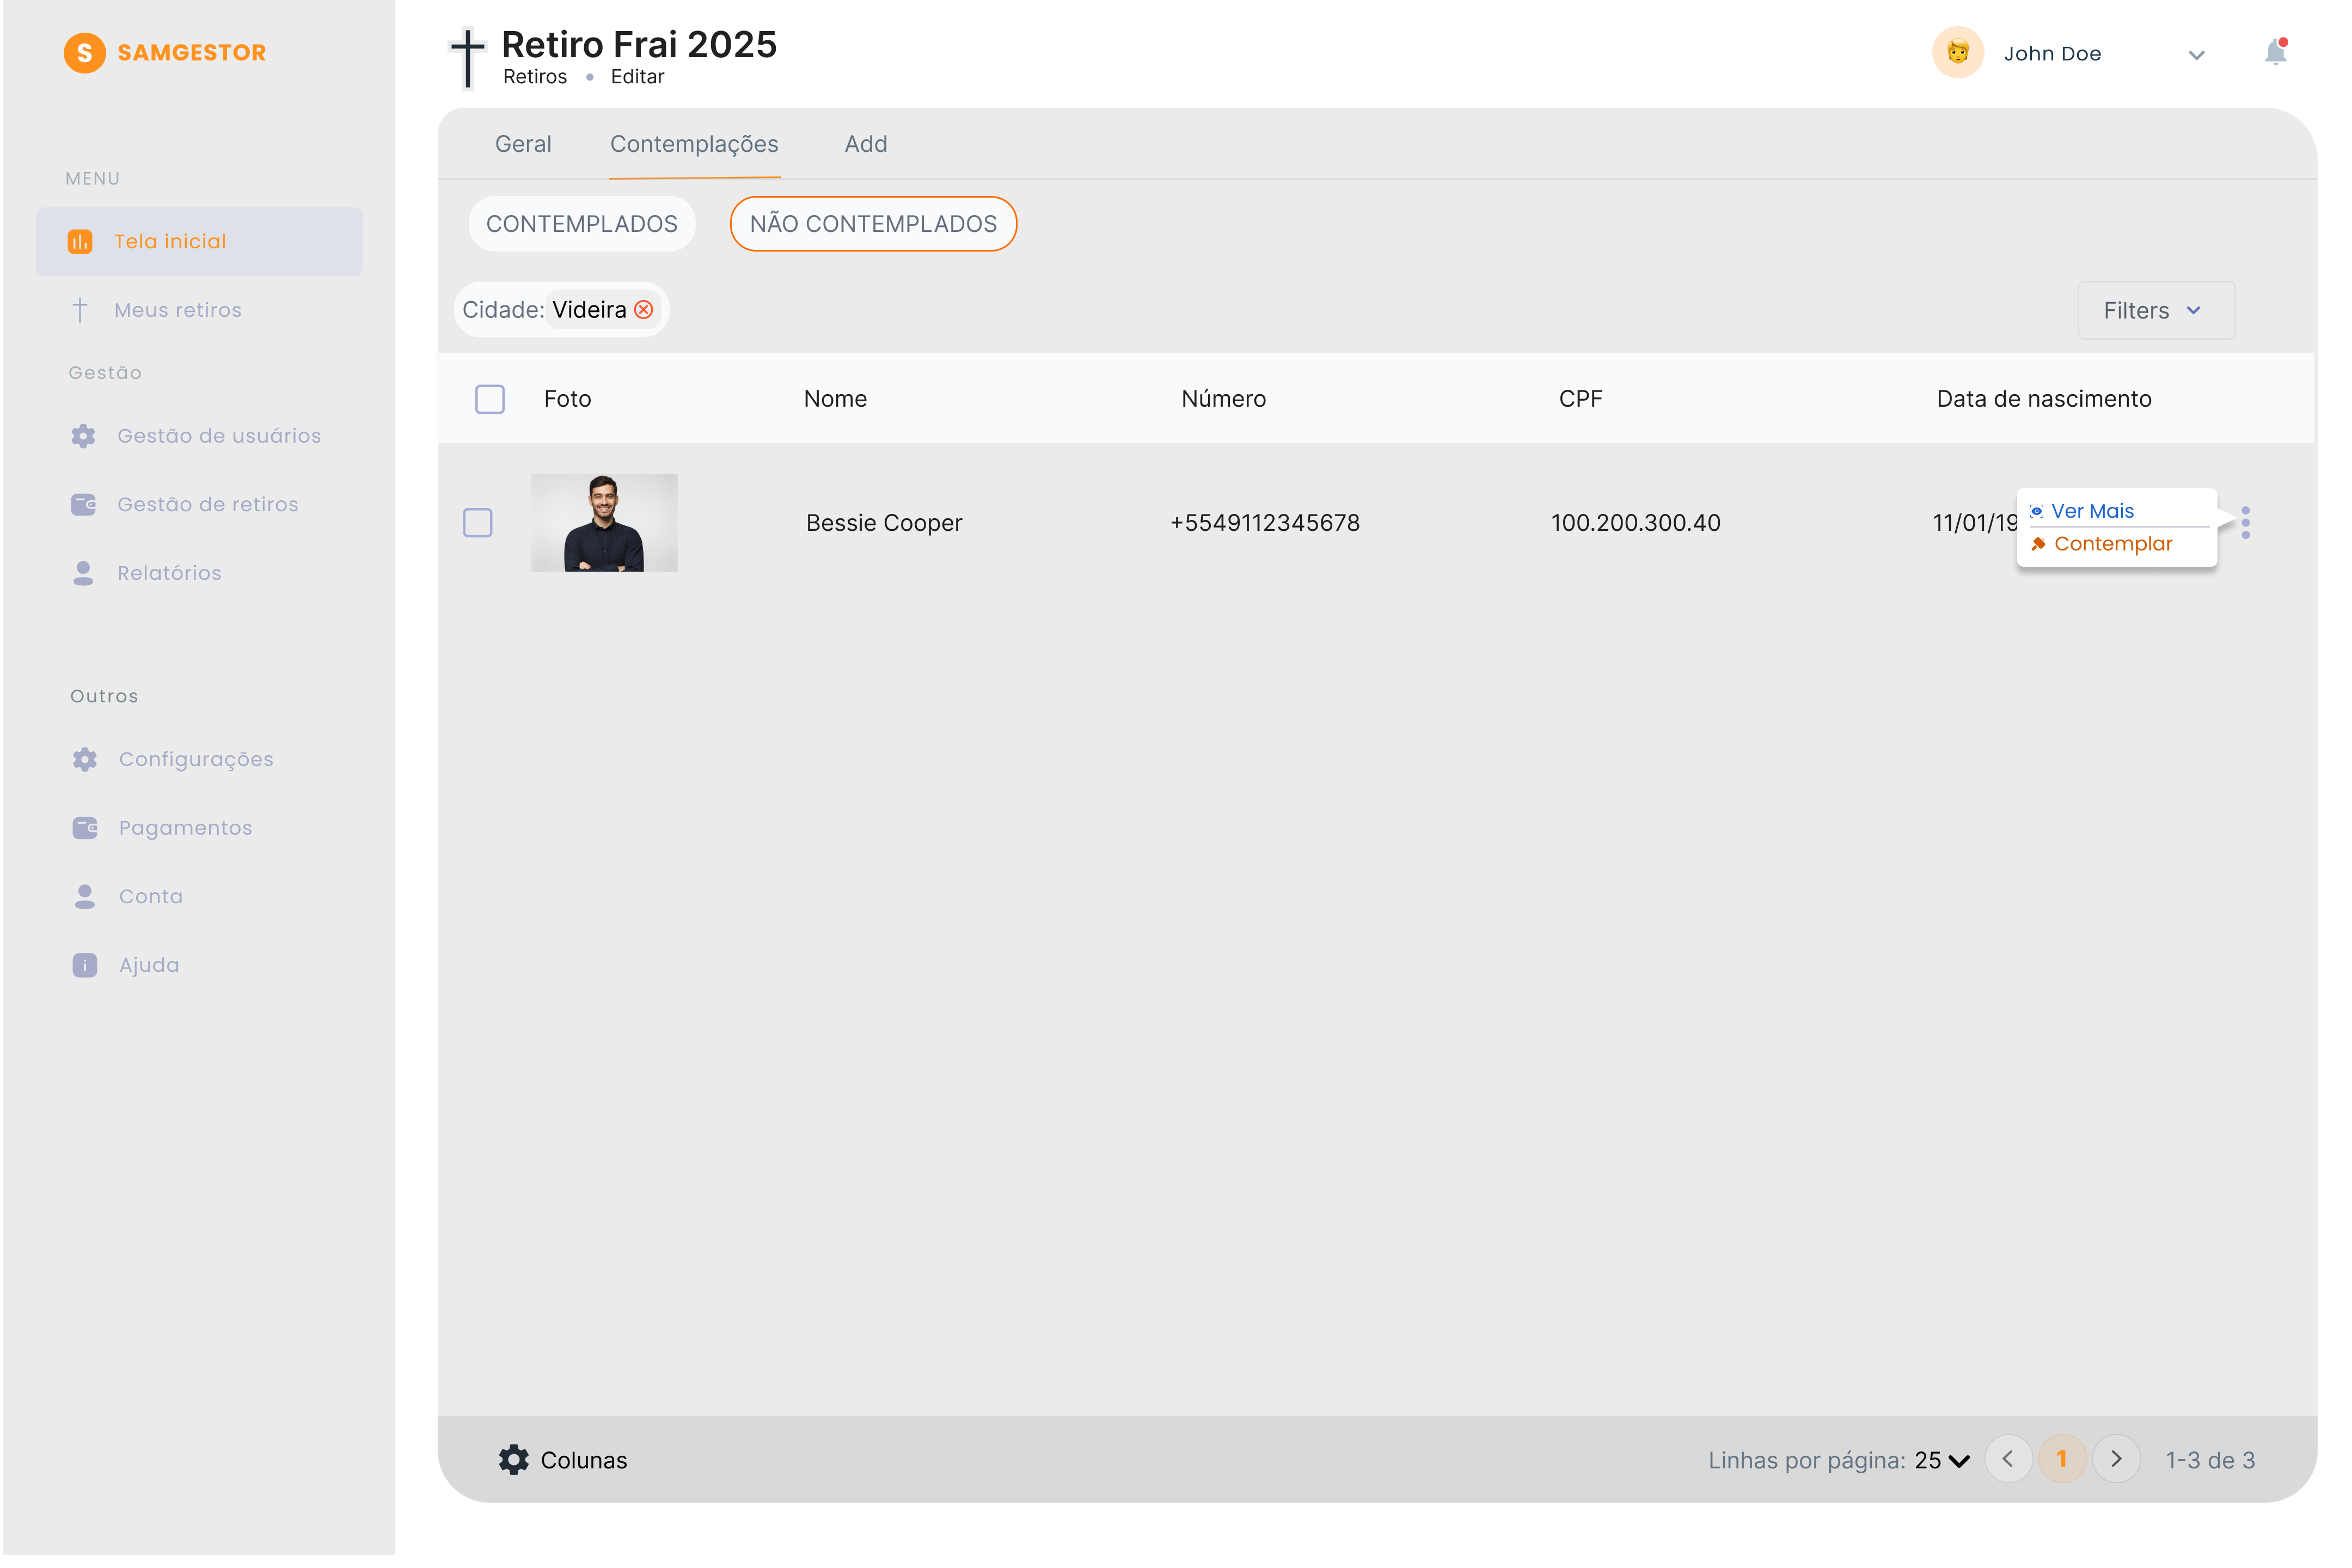
\includegraphics[width=0.8\textwidth]{images/prototipacao/gestao_retiros_geral/NaoContemplados.png}
\caption{Tabela de participantes não contemplados. Permite ao gestor visualizar os inscritos ainda não selecionados para o retiro. Através do menu de contexto (acesso via botão direito do mouse), é possível contemplar o participante ou acessar detalhes adicionais por meio da opção "Ver mais informações".}
\end{figure}

\begin{figure}[H]
\centering
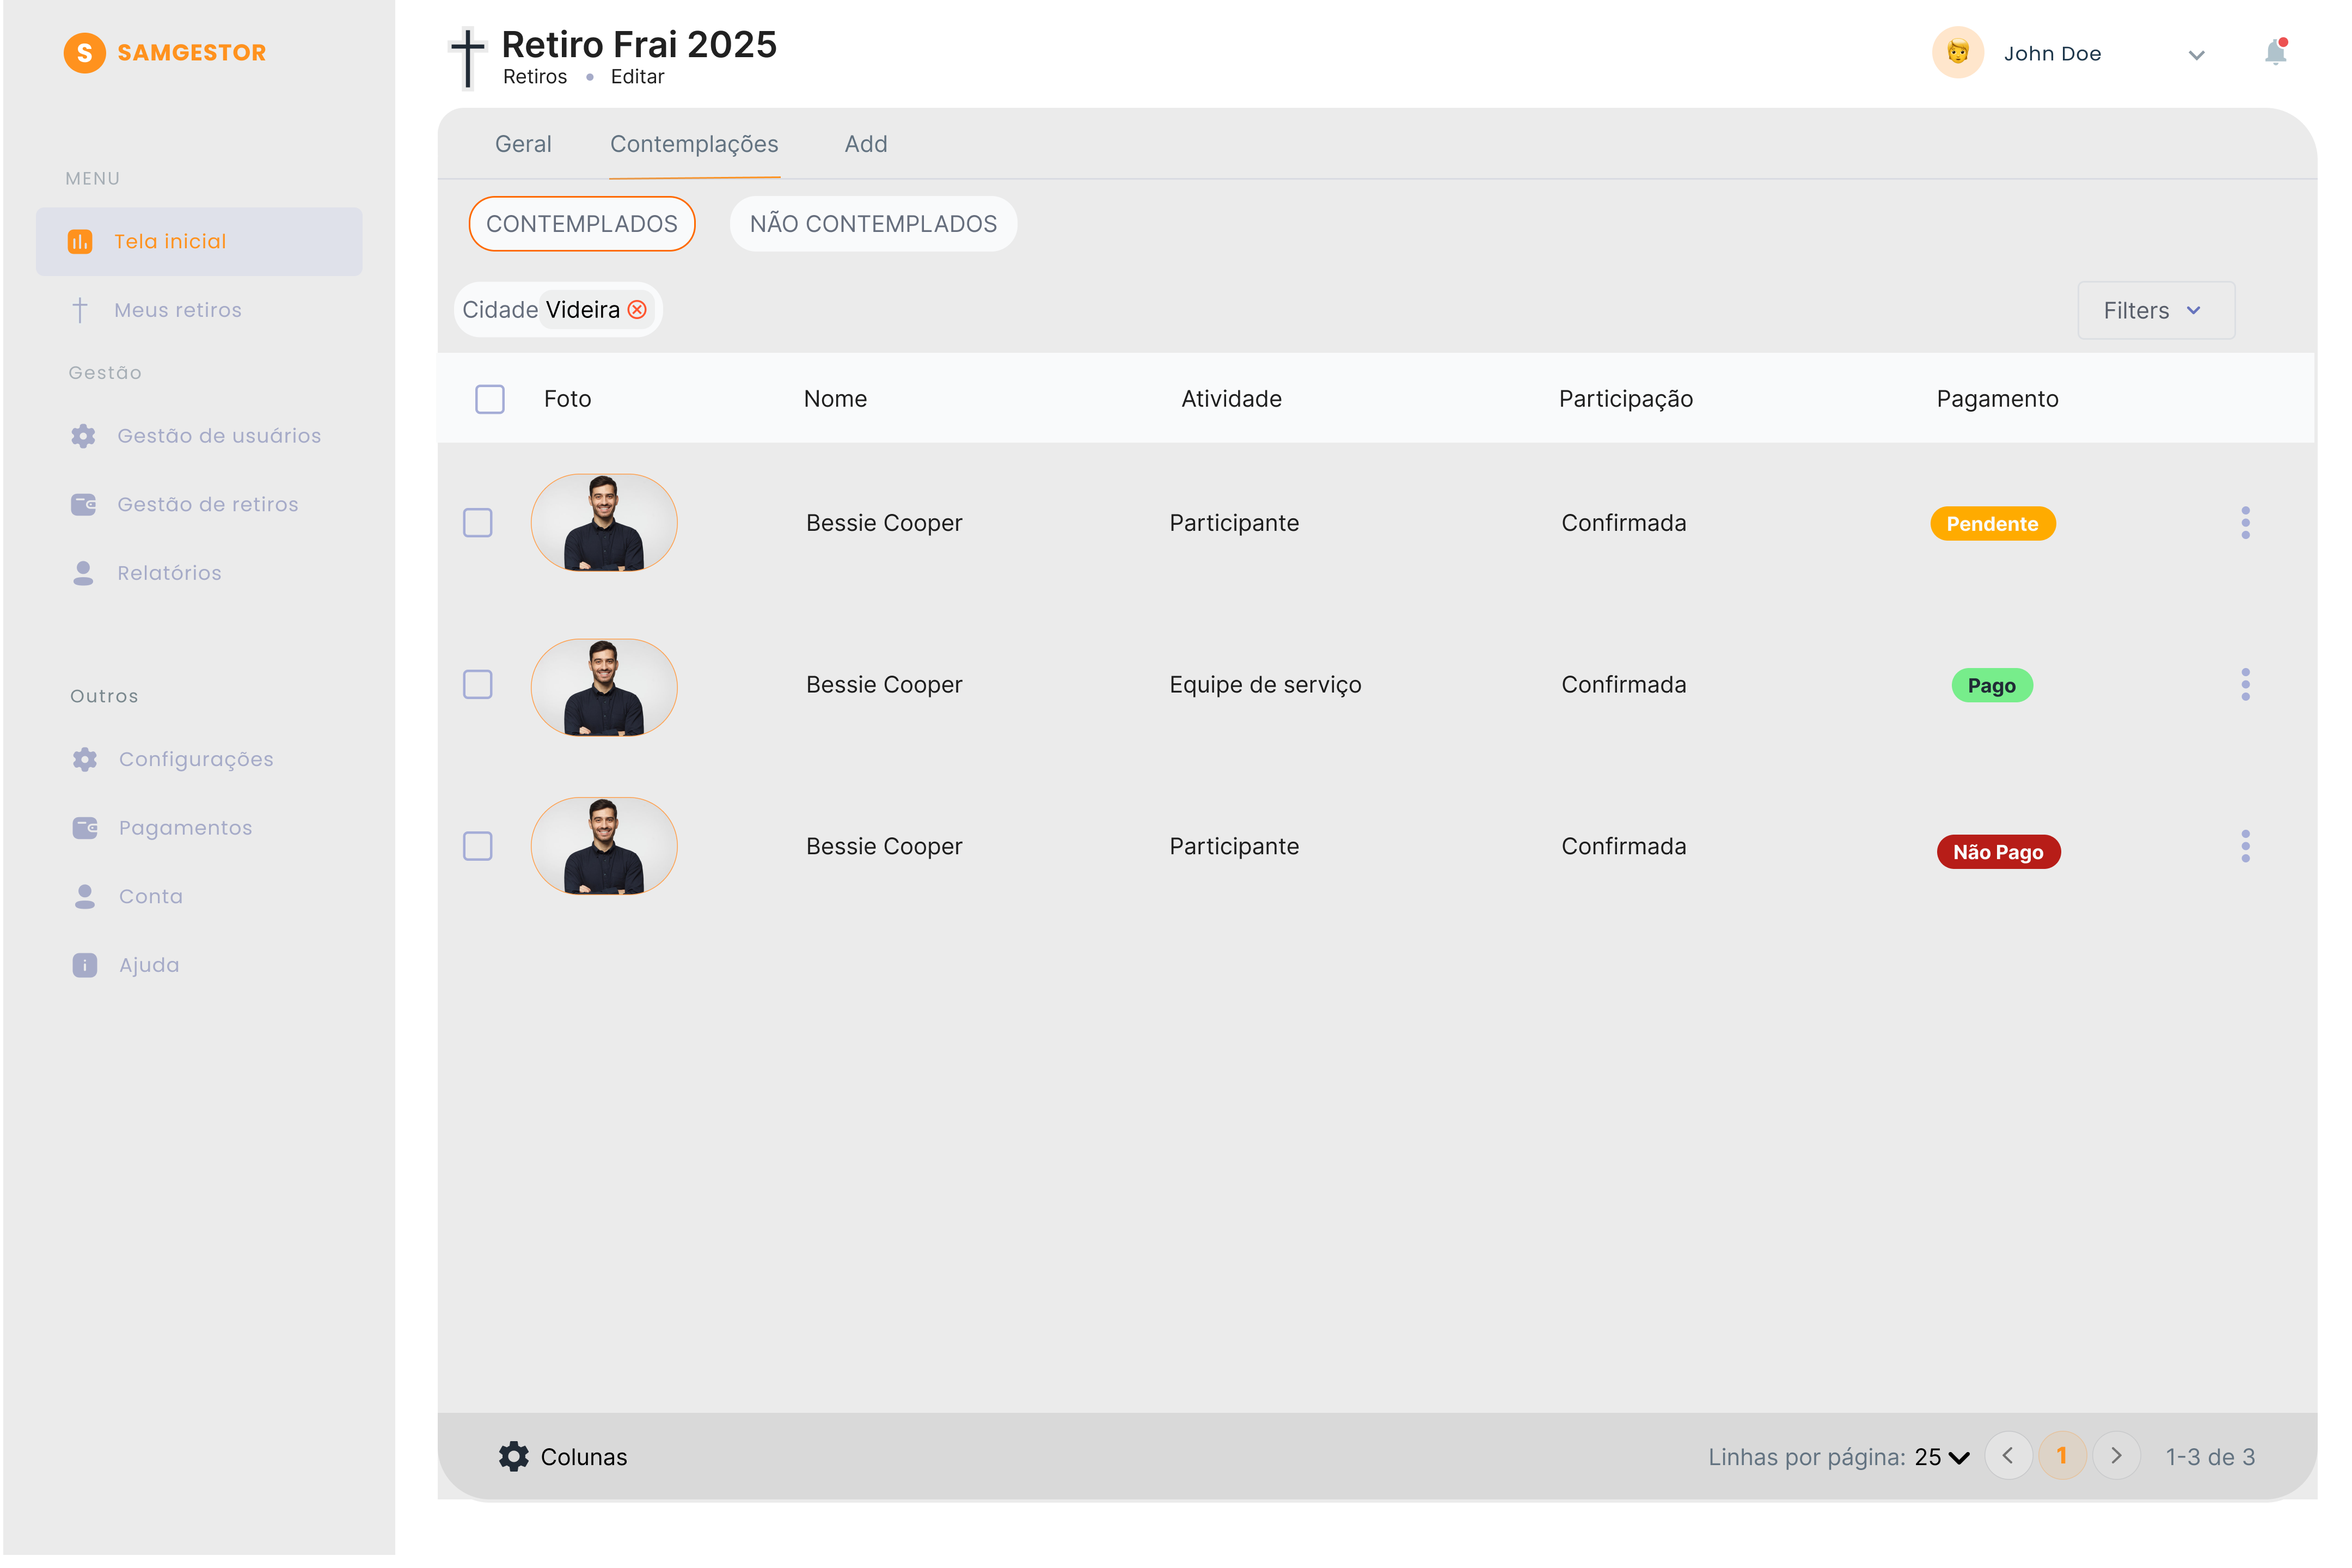
\includegraphics[width=0.8\textwidth]{images/prototipacao/gestao_retiros_geral/Contemplados-1.png}
\caption{Tabela de participantes contemplados. Exibe a lista de participantes já selecionados para o retiro. Por meio do menu de contexto (acesso via clique com o botão direito do mouse), o gestor pode abrir o modal de envio de mensagem ou visualizar informações detalhadas do participante.}
\end{figure}

\begin{figure}[H]
\centering
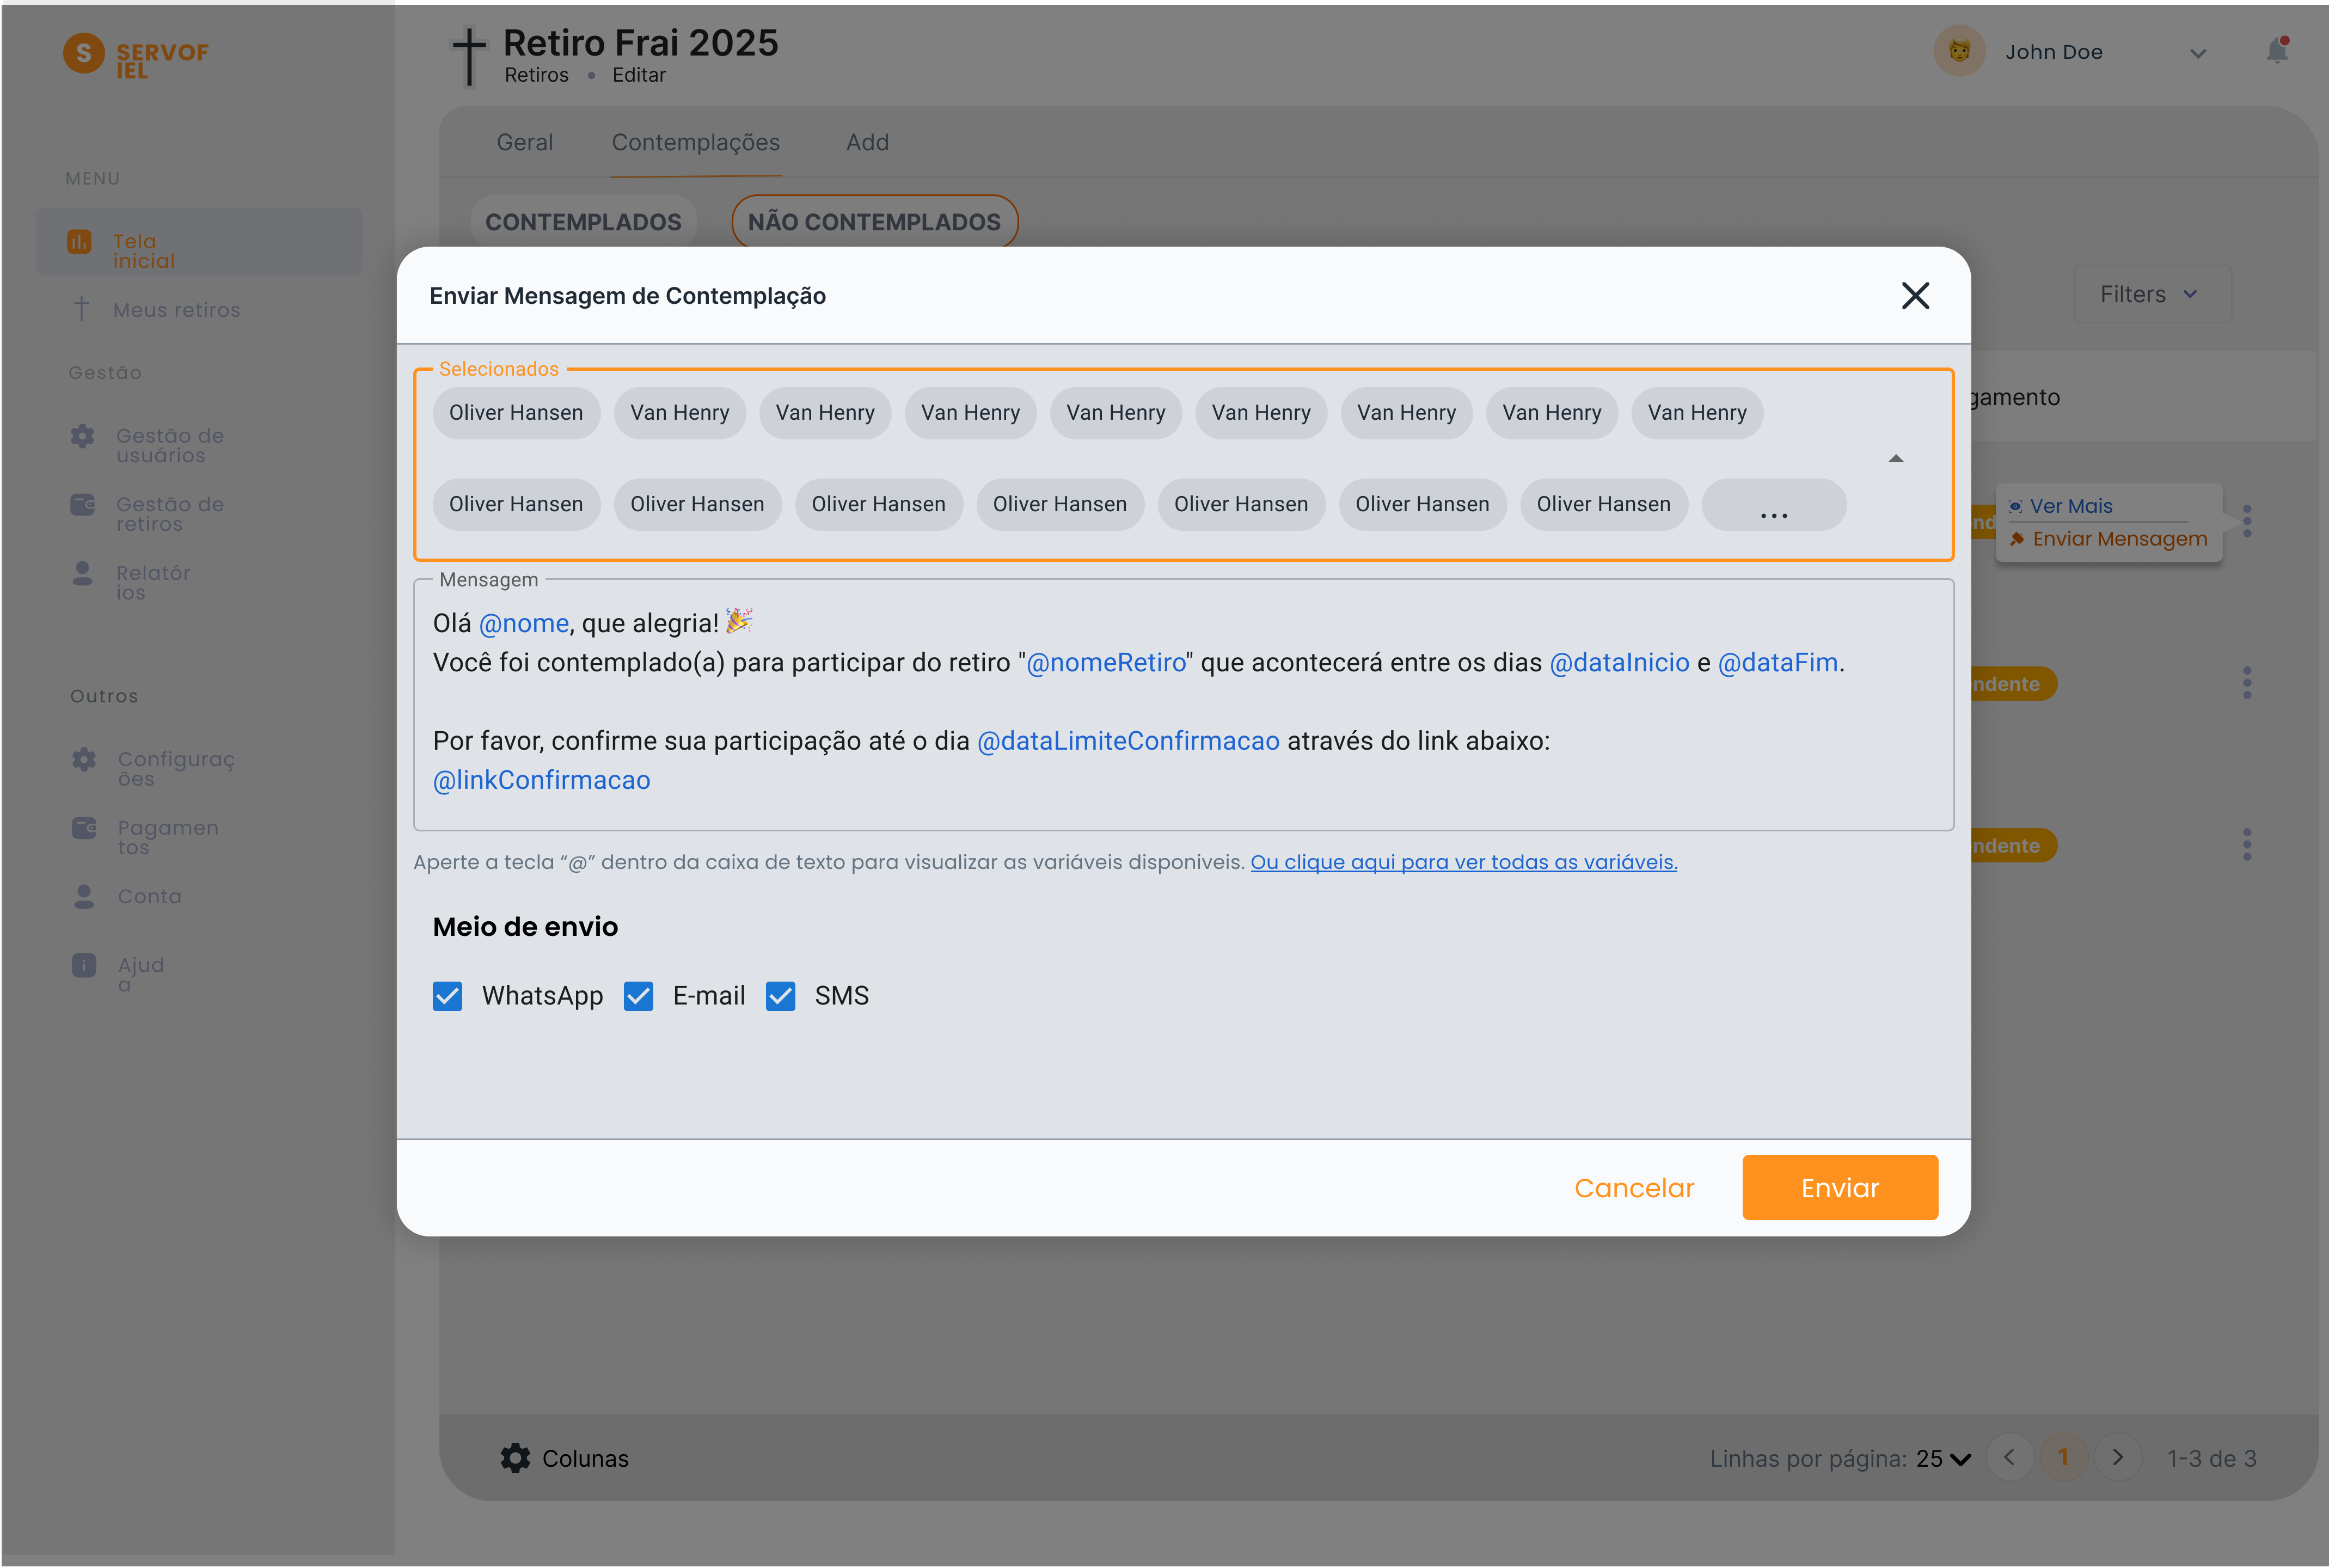
\includegraphics[width=0.8\textwidth]{images/prototipacao/gestao_retiros_geral/ContemplaçãoModal.png}
\caption{Modal de envio de mensagens personalizadas. Permite ao gestor compor e enviar mensagens personalizadas para participantes contemplados, com suporte ao envio em lote para múltiplos destinatários simultaneamente.}
\end{figure}

\begin{figure}[H]
\centering
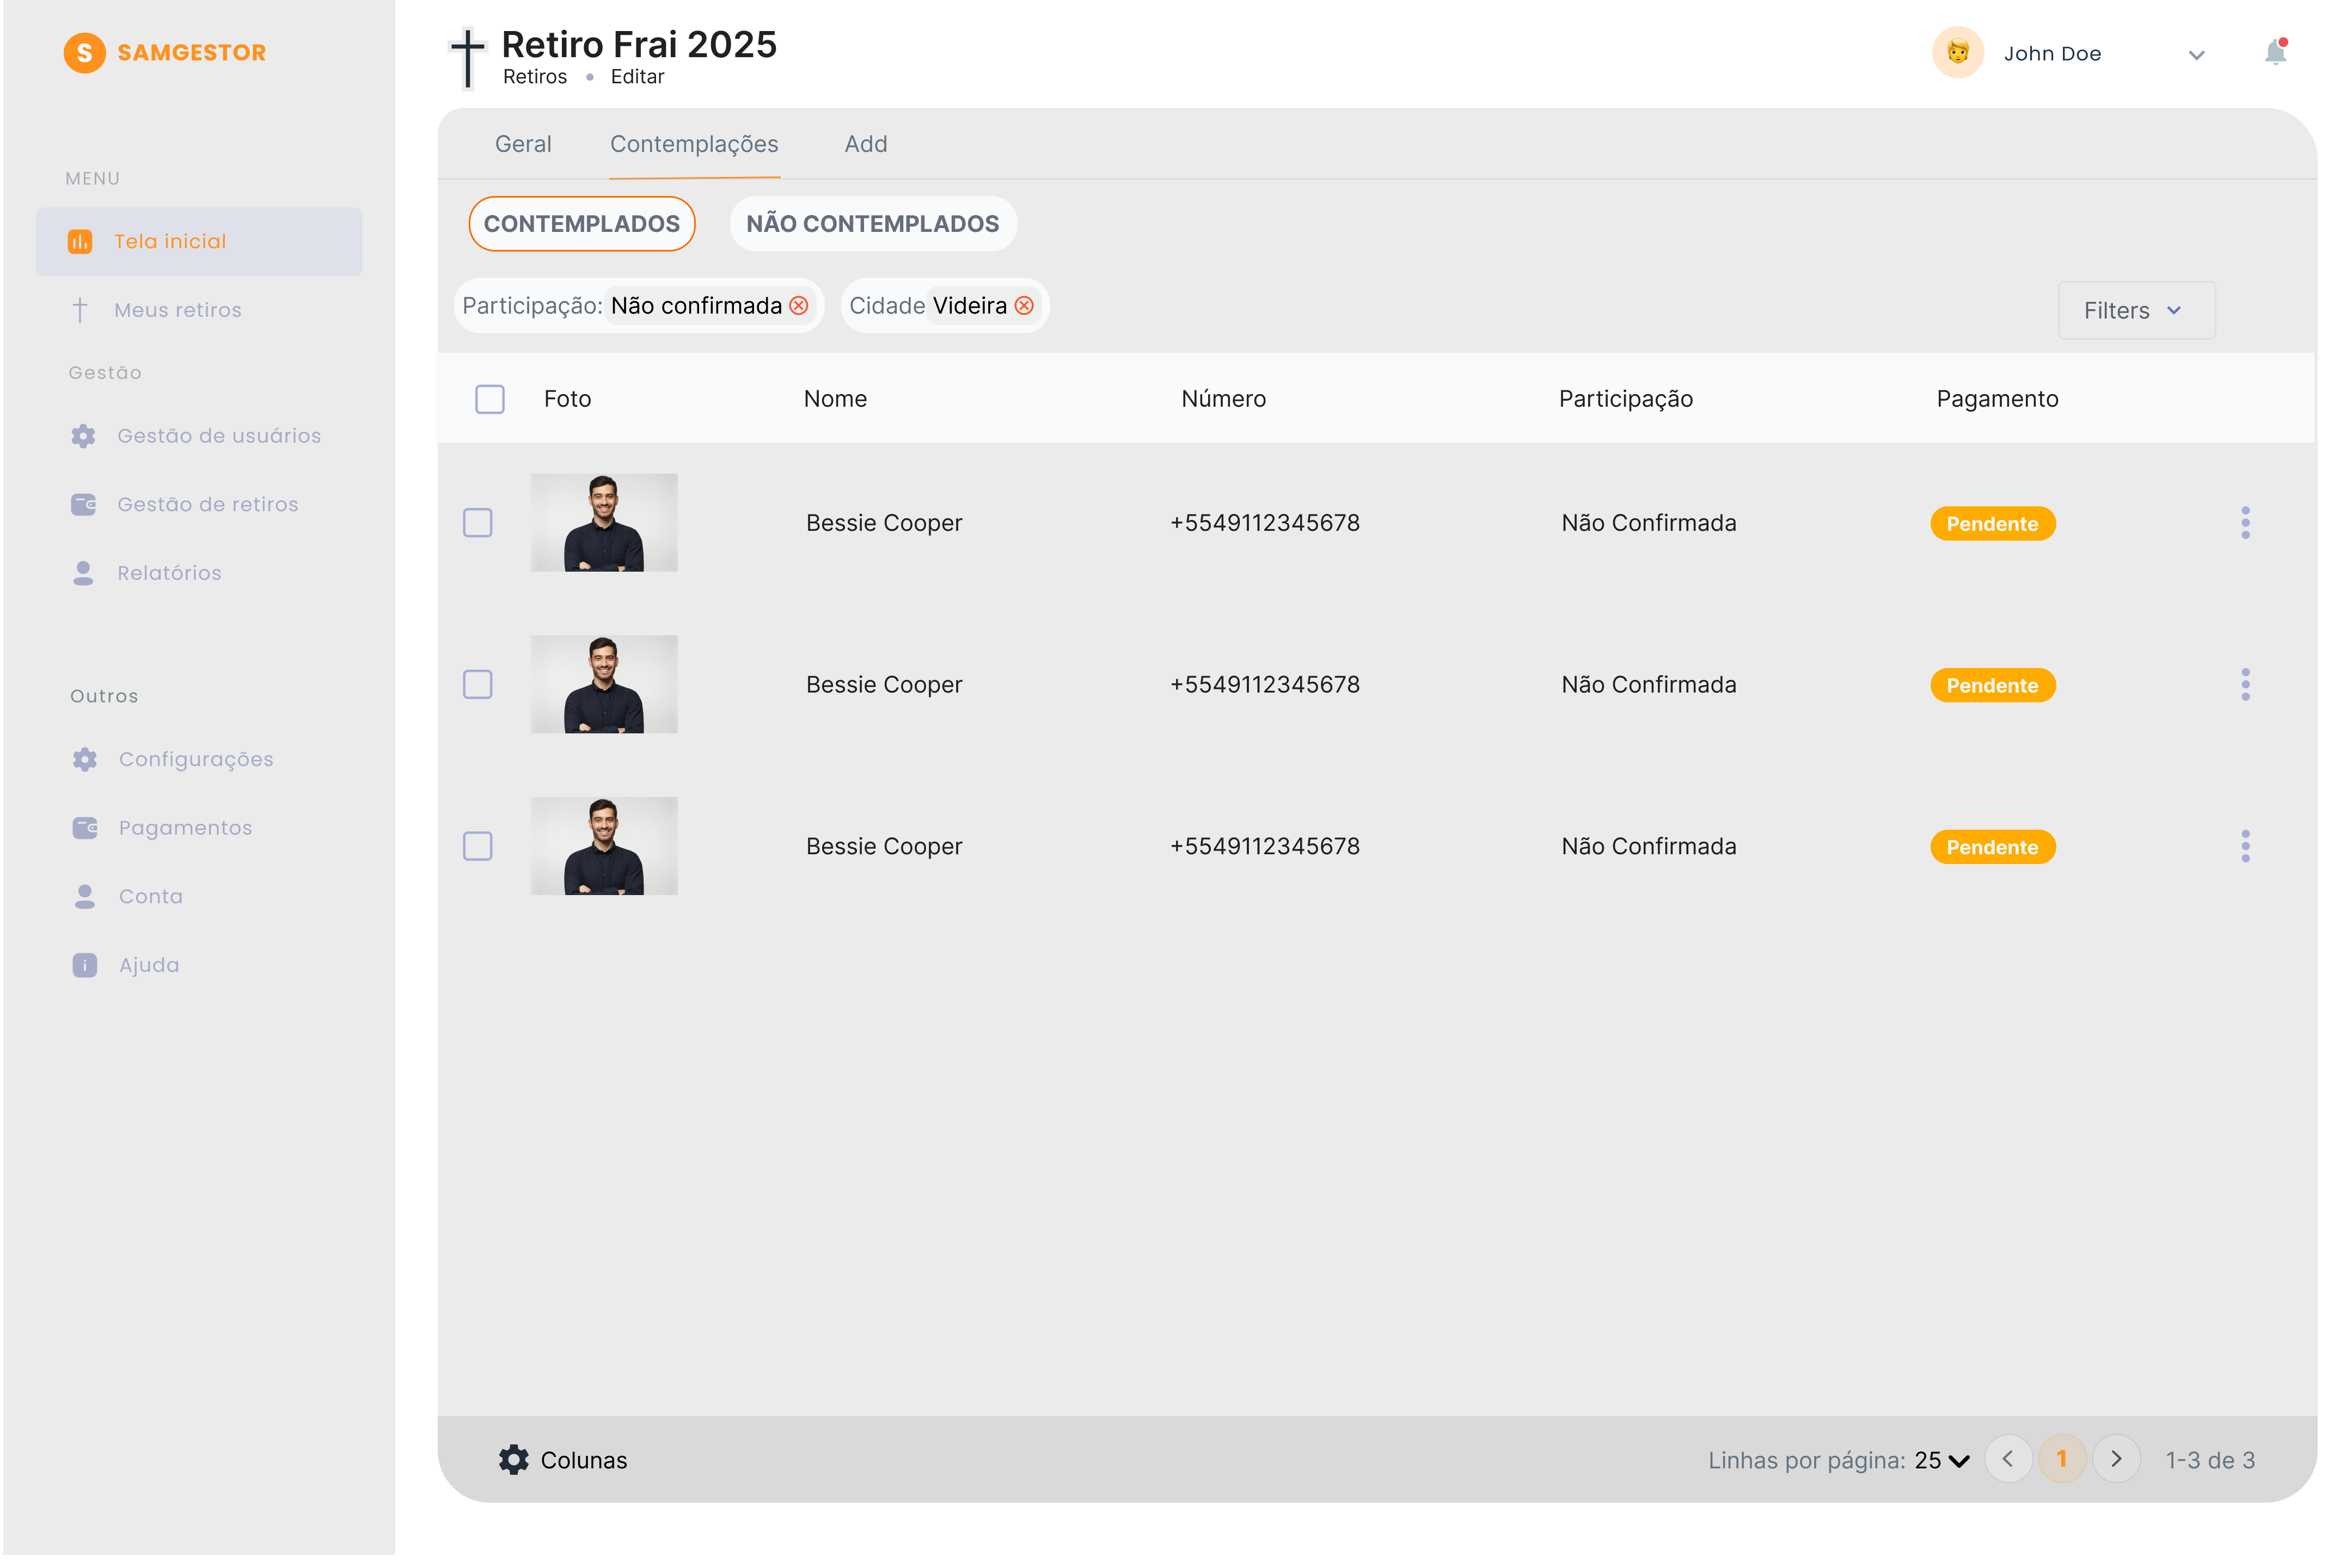
\includegraphics[width=0.8\textwidth]{images/prototipacao/gestao_retiros_geral/Pendentes.png}
\caption{Tabela com participantes contemplados com filtro de participação não confirmada.}
\end{figure}

\begin{figure}[H]
\centering
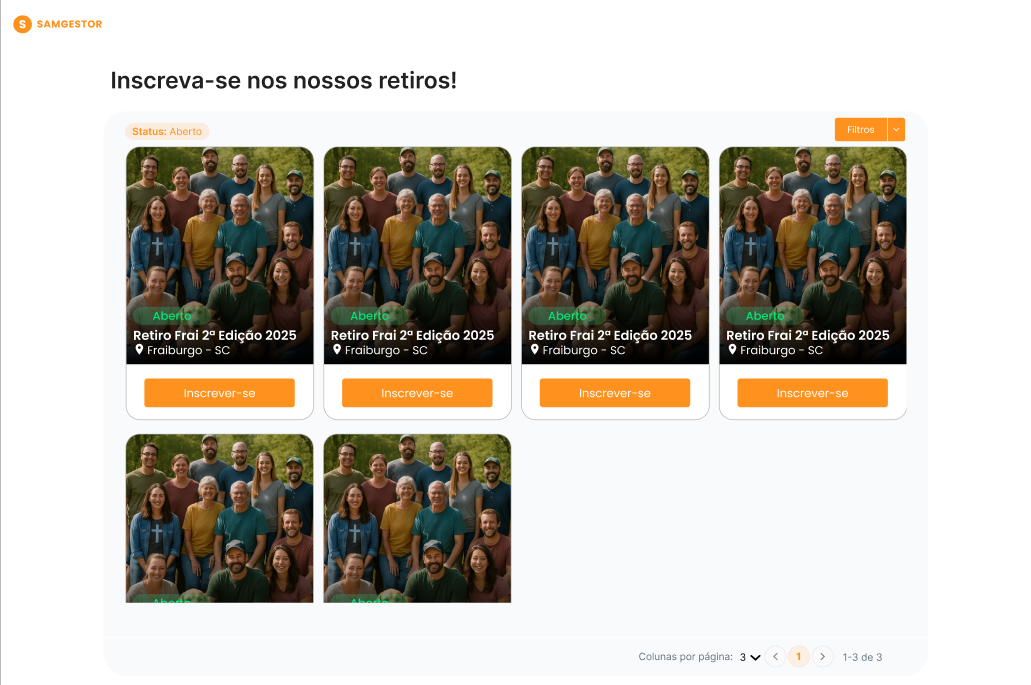
\includegraphics[width=0.8\textwidth]{images/prototipacao/form_publico/listVierPage.png}
\caption{Página inicial com os retiros.}
\end{figure}

\begin{figure}[H]
\centering
\includegraphics[width=0.8\textwidth]{images/prototipacao/form_publico/Detail Page - Retiro.png}
\caption{Página com os detalhes do retiro e o formulário.}
\end{figure}

\begin{figure}[H]
\centering
\includegraphics[width=0.8\textwidth]{images/prototipacao/form_publico/Detail Page - Retiro (Success).png}
\caption{Mensagem de sucesso exibida após o envio do formulário. Informa ao usuário que o preenchimento foi concluído com êxito e os dados foram processados corretamente.}
\end{figure}

\begin{figure}[H]
\centering
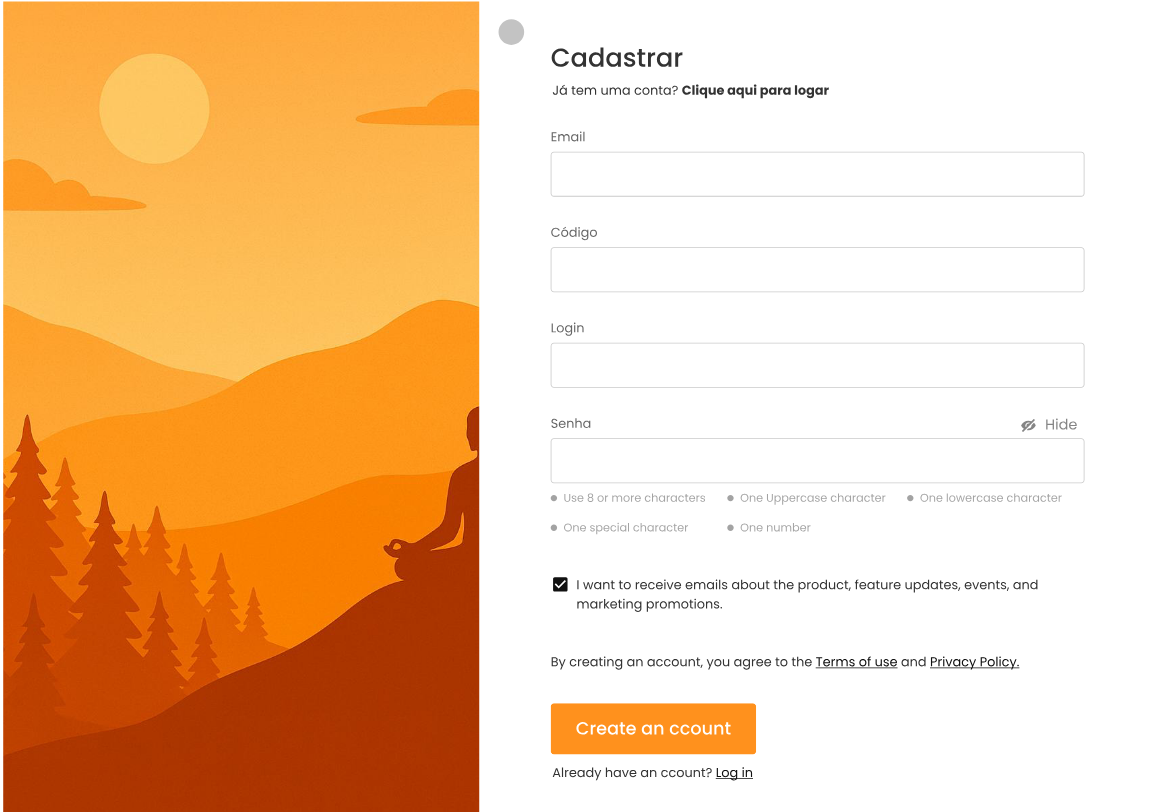
\includegraphics[width=0.8\textwidth]{images/prototipacao/participant_login/register.png}
\caption{Página de registro para participantes contemplados. Permite que o participante selecionado para o retiro crie sua conta de acesso ao sistema, inserindo suas informações pessoais e definindo suas credenciais de autenticação.}
\end{figure}

\begin{figure}[H]
\centering
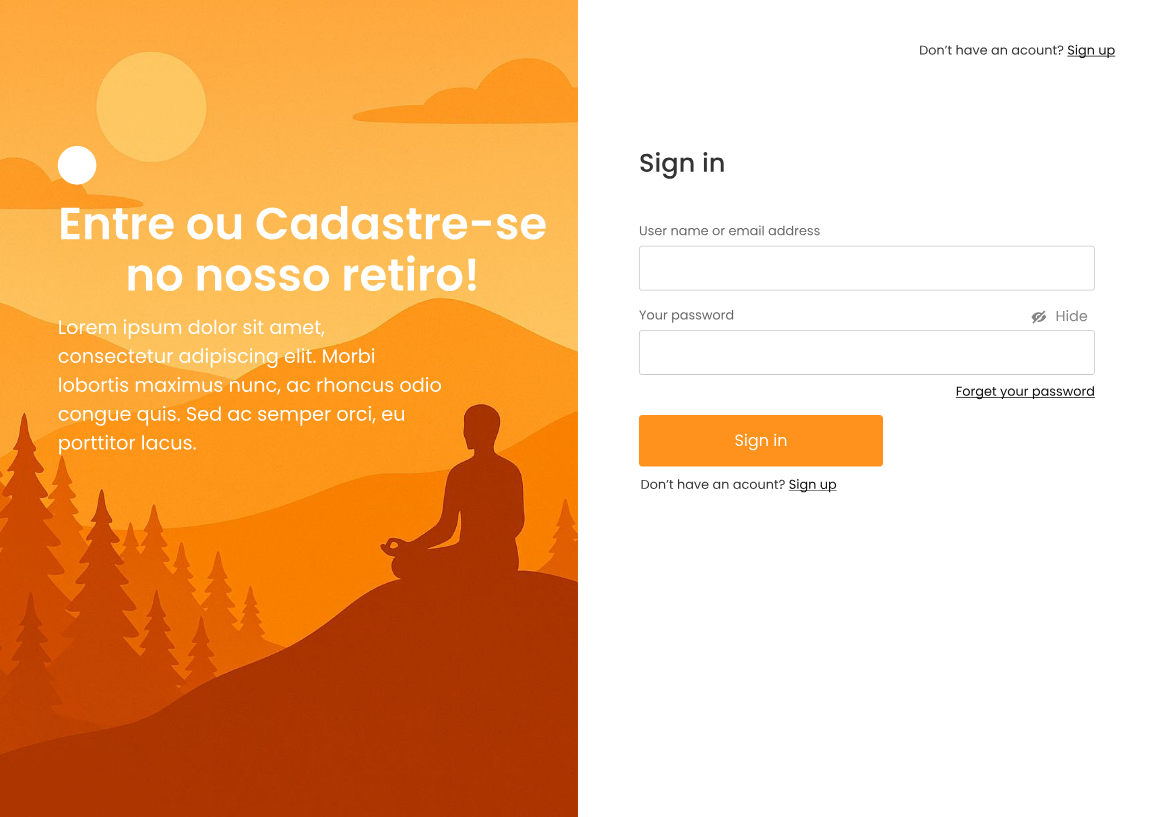
\includegraphics[width=0.8\textwidth]{images/prototipacao/participant_login/login.png}
\caption{Pagina de login geral dos usuários.}
\end{figure}

\begin{figure}[H]
    \centering
    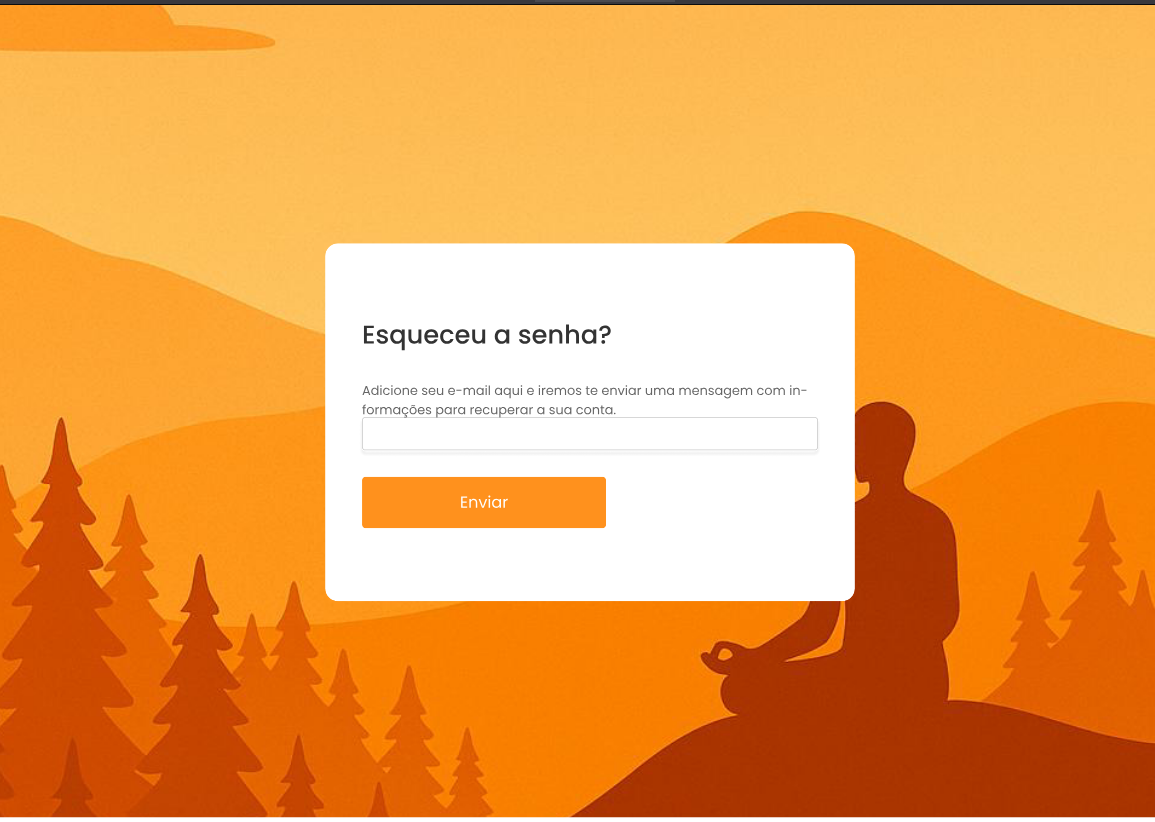
\includegraphics[width=0.8\textwidth]{images/prototipacao/participant_login/forgotpassword.png}
    \caption{Pagina de recuperacão das credenciais.}
    \end{figure}

\begin{figure}[H]
\centering
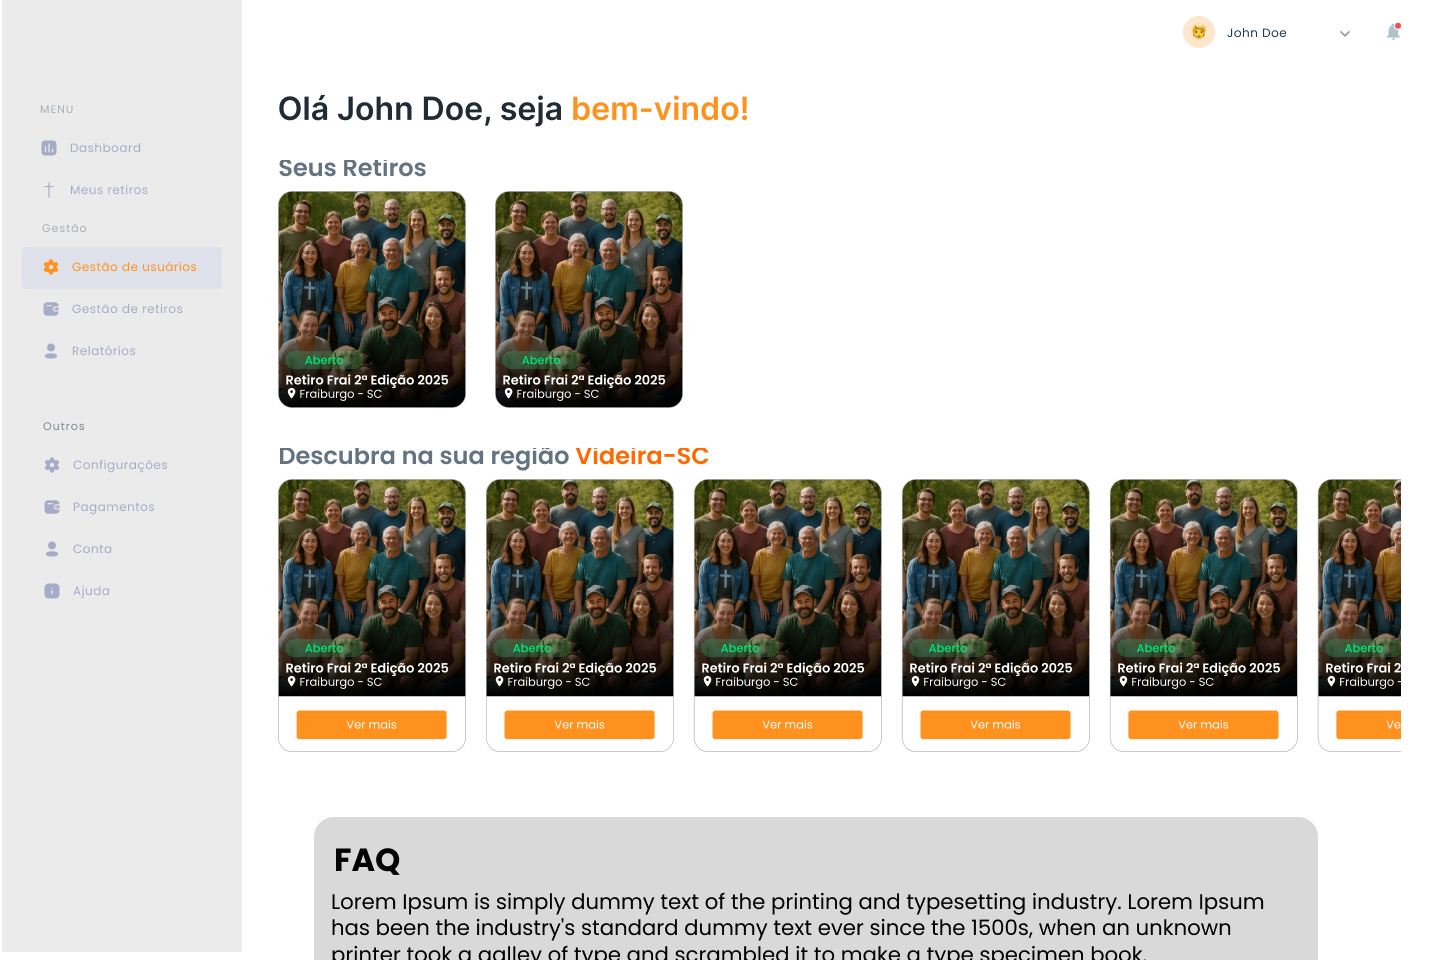
\includegraphics[width=0.8\textwidth]{images/prototipacao/participant_login/HomePage.png}
\caption{Paginá inicial do participante que irá pagar o retiro de forma automática.}
\end{figure}

\begin{figure}[H]
\centering
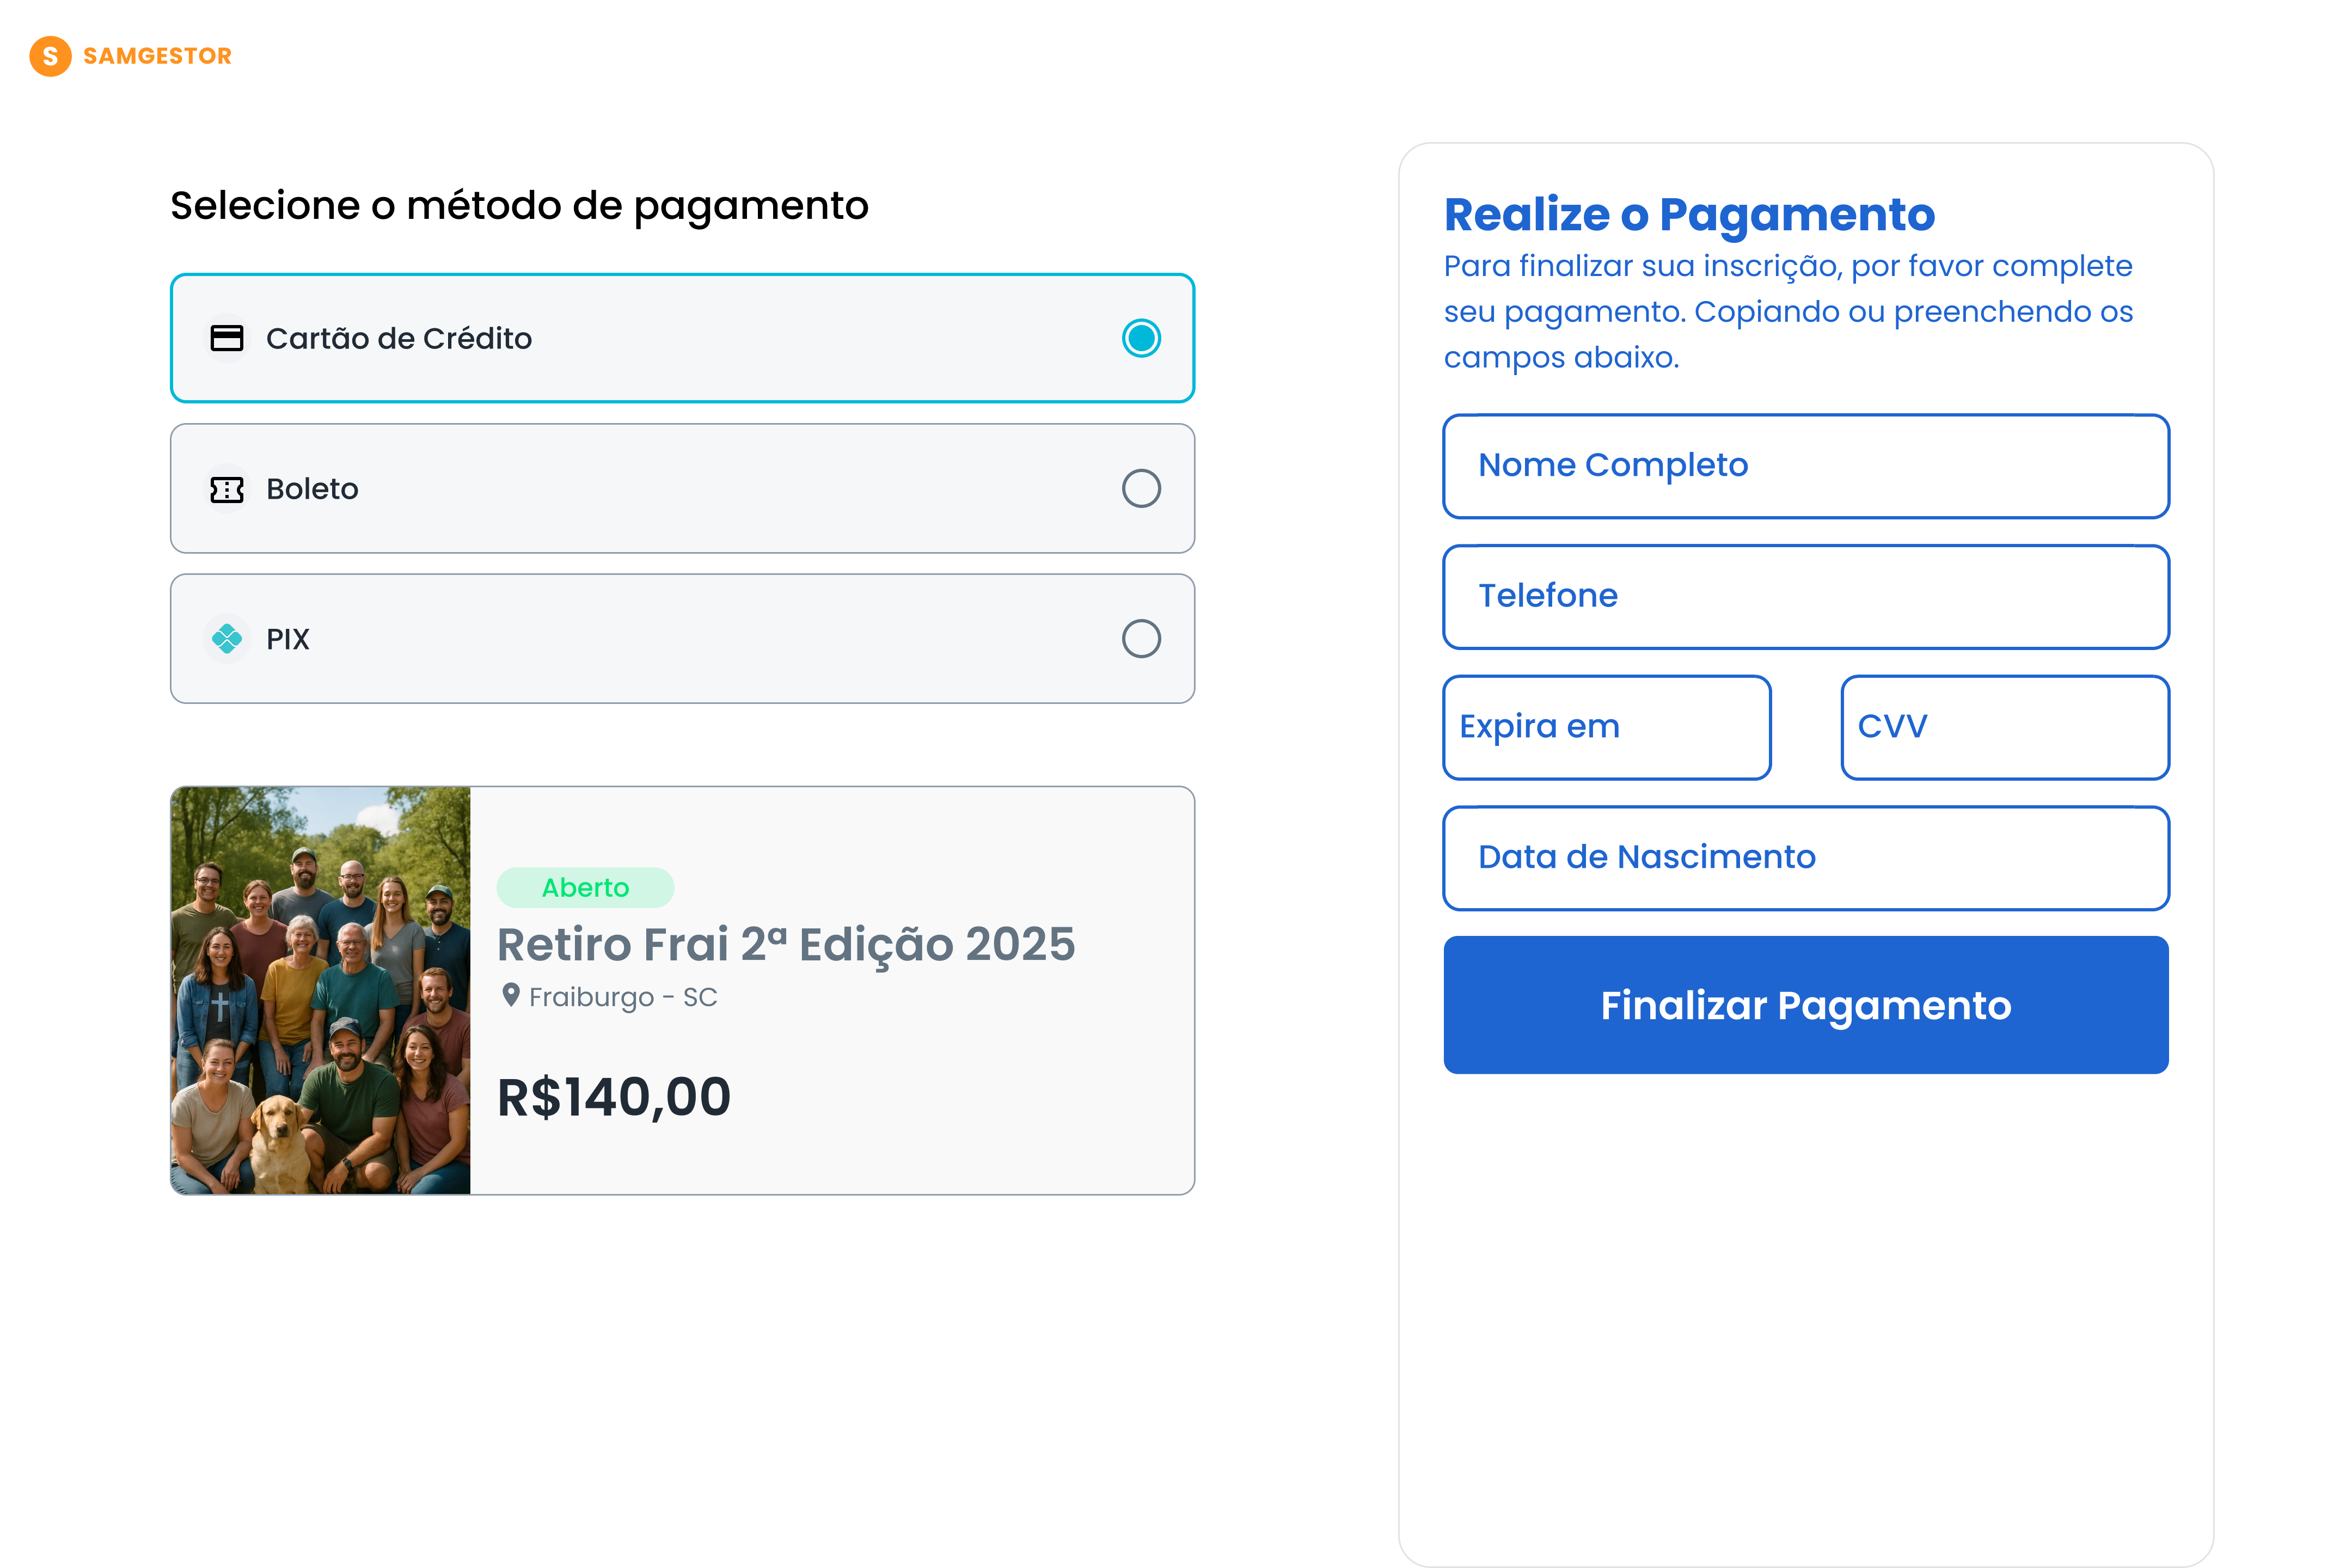
\includegraphics[width=0.8\textwidth]{images/prototipacao/participant_login/Payment Page - Retiro.png}
\caption{Escolha do pagamento no formato de crédito.}
\end{figure}

\begin{figure}[H]
\centering
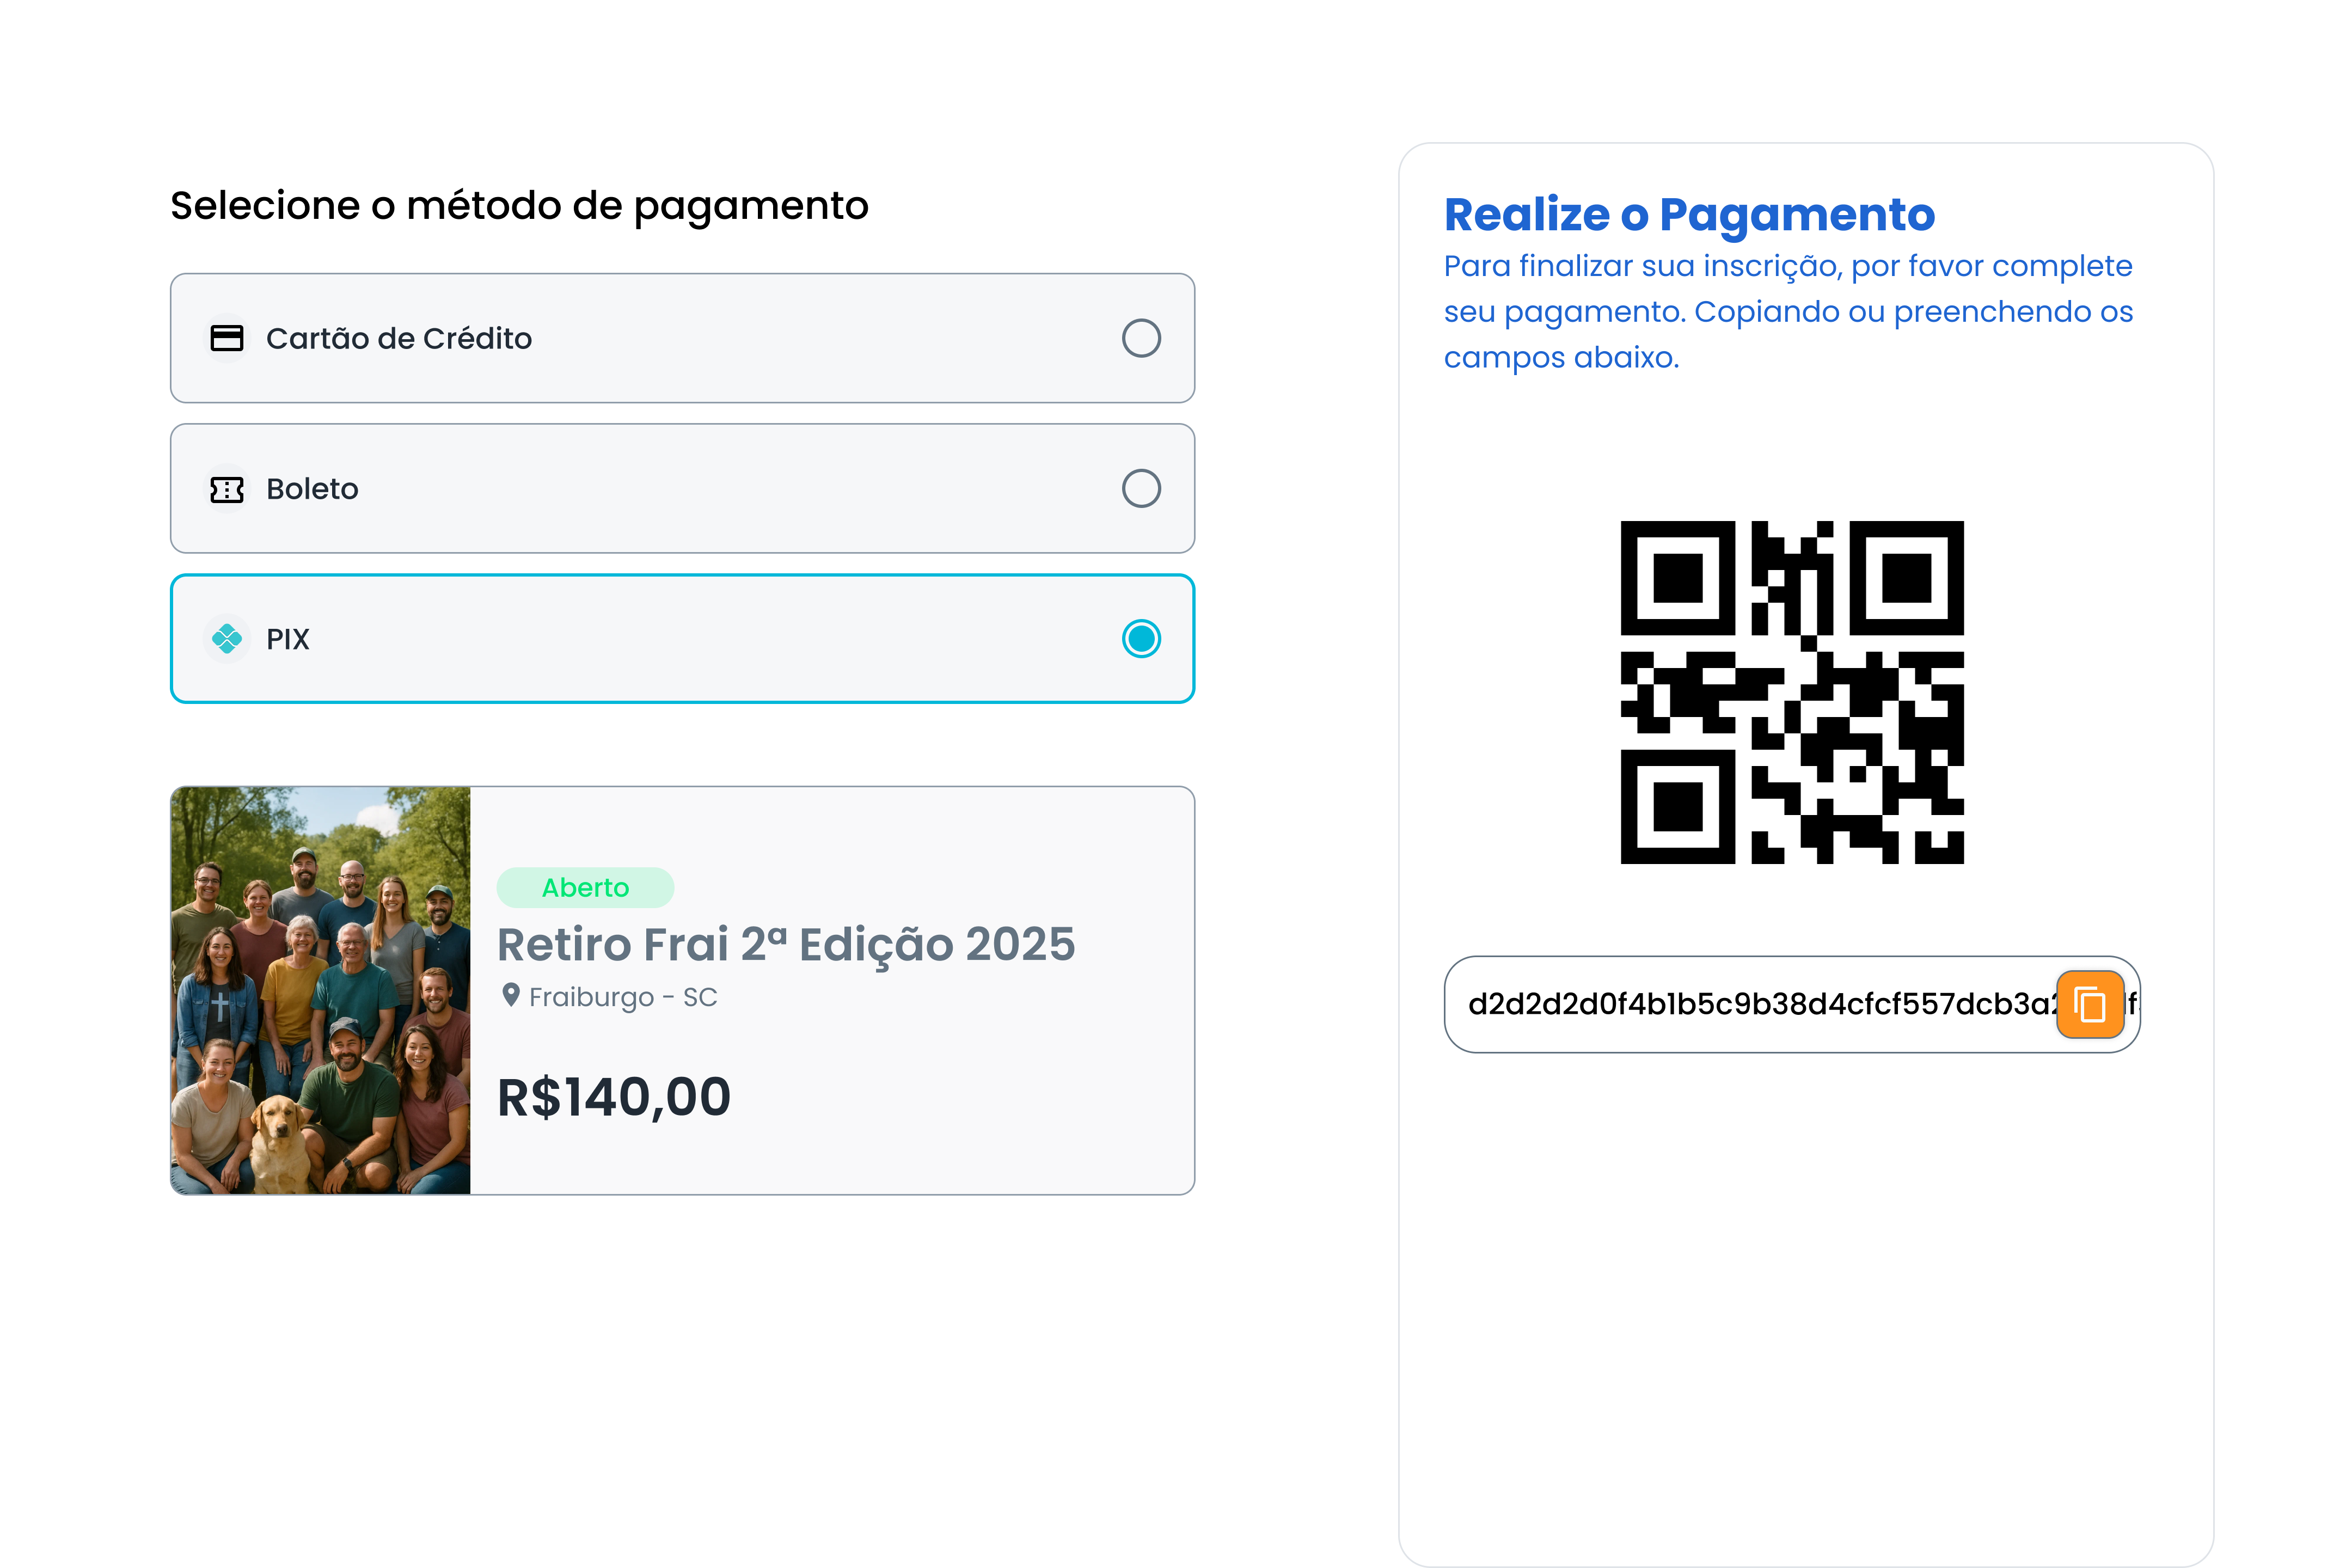
\includegraphics[width=0.8\textwidth]{images/prototipacao/participant_login/Payment Page - Retiro-1.png}
\caption{Escolha do pagamento no formato de PIX.}
\end{figure}


\begin{figure}[H]
\centering
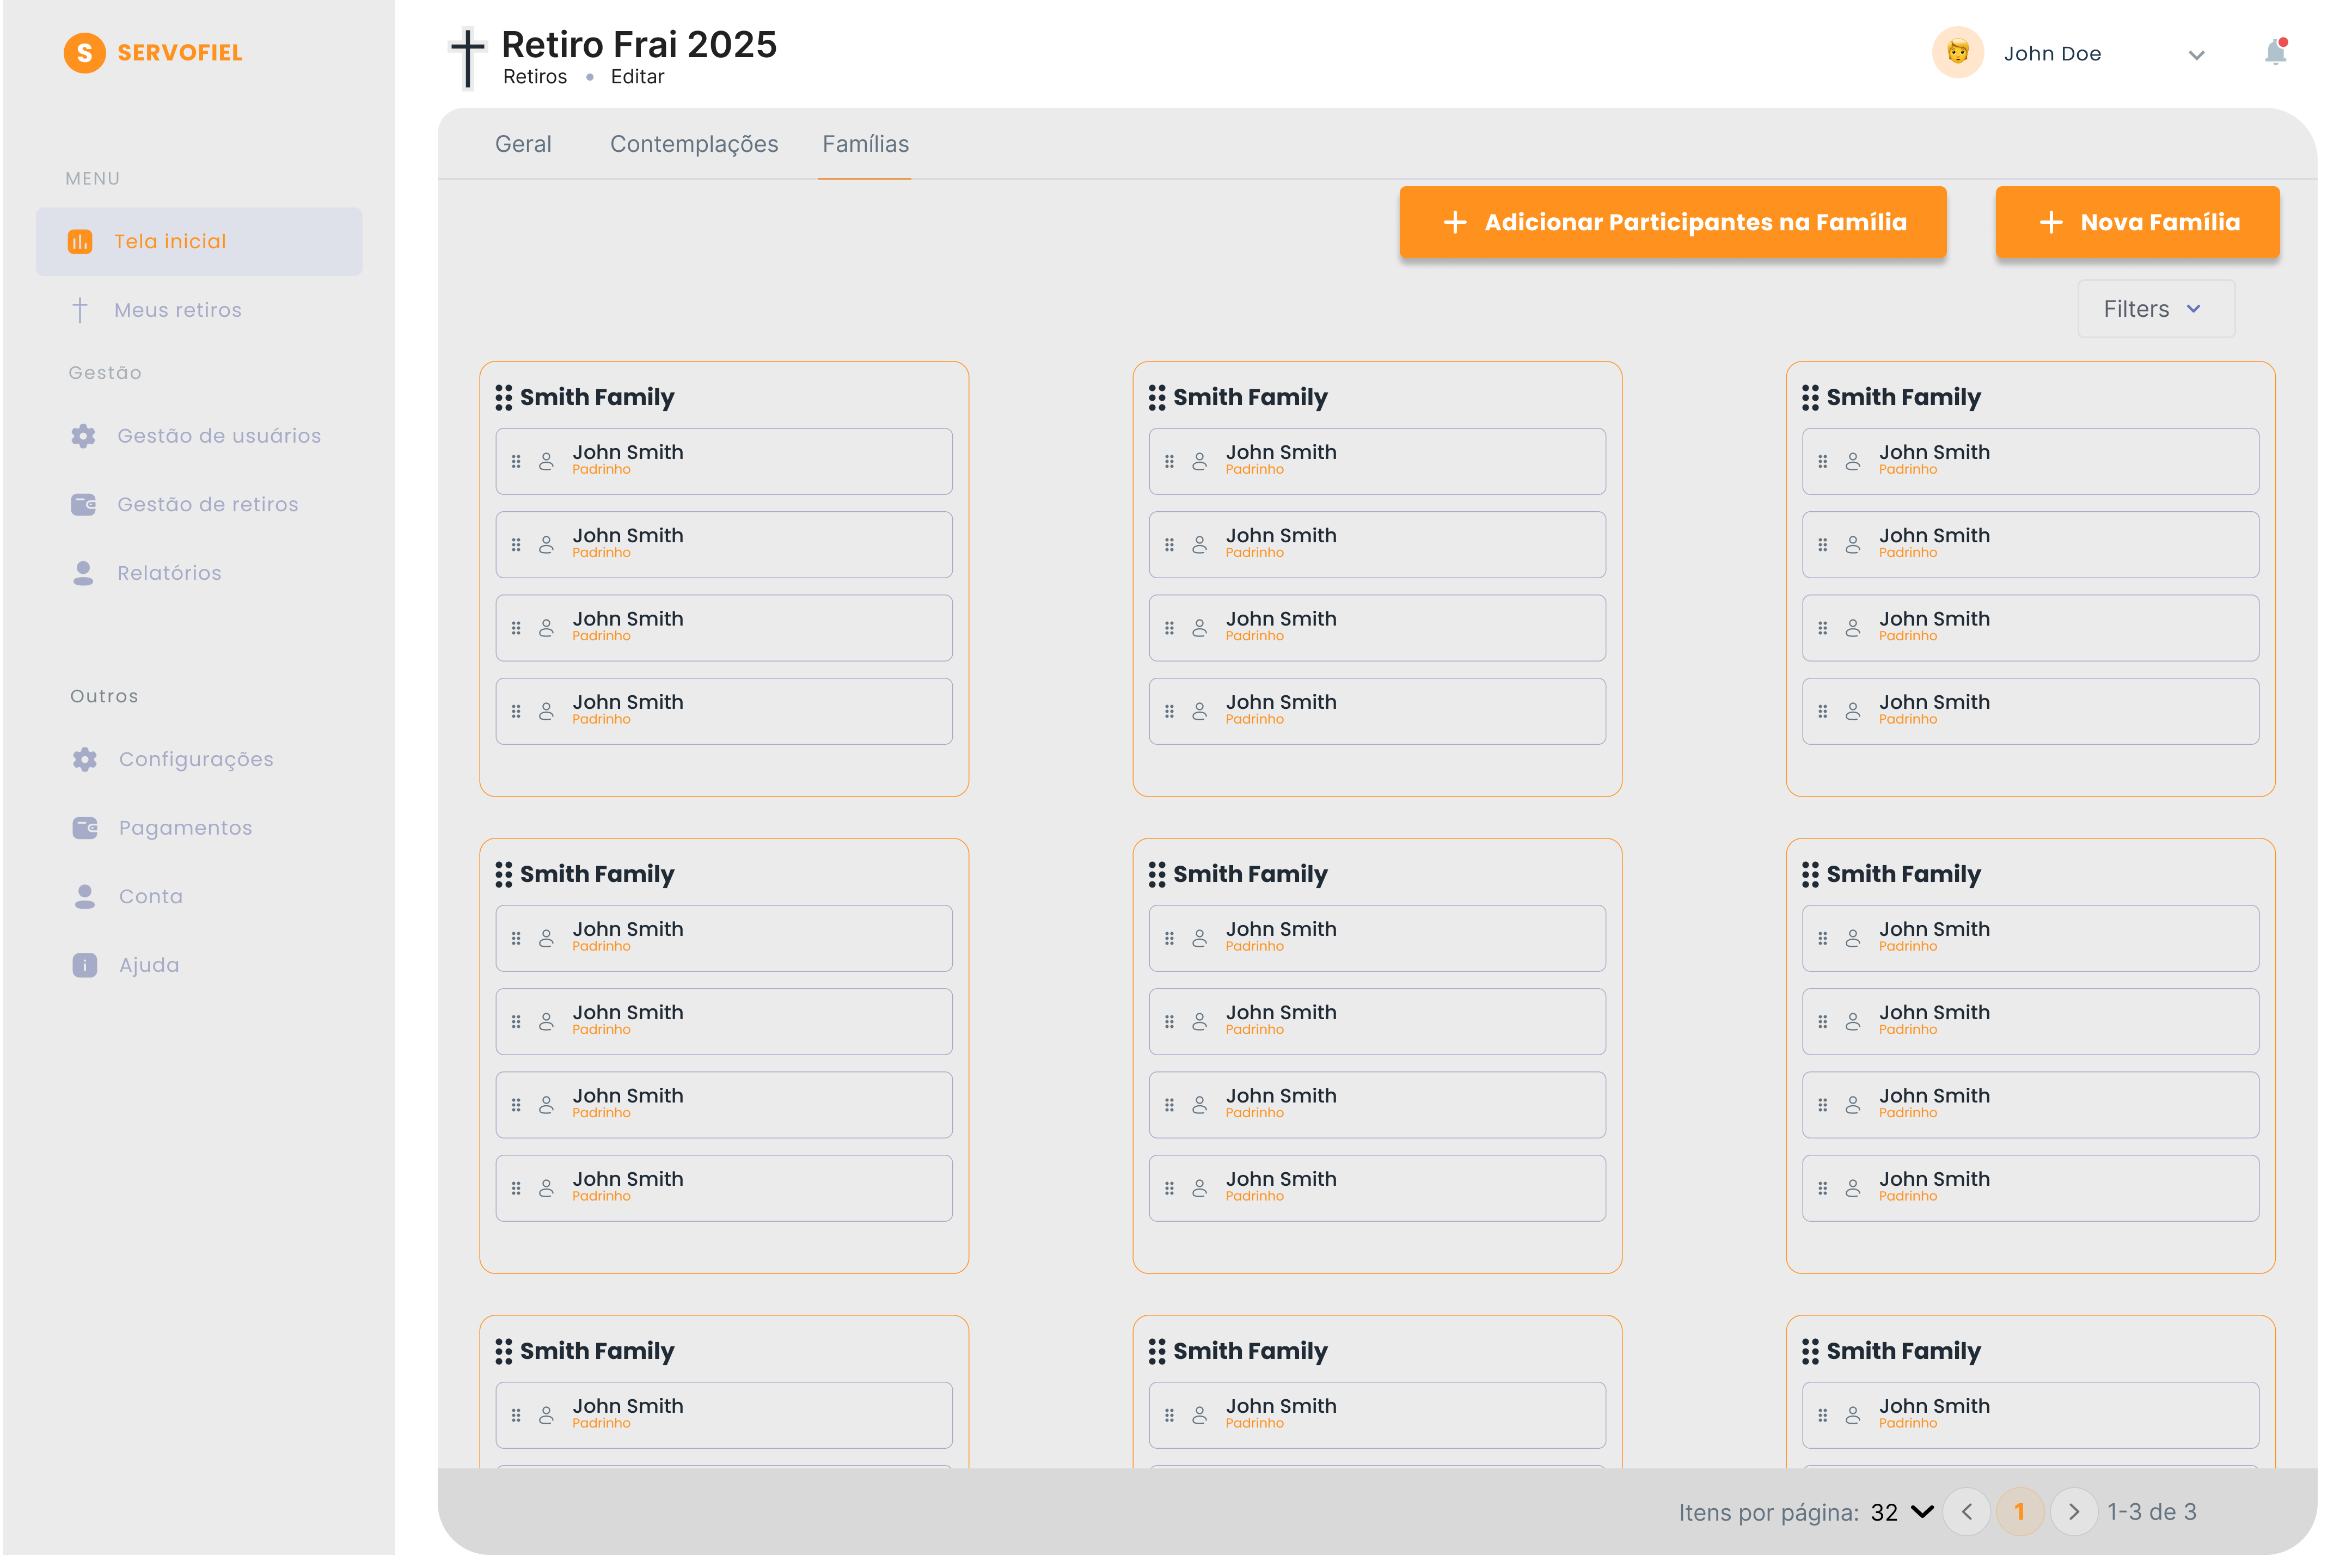
\includegraphics[width=0.8\textwidth]{images/prototipacao/familia/Familias-3.png}
\caption{Tela inicial das famílias.}
\end{figure}

\begin{figure}[H]
\centering
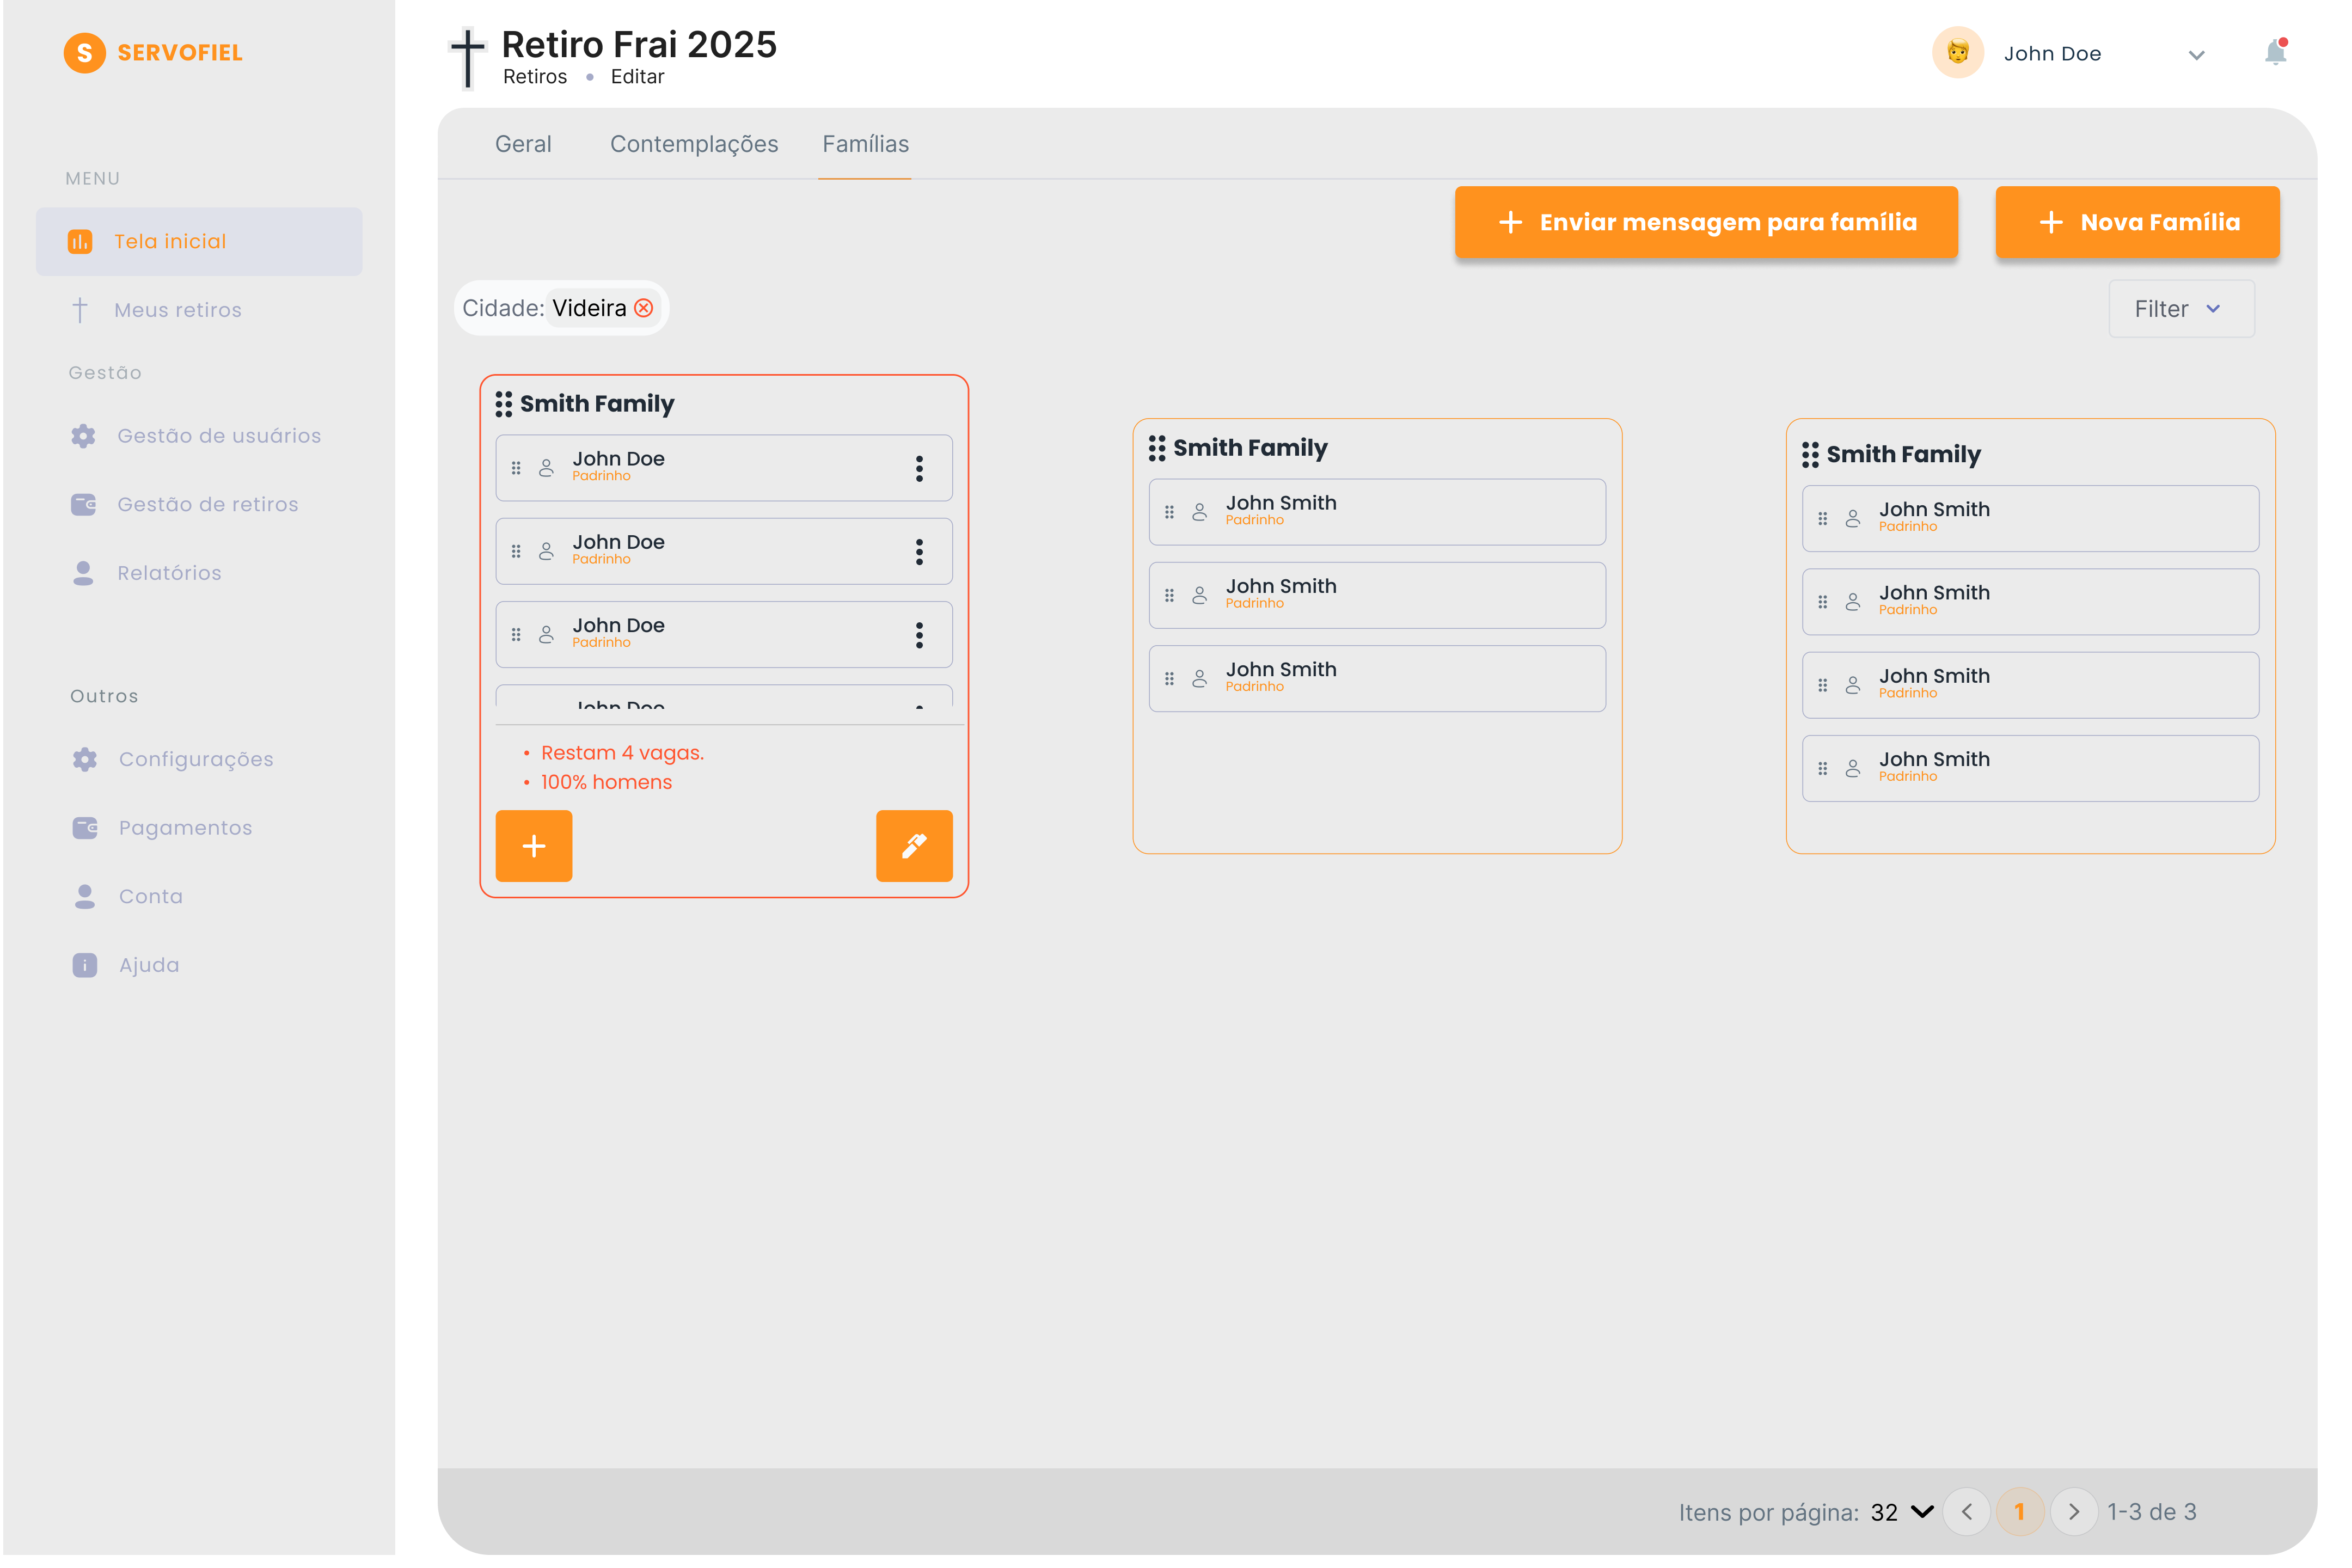
\includegraphics[width=0.8\textwidth]{images/prototipacao/familia/Familias-2.png}
\caption{Avisos de erros na composição de uma família.}
\end{figure}

\begin{figure}[H]
\centering
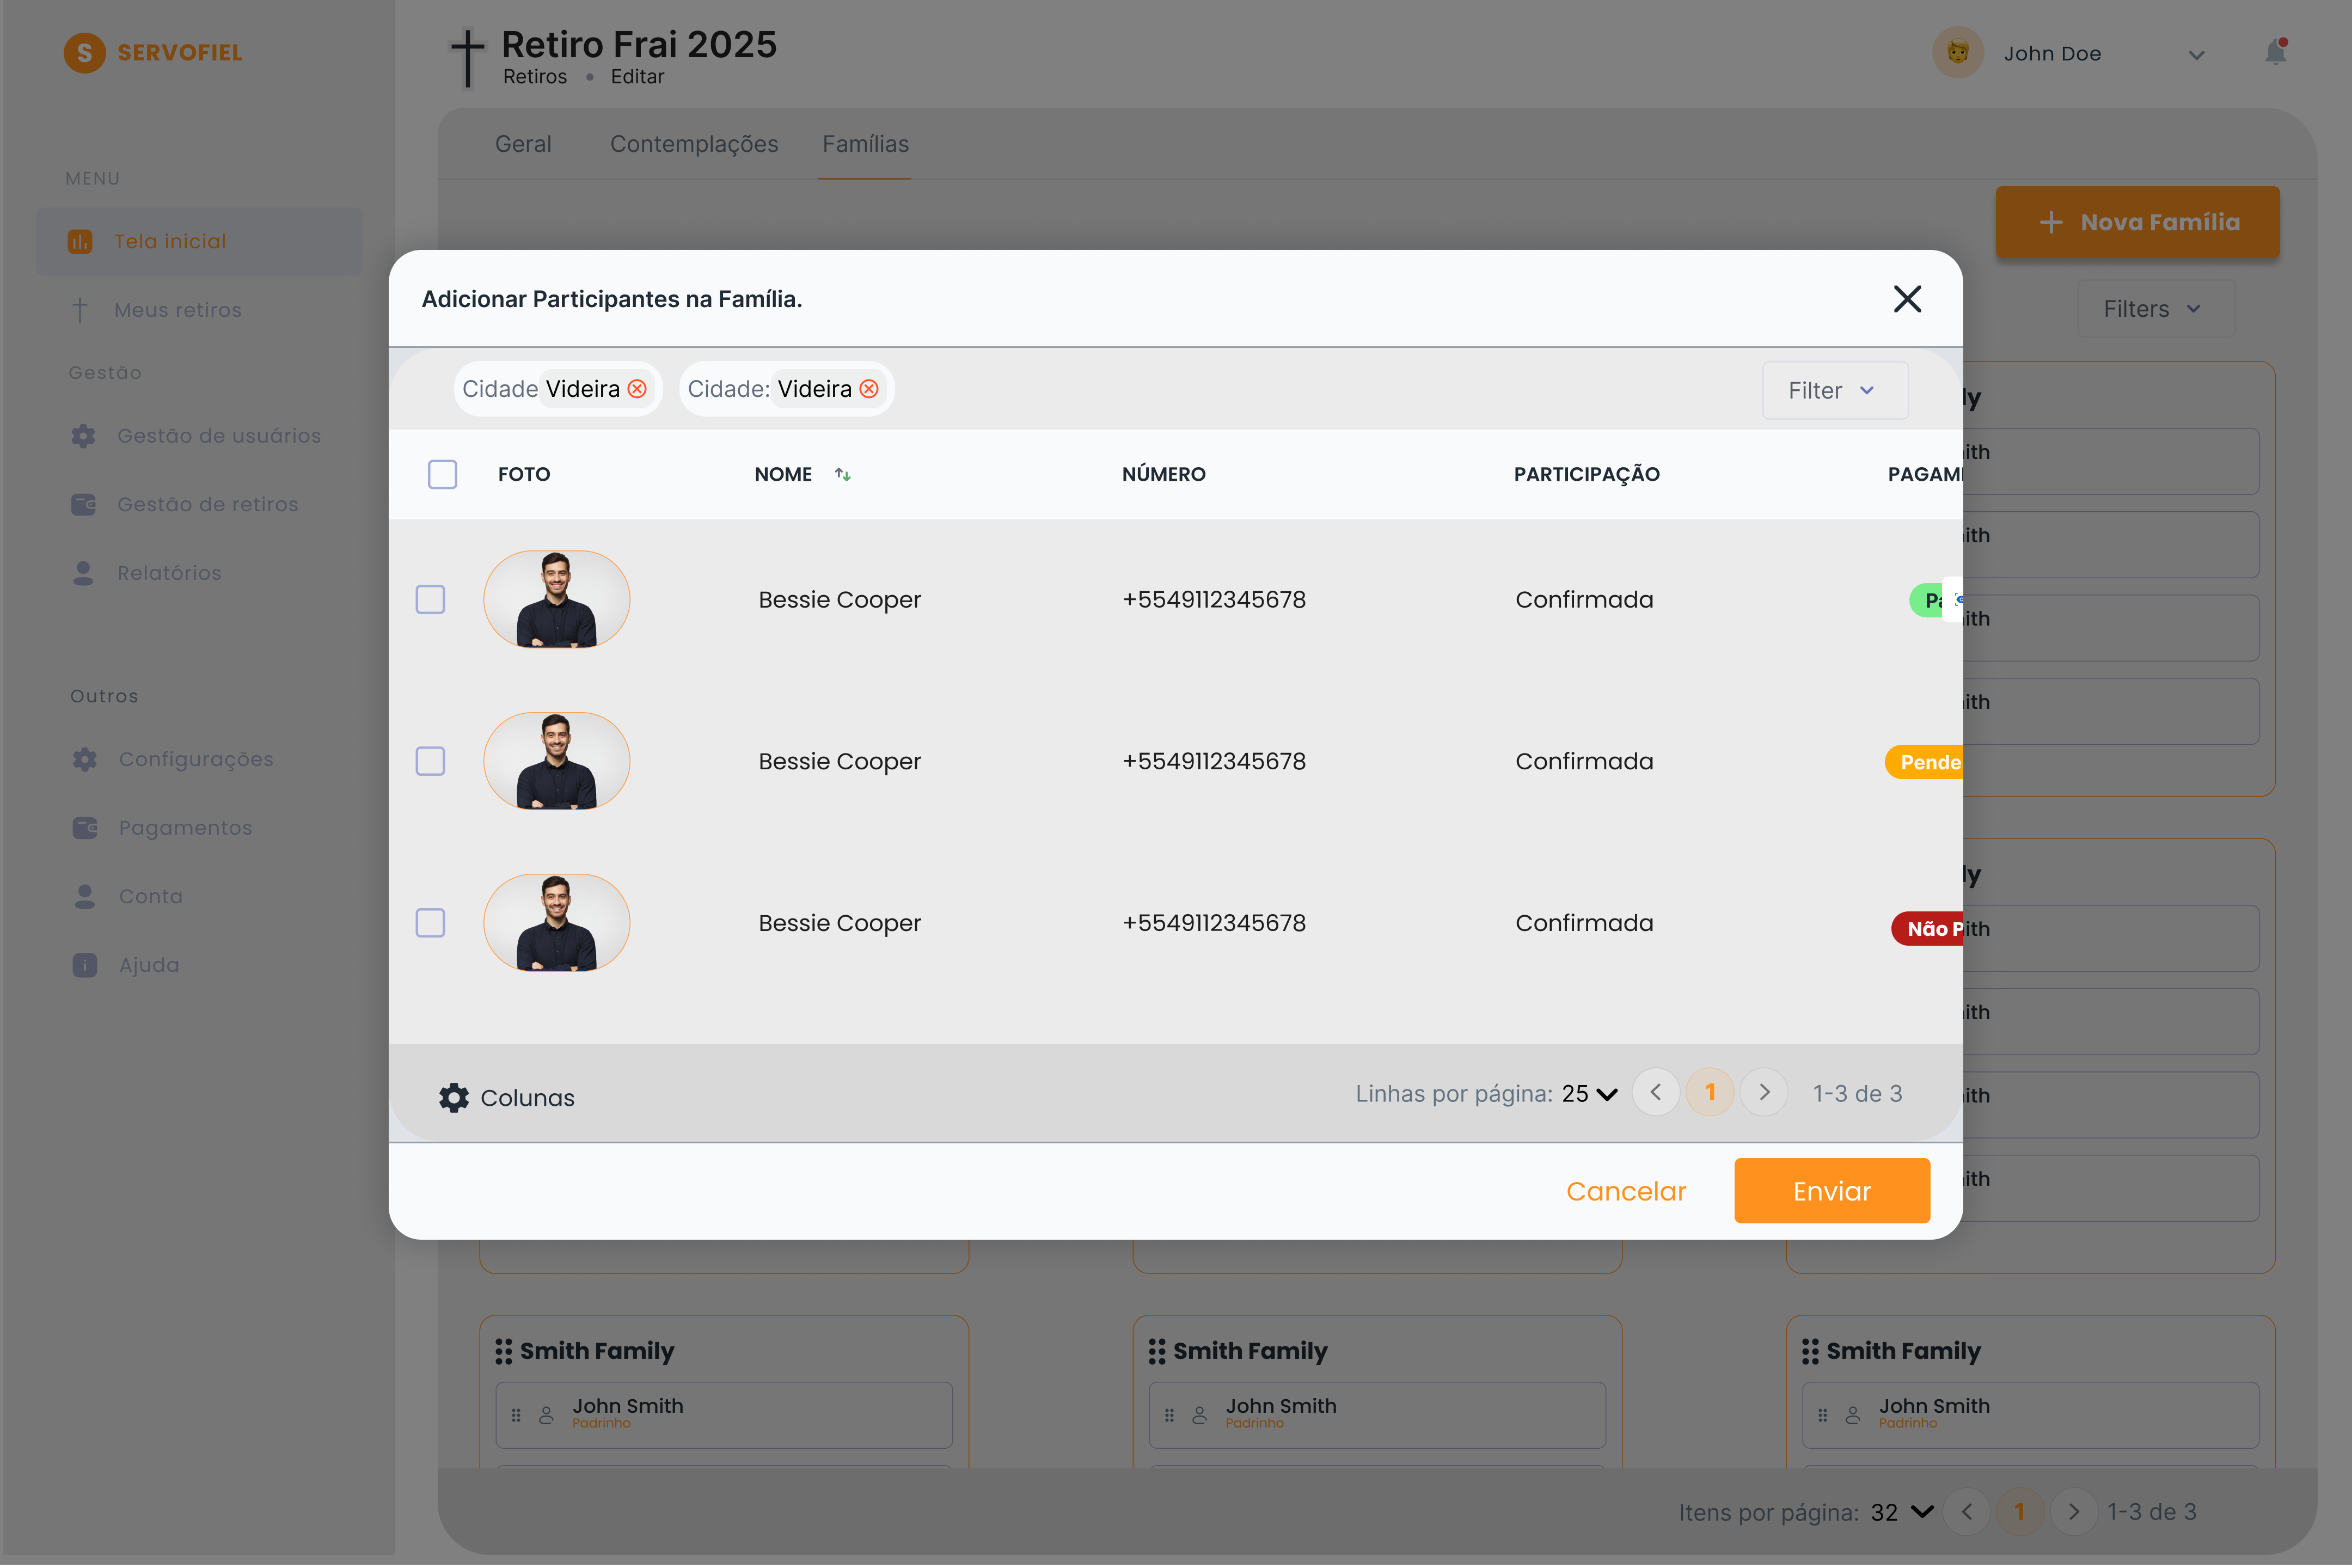
\includegraphics[width=0.8\textwidth]{images/prototipacao/familia/Familias-1.png}
\caption{Adição de um participante na família.}
\end{figure}

\begin{figure}[H]
\centering
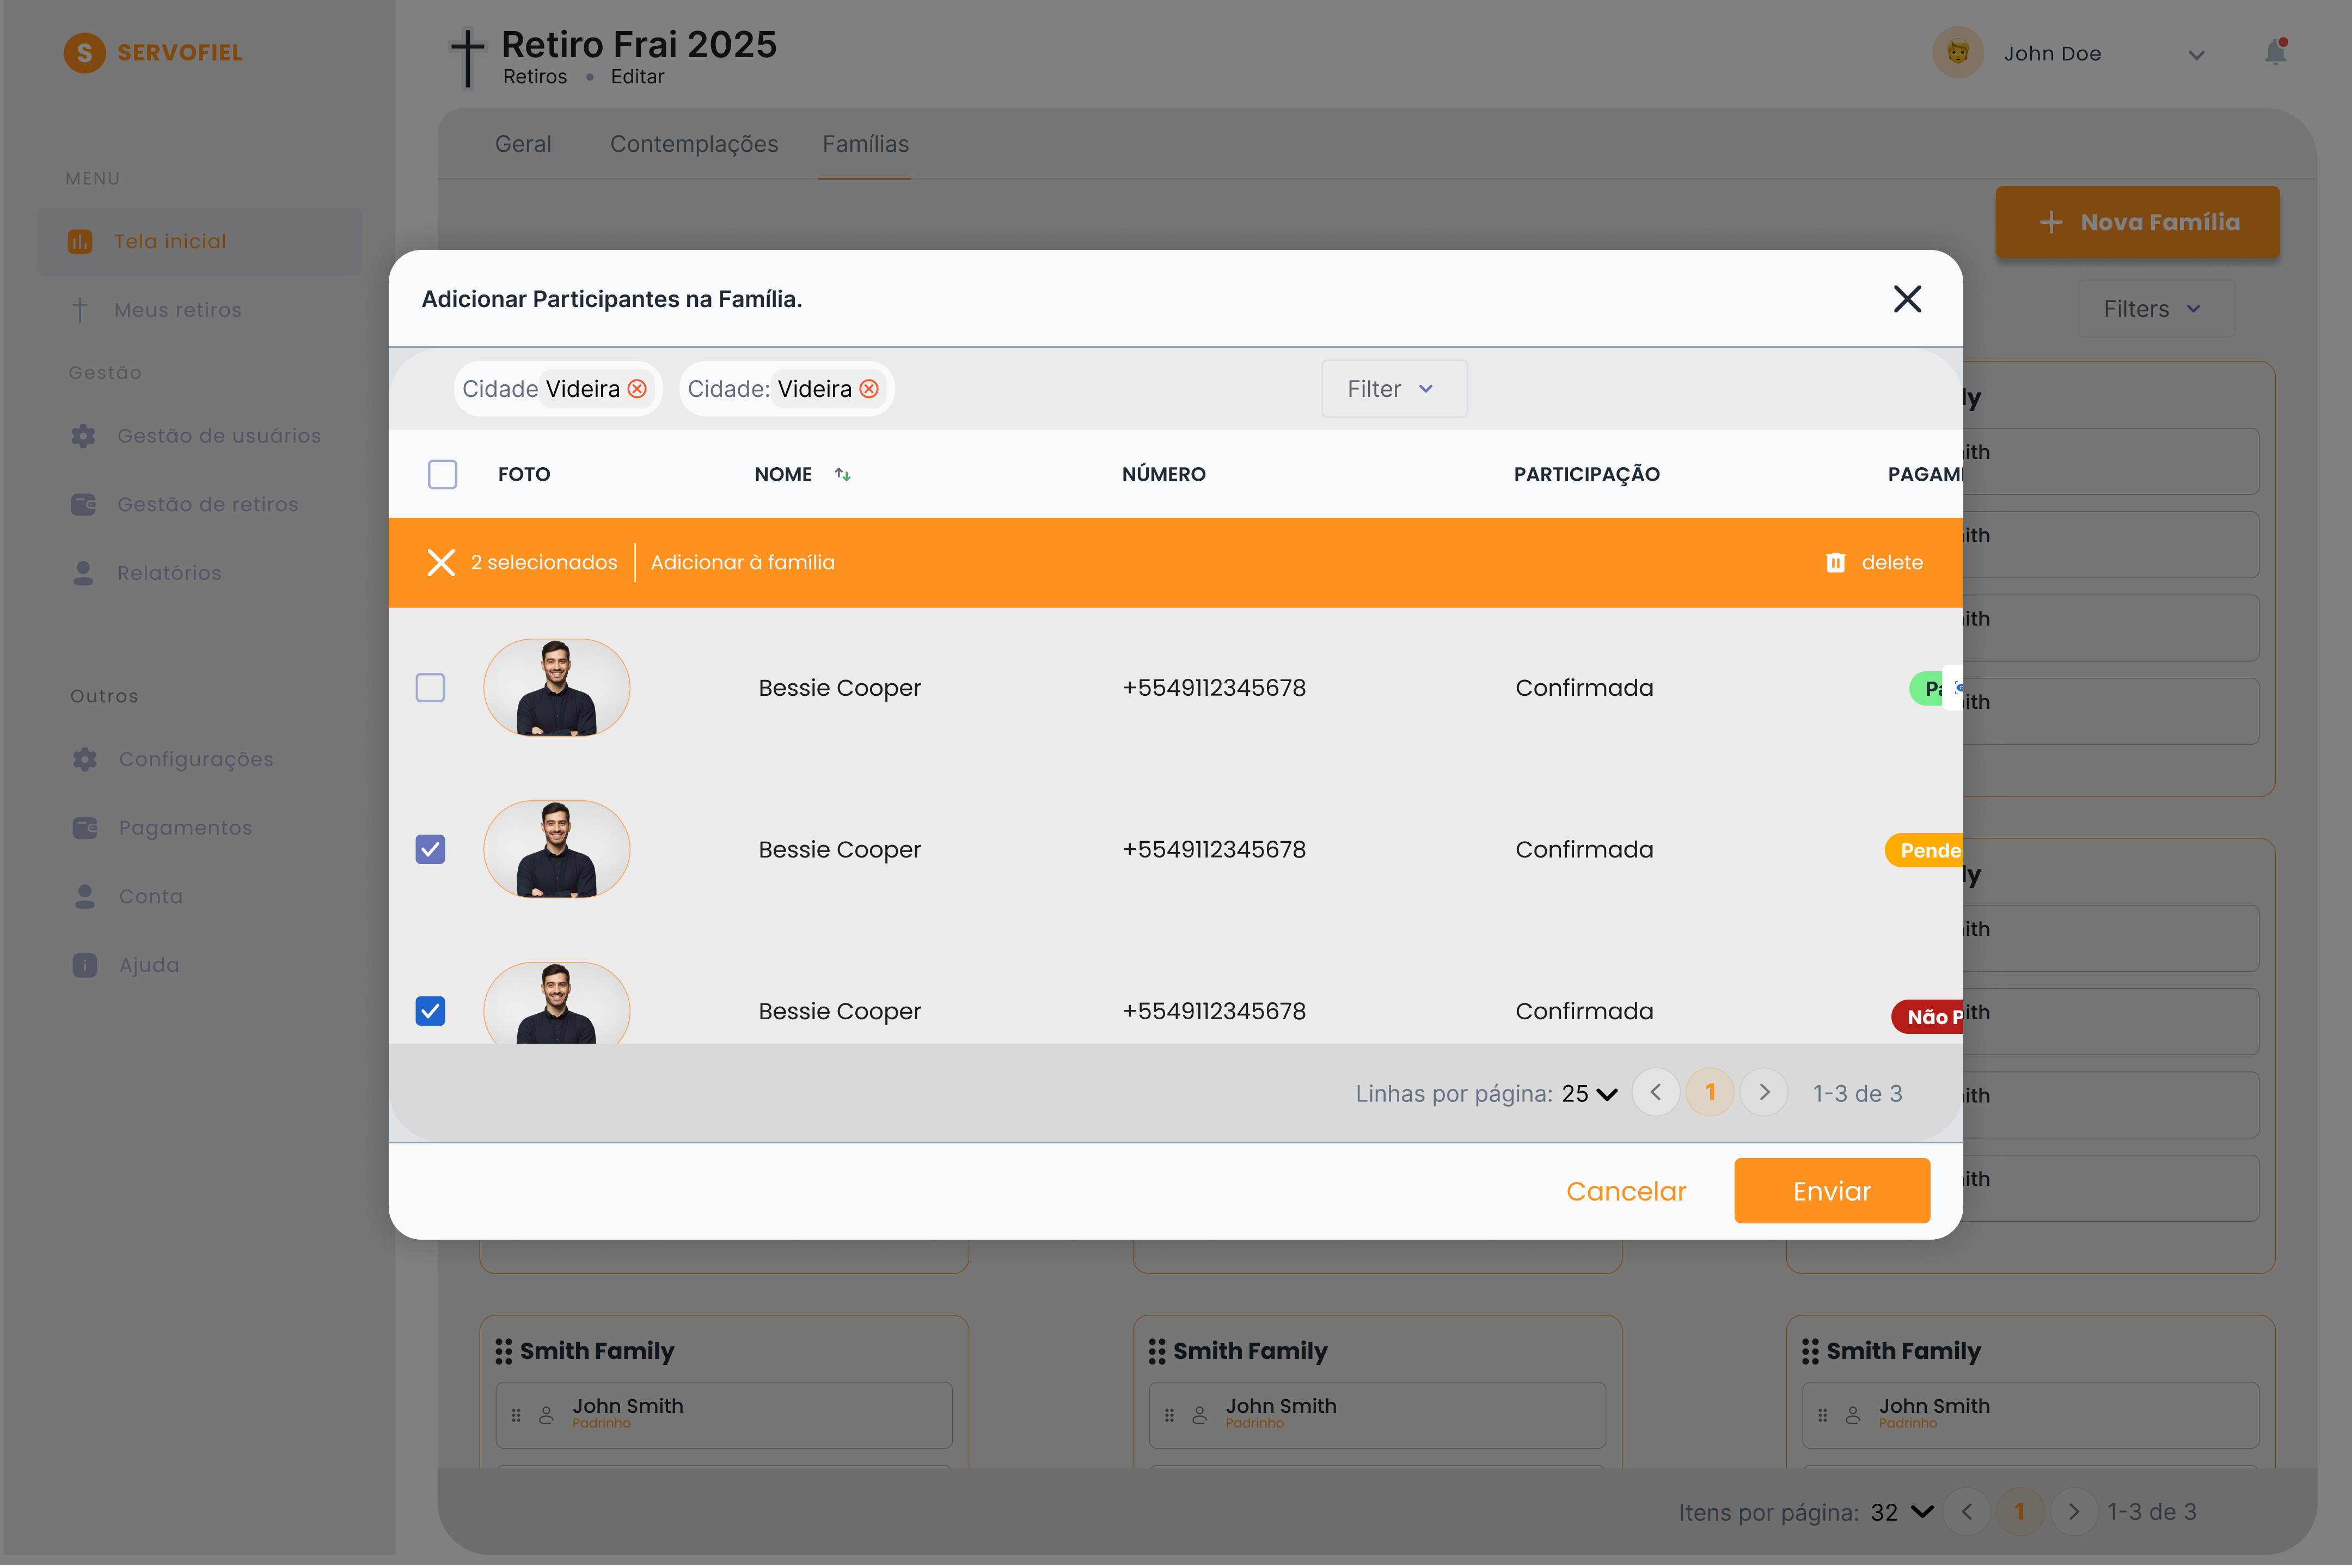
\includegraphics[width=0.8\textwidth]{images/prototipacao/familia/Familias.png}
\caption{Adição de múltiplos participantes na família.}
\end{figure}

\begin{figure}[H]
\centering
\includegraphics[width=0.8\textwidth]{images/prototipacao/barracaEequipeDeServico/Equipes de serviço.png}
\caption{Tela inicial das equipes de serviço.}
\end{figure}

\begin{figure}[H]
\centering
\includegraphics[width=0.8\textwidth]{images/prototipacao/barracaEequipeDeServico/Gestão de Barracas.png}
\caption{Tela inicial das barracas.}
\end{figure}

\begin{figure}[H]
\centering
\includegraphics[width=0.8\textwidth]{images/prototipacao/relatorios/Relatórios-1.png}
\caption{Tela inicial dos relatórios.}
\end{figure}

\begin{figure}[H]
\centering
\includegraphics[width=0.8\textwidth]{images/prototipacao/relatorios/Relatórios.png}
\caption{Formulário para edição ou criação dos relatórios.}
\end{figure}

\begin{figure}[H]
\centering
\includegraphics[width=0.8\textwidth]{images/prototipacao/relatorios/Gestão de Usuarios.png}
\caption{Resultado dos filtros.}
\end{figure}

\begin{figure}[H]
\centering
\includegraphics[width=0.8\textwidth]{images/prototipacao/relatorios/Gestão de Usuarios-1.png}
\caption{Configuração dos filtros.}
\end{figure}

\begin{figure}[H]
\centering
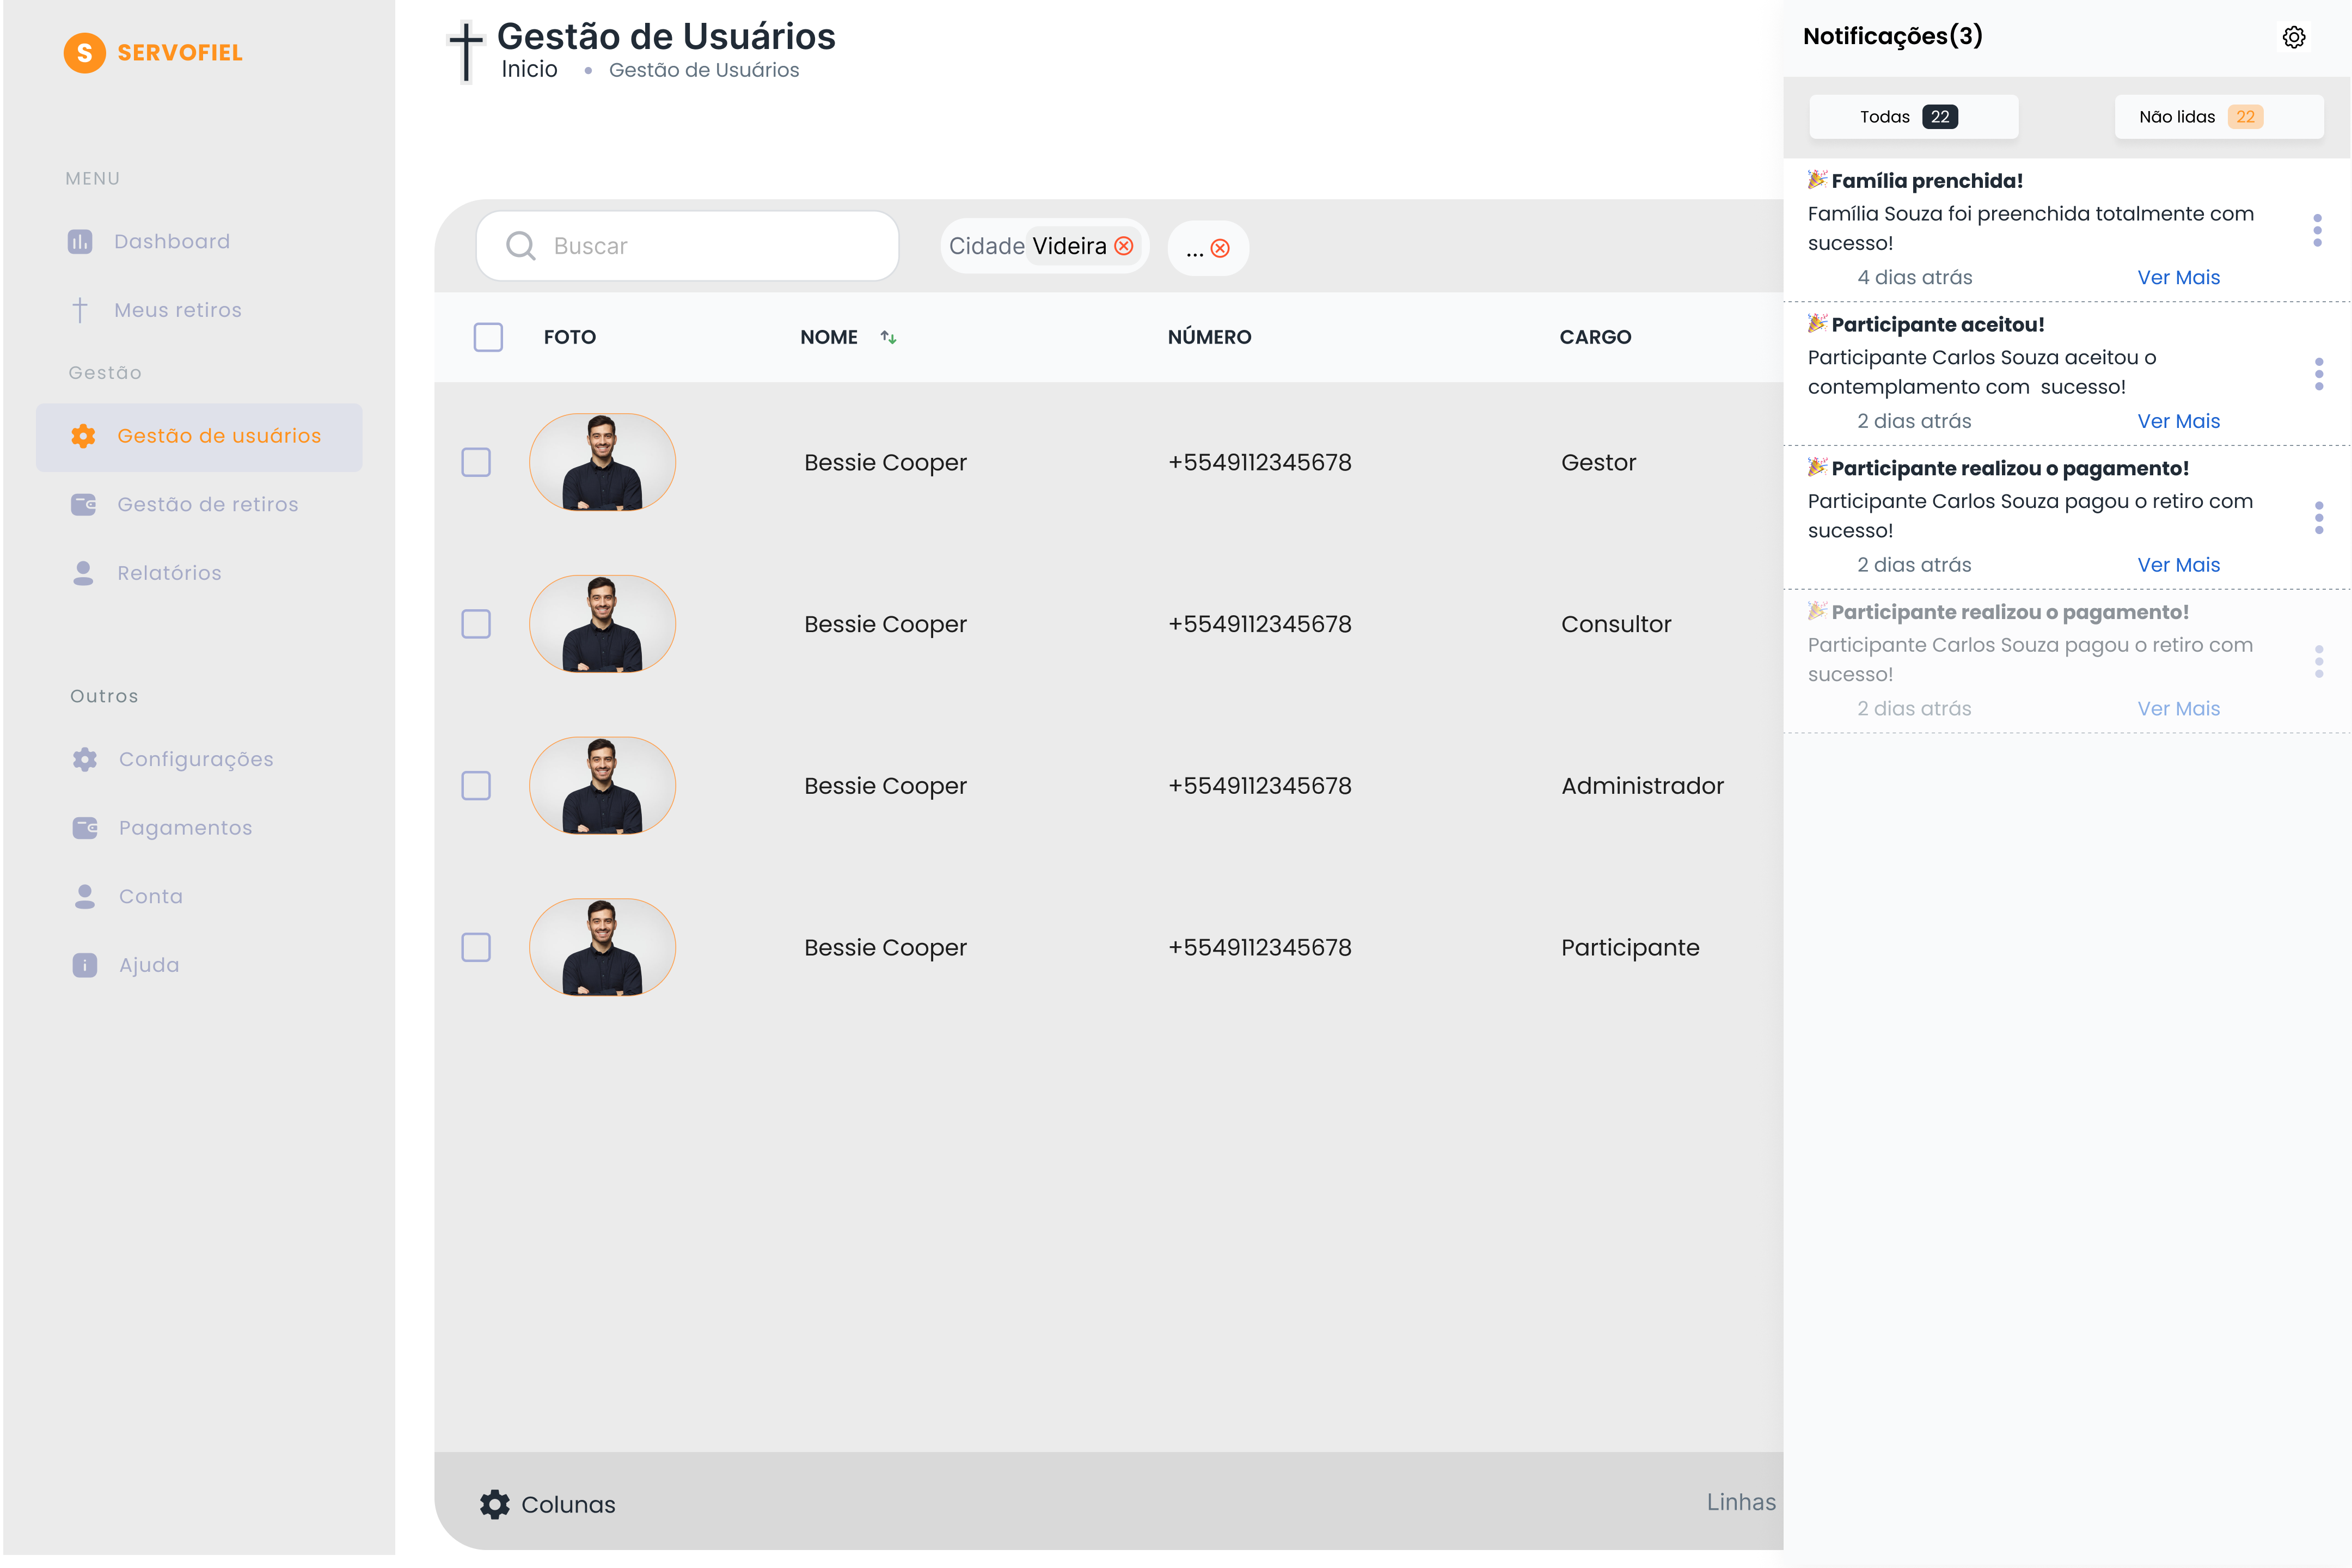
\includegraphics[width=0.8\textwidth]{images/prototipacao/notificacoes/Notificações.png}
\caption{Painel lateral de notificações do sistema. Exibe alertas e mensagens relevantes ao usuário, incluindo atualizações sobre inscrições, contemplações, pagamentos e outras ações realizadas no sistema.}
\end{figure}

\begin{figure}[H]
\centering
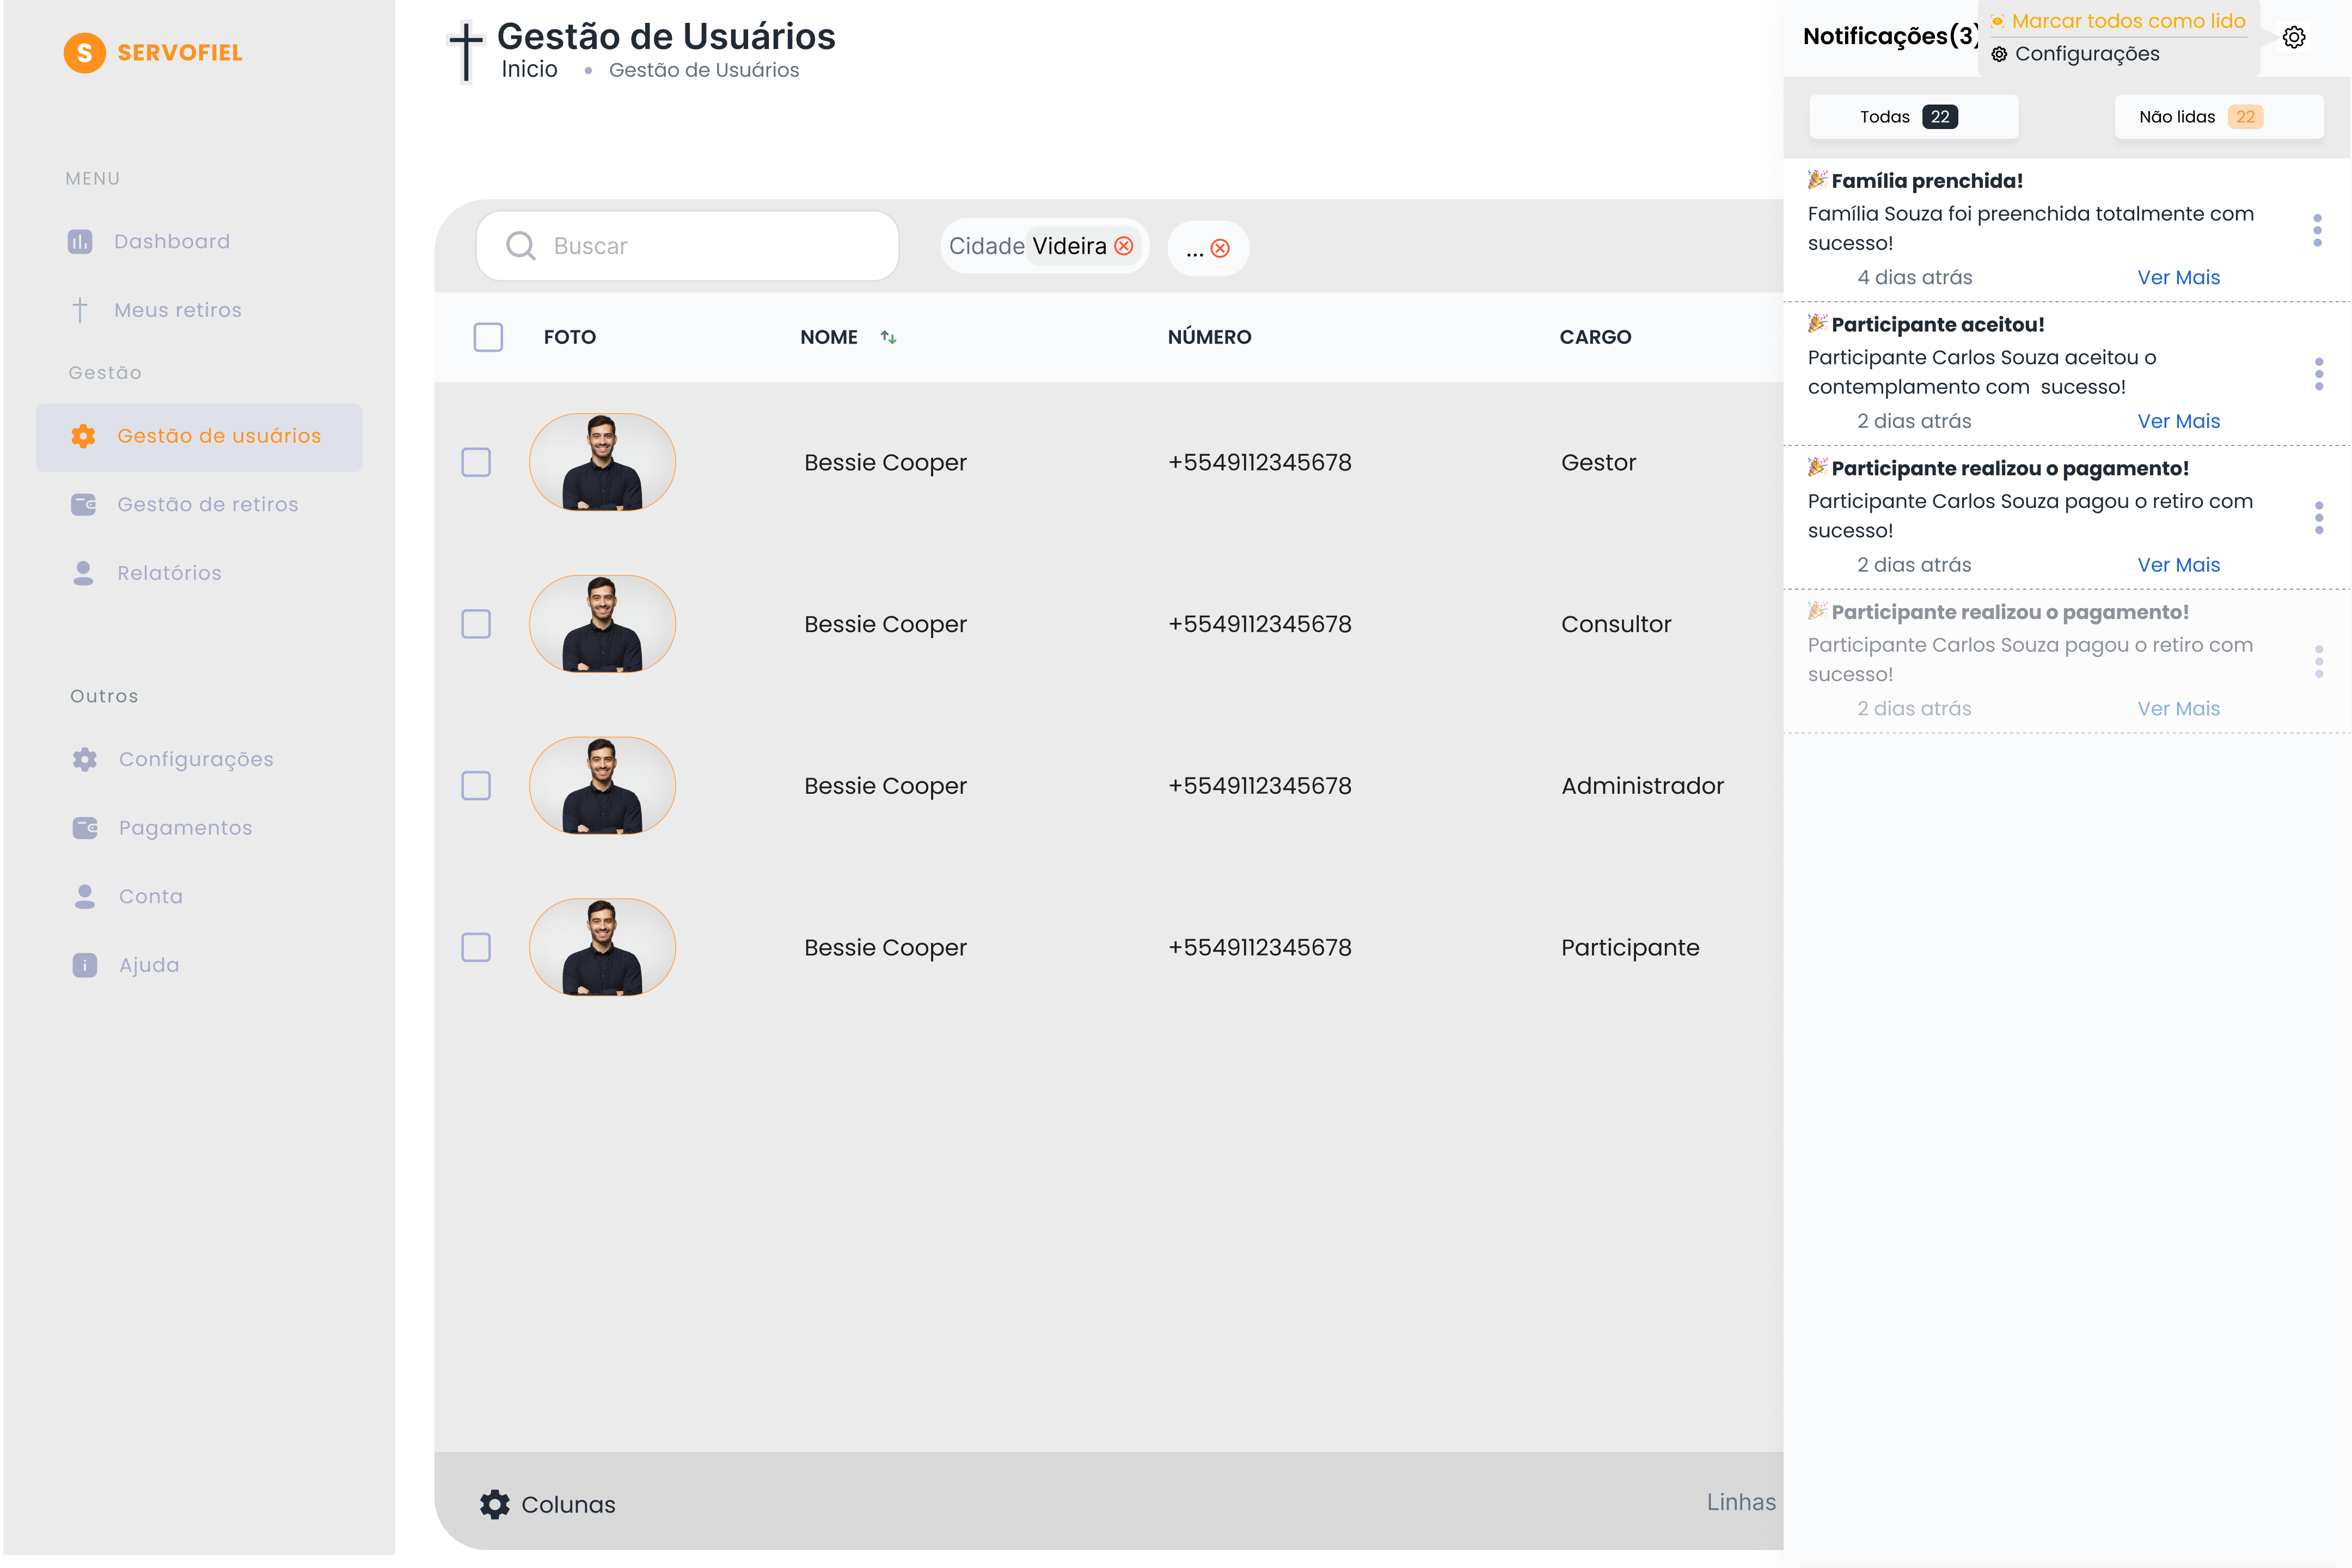
\includegraphics[width=0.8\textwidth]{images/prototipacao/notificacoes/Notificações-1.png}
\caption{Popover  com botões para acessar as configurações das notificações.}
\end{figure}

\begin{figure}[H]
\centering
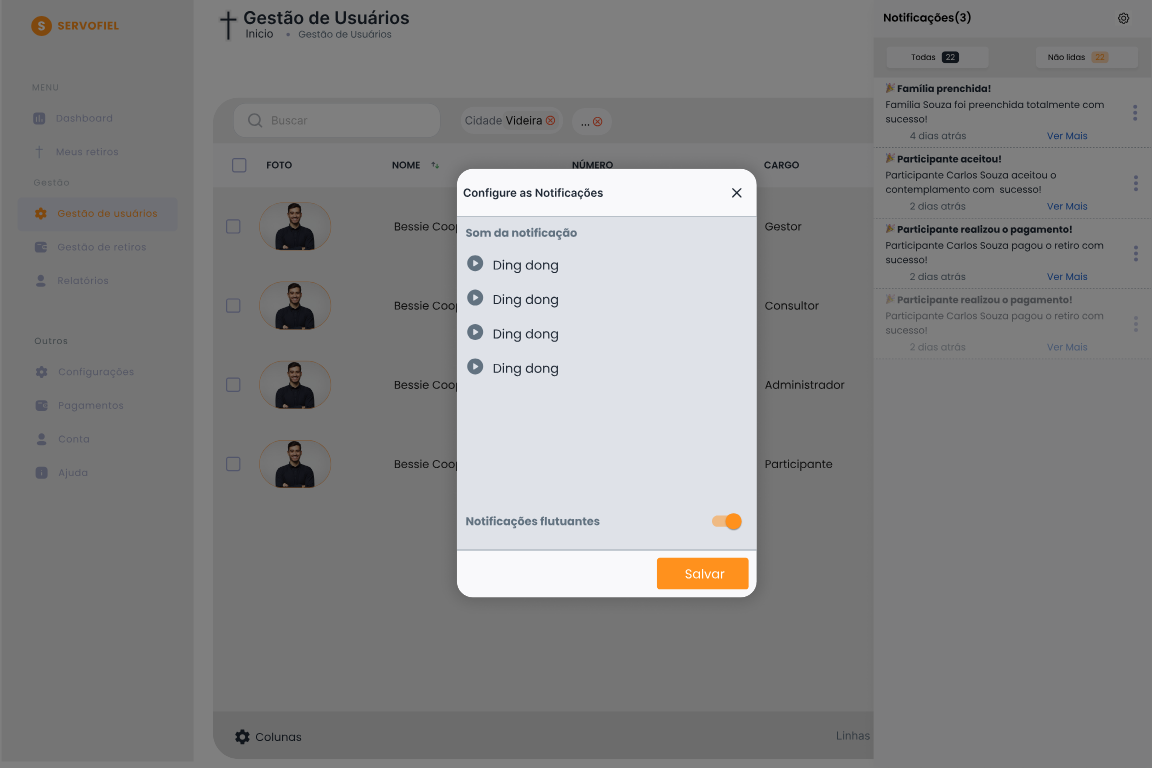
\includegraphics[width=0.8\textwidth]{images/prototipacao/notificacoes/notificacoesmodal.png}
\caption{Modal com as configurações das notificaões.}
\end{figure}


Esses protótipos possibilitaram validar a experiência do usuário em diferentes perfis de acesso (Administrador, Gestor e Consultor), além de antecipar ajustes visuais e comportamentais antes da implementação do sistema. Os fluxos de navegação detalhados estão documentados por meio de diagramas de sequência no capítulo correspondente.
O protótipo completo da interface, com todos os fluxos interativos detalhados, está disponível no \textbf{Anexo A}.f
\section{Diagramas de Sequência}

Nesta seção, são apresentados os diagramas de sequência que descrevem o comportamento dinâmico do sistema frente às interações dos usuários com as principais funcionalidades.

\subsection{Diagrama de Sequência – Criação de Novo Usuário}

A Figura~\ref{fig:diagrama-criacao-usuario} ilustra o fluxo realizado pelo administrador ao criar um novo usuário no sistema. Esse processo envolve o acesso ao módulo de gestão de usuários, abertura do formulário de cadastro, preenchimento dos campos necessários, validação dos dados e envio para o backend.

\begin{figure}[H]
    \centering
    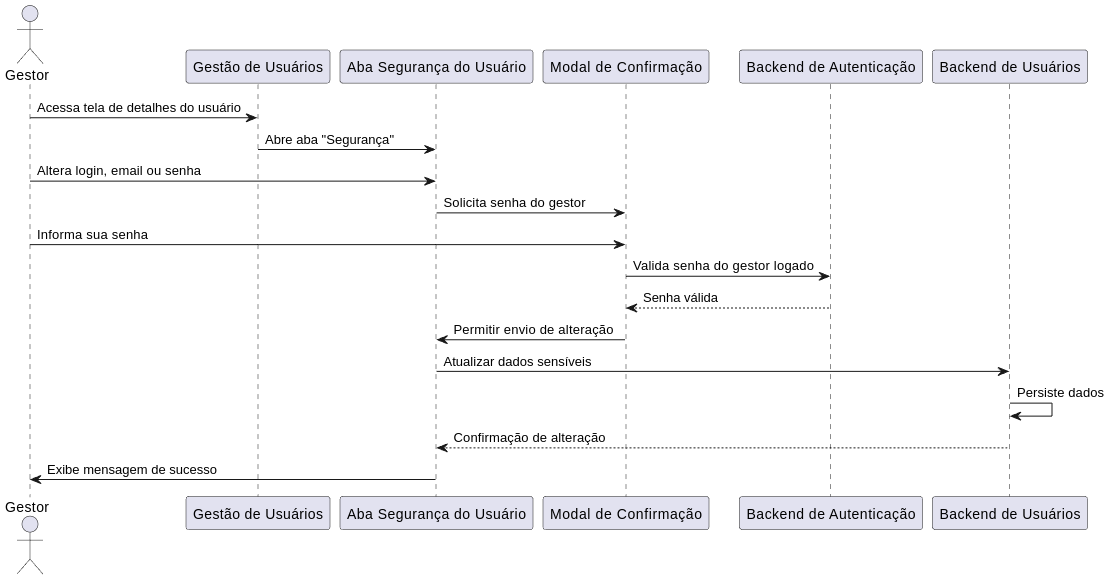
\includegraphics[width=0.9\textwidth]{images/diagramasdesequencias/usercreate.png}
    \caption{Diagrama de sequência para criação de novo usuário}
    \label{fig:diagrama-criacao-usuario}
\end{figure}

O fluxo se inicia quando o administrador clica no botão “+ Novo Usuário”. O sistema exibe o formulário de cadastro, onde o administrador preenche os dados como nome, e-mail, senha e papel do usuário. O formulário aciona a validação dos campos obrigatórios. Com os dados validados, a informação é enviada ao backend, que cria o novo registro no banco de dados. Em seguida, o sistema exibe uma mensagem de sucesso e atualiza a lista de usuários visível para o administrador.

\subsection{Diagrama de Sequência – Visualização e Edição de Permissões}

A Figura~\ref{fig:diagrama-permissoes} ilustra o fluxo realizado pelo administrador para visualizar e editar as permissões de um usuário. O processo envolve a seleção do usuário, acesso à aba de permissões e modificação das permissões conforme necessário.

\begin{figure}[H]
    \centering
    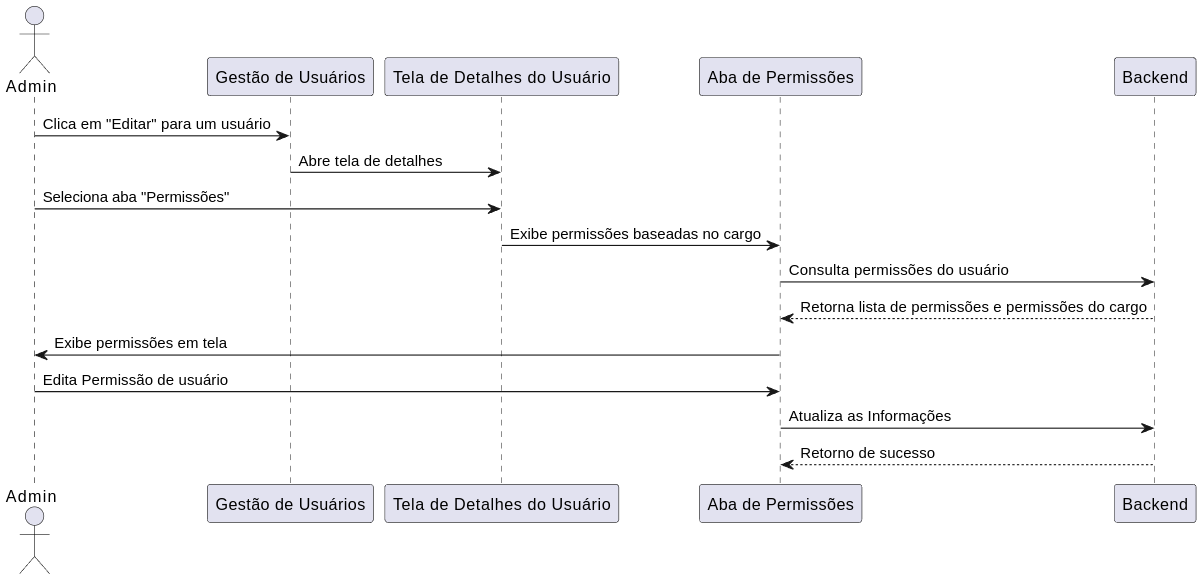
\includegraphics[width=0.9\textwidth]{images/diagramasdesequencias/userEditPermissions.png}
    \caption{Diagrama de sequência para visualização e edição de permissões de usuário}
    \label{fig:diagrama-permissoes}
\end{figure}

\subsection{Diagrama de Sequência – Edição de Informações do Usuário}

A Figura~\ref{fig:diagrama-edicao-usuario} ilustra o fluxo realizado pelo administrador ao editar informações cadastrais de um usuário. Esse processo permite a atualização de dados como nome, cidade, data de nascimento e cargo.

\begin{figure}[H]
    \centering
    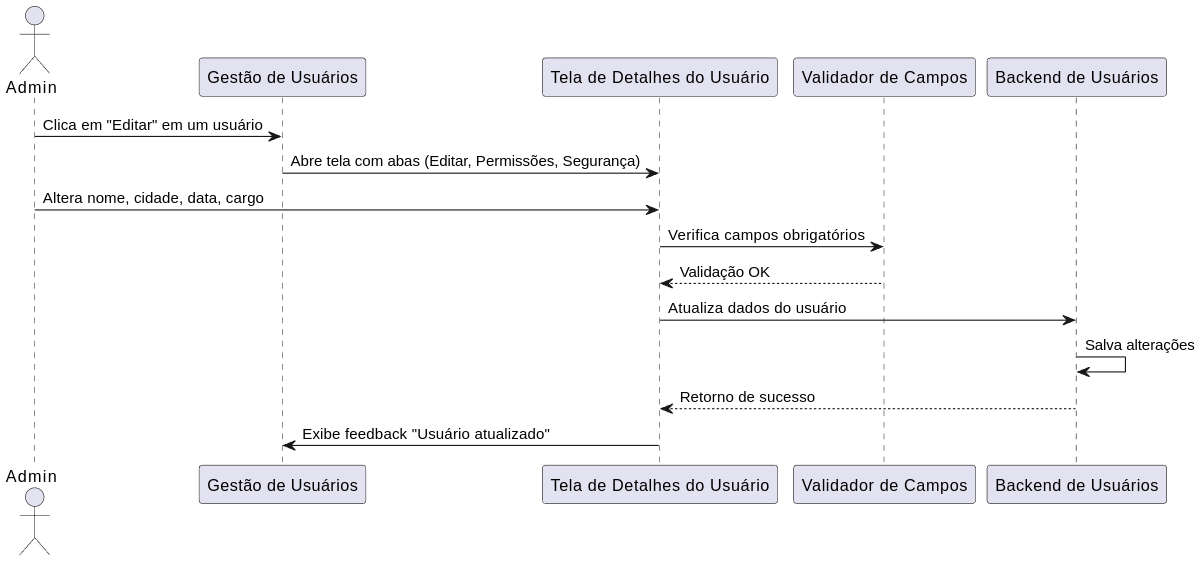
\includegraphics[width=0.9\textwidth]{images/diagramasdesequencias/userEdit.png}
    \caption{Diagrama de sequência para edição de informações do usuário}
    \label{fig:diagrama-edicao-usuario}
\end{figure}

O fluxo se inicia quando o administrador acessa o módulo de gestão de usuários e clica na opção “Editar” para um usuário específico. A tela de detalhes do usuário é carregada com múltiplas abas, sendo selecionada a aba de edição. Após realizar as alterações nos campos, o sistema valida os dados obrigatórios. Com a validação concluída, os dados são enviados ao backend para atualização no banco de dados. Por fim, uma mensagem de sucesso é exibida ao administrador confirmando a atualização.

\subsection{Diagrama de Sequência – Edição de Dados Sensíveis com Confirmação}

A Figura~\ref{fig:diagrama-dados-sensiveis} apresenta o fluxo que ocorre quando o gestor edita dados sensíveis de um usuário, como login, e-mail ou senha. Este processo exige uma etapa adicional de autenticação para garantir a segurança da operação.

\begin{figure}[H]
    \centering
    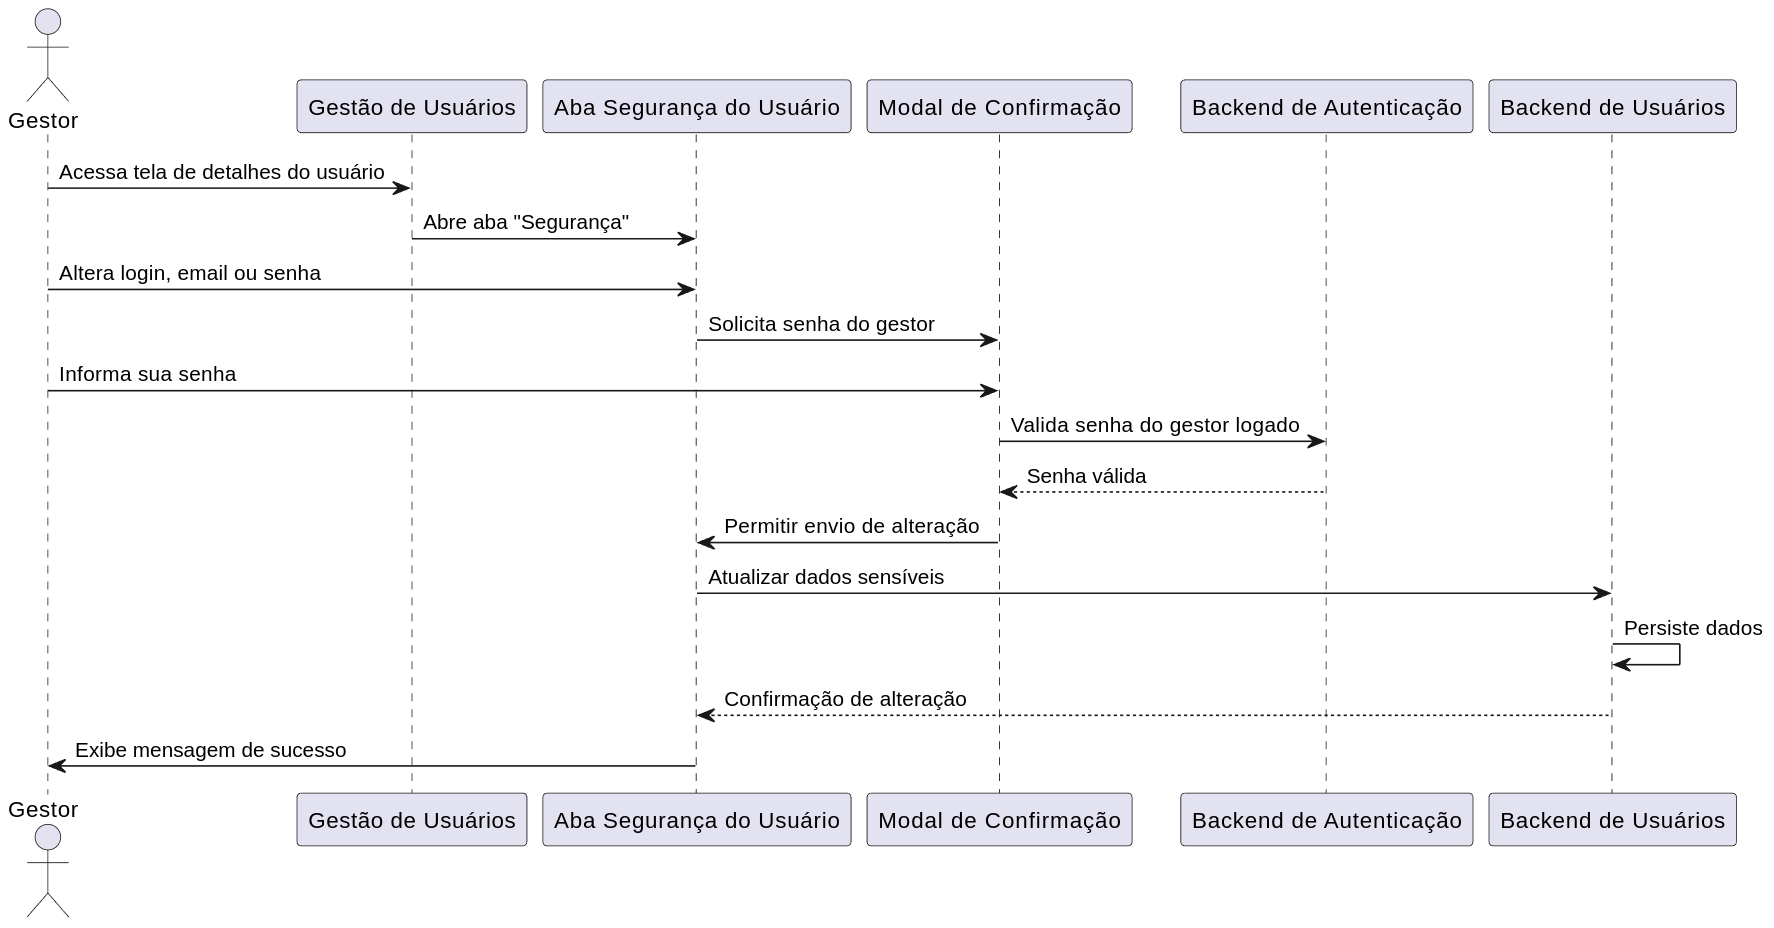
\includegraphics[width=0.9\textwidth]{images/diagramasdesequencias/userCredentials.png}
    \caption{Diagrama de sequência para edição de dados sensíveis com confirmação}
    \label{fig:diagrama-dados-sensiveis}
\end{figure}

O fluxo inicia-se com o gestor acessando a tela de detalhes do usuário e navegando até a aba “Segurança”. Ao tentar alterar dados sensíveis, como login, e-mail ou senha, o sistema exibe um modal solicitando a senha do gestor para confirmar a ação. Após a senha ser informada, ela é validada pelo backend de autenticação. Com a validação bem-sucedida, o sistema autoriza a atualização, que é enviada ao backend de usuários. Após a persistência dos dados no banco, o sistema exibe uma mensagem de confirmação ao gestor.

\subsection{Diagrama de Sequência – Login de Usuário}

A Figura~\ref{fig:normalLogin} apresenta o fluxo completo do processo de autenticação de um usuário no sistema. Esse processo envolve a verificação das credenciais, a inicialização da sessão e a exibição da interface conforme o papel atribuído ao usuário.

\begin{figure}[H]
    \centering
    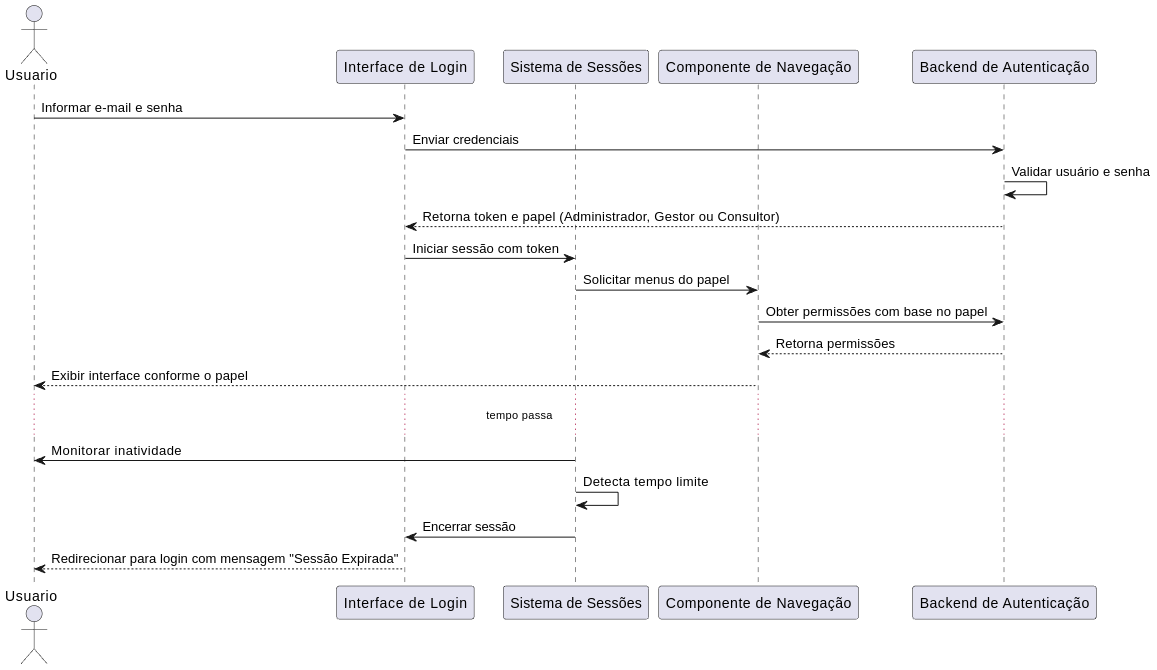
\includegraphics[width=0.9\textwidth]{images/diagramasdesequencias/normalLogin.png}
    \caption{Diagrama de sequência para login de usuário}
    \label{fig:normalLogin}
\end{figure}

O fluxo inicia-se quando o usuário informa seu e-mail e senha na interface de login. As credenciais são enviadas ao backend de autenticação, que realiza a validação e retorna um token e o papel do usuário (Administrador, Gestor ou Consultor). A sessão é iniciada com base nesse token, e a interface de navegação solicita ao backend as permissões correspondentes ao papel. Com base nas permissões, a interface adaptada é exibida ao usuário.

Após o login, o sistema monitora a atividade do usuário. Caso ocorra inatividade por tempo prolongado, a sessão é finalizada automaticamente, redirecionando o usuário à tela de login com a mensagem "Sessão Expirada".

\subsection{Diagrama de Sequência – Cadastro de Retiro}

A Figura~\ref{fig:retreatCreate} apresenta o fluxo realizado pelo gestor ao cadastrar um novo retiro no sistema. Esse processo envolve a abertura do formulário, preenchimento das informações principais, validação dos campos obrigatórios e comunicação com o backend para persistência dos dados.

\begin{figure}[H]
    \centering
    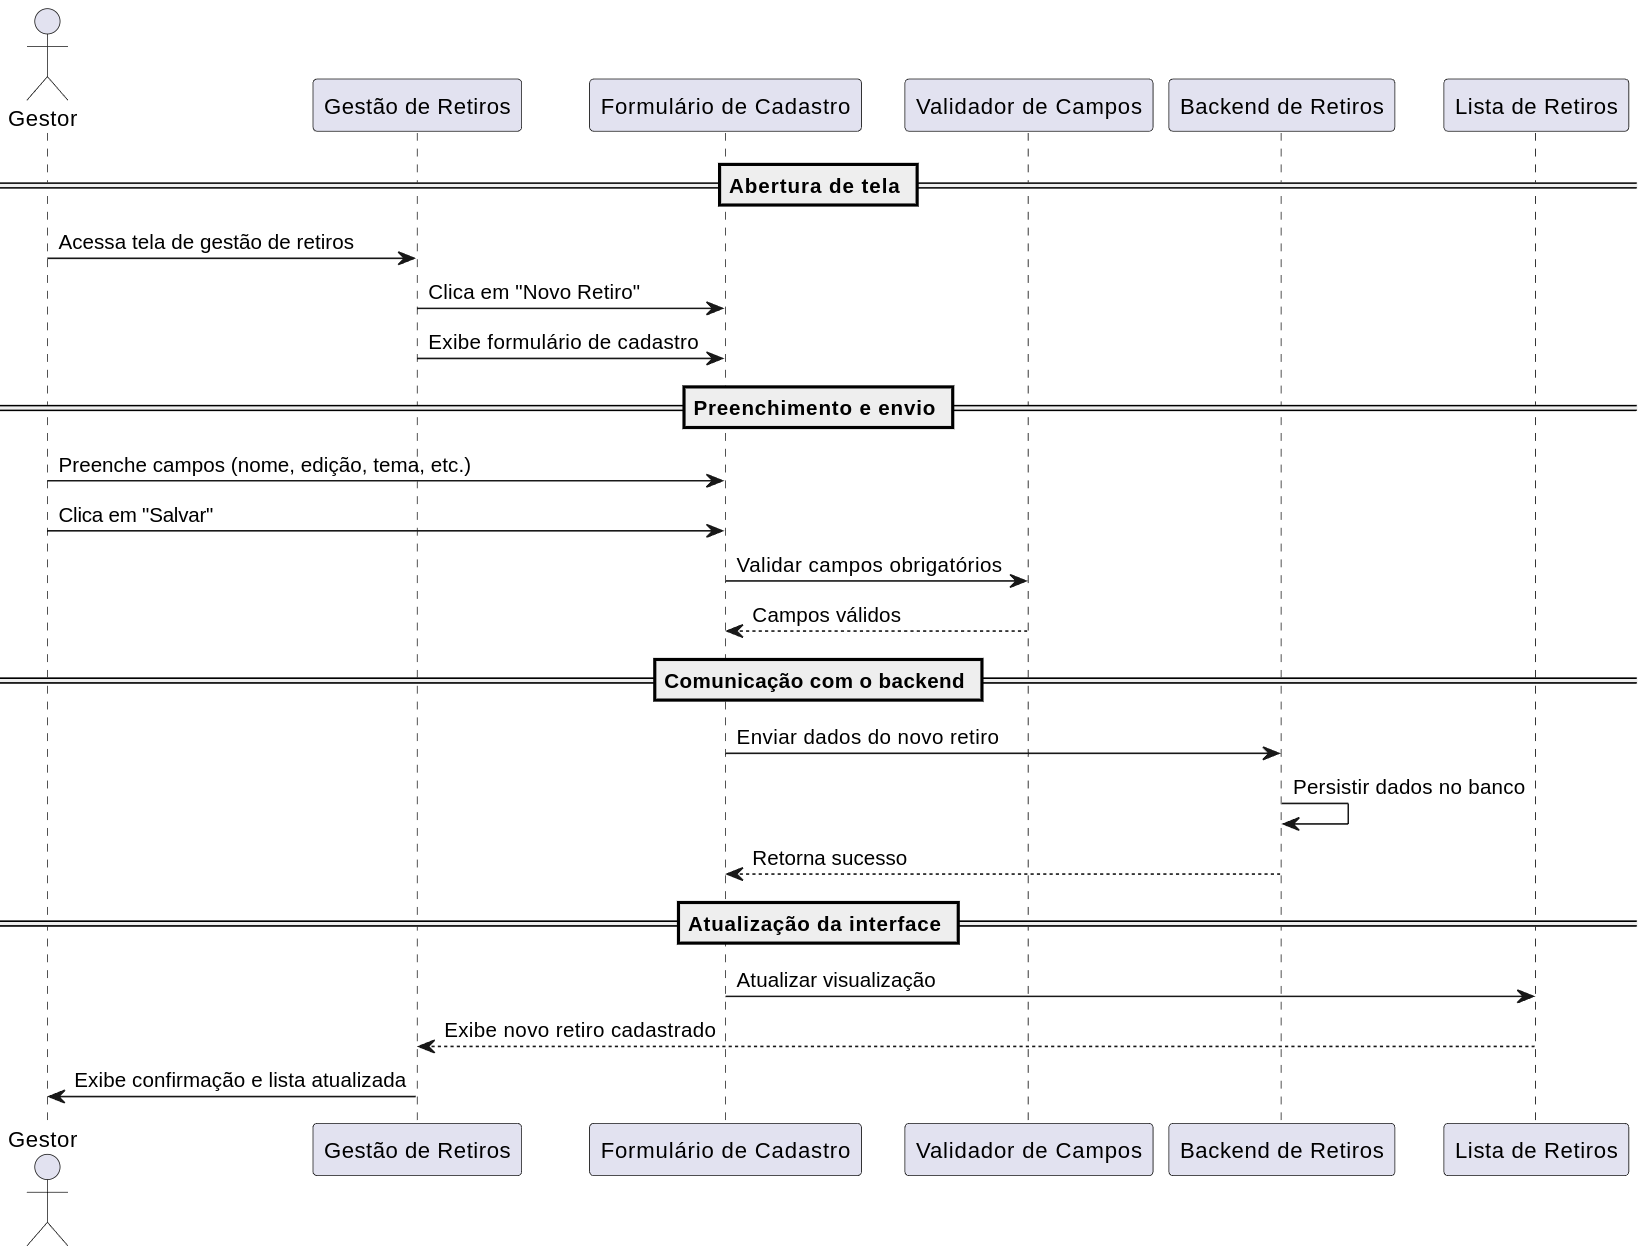
\includegraphics[width=0.9\textwidth]{images/diagramasdesequencias/retreatCreate.png}
    \caption{Diagrama de sequência para cadastro de retiro}
    \label{fig:retreatCreate}
\end{figure}

Inicialmente, o gestor acessa a tela de gestão de retiros e clica na opção “Novo Retiro”, o que aciona a exibição do formulário de cadastro. Após preencher os campos como nome, edição e tema, o gestor clica em “Salvar”. Os dados são validados e, se estiverem corretos, enviados ao backend para persistência. Ao final do processo, a lista de retiros é atualizada e o sistema exibe uma confirmação do cadastro.

\subsection{Diagrama de Sequência – Inativação de Retiro}

A Figura~\ref{fig:retreatInativation} apresenta o fluxo realizado pelo gestor para inativar um retiro previamente cadastrado. O processo envolve a seleção do retiro, confirmação da ação e atualização do status na interface.

\begin{figure}[H]
    \centering
    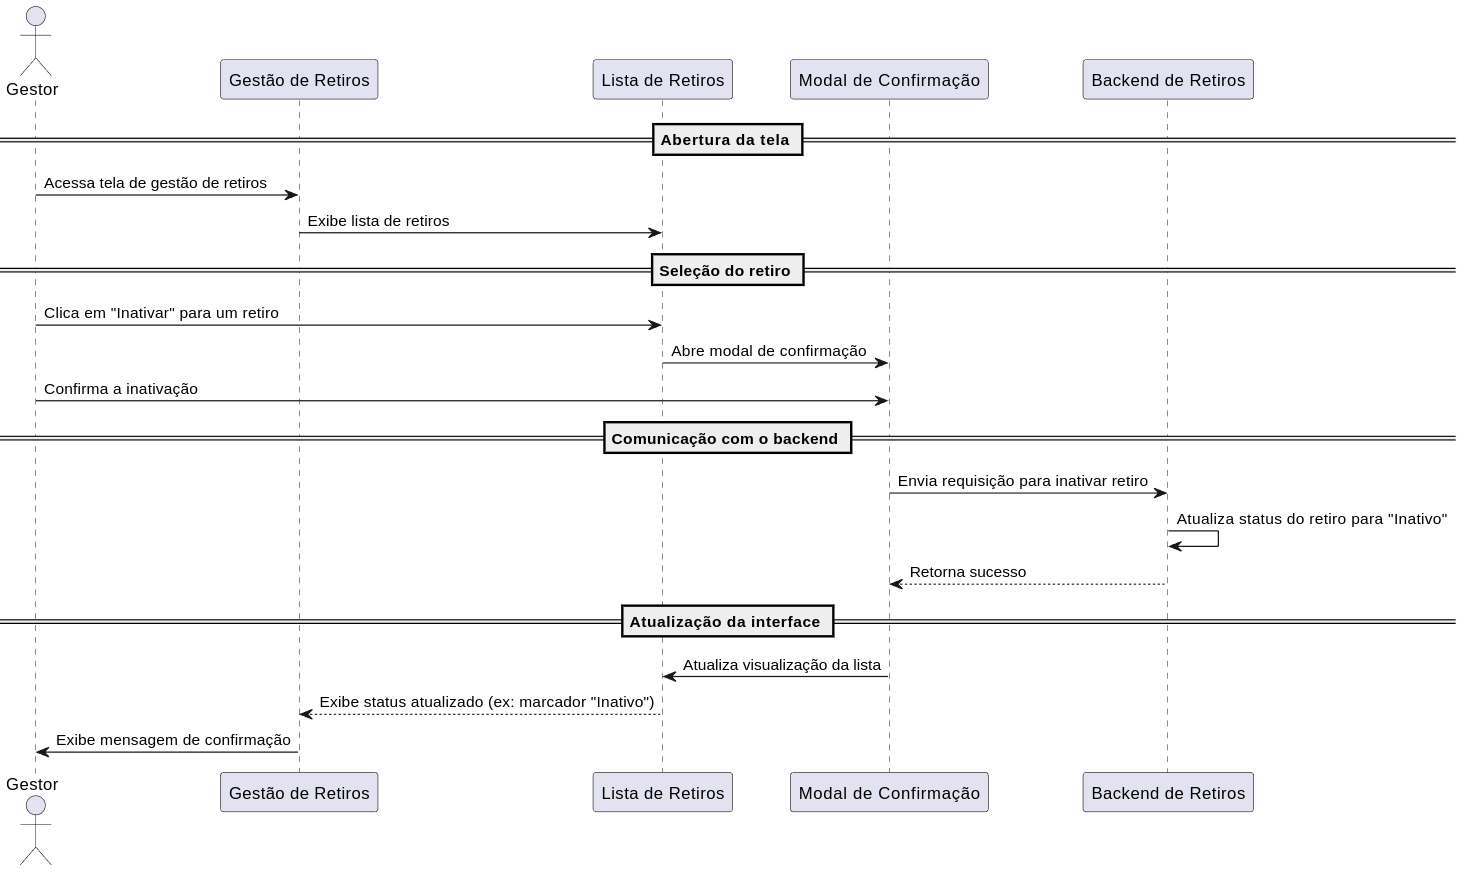
\includegraphics[width=0.9\textwidth]{images/diagramasdesequencias/retreatInativation.png}
    \caption{Diagrama de sequência para inativação de retiro}
    \label{fig:retreatInativation}
\end{figure}

O fluxo inicia com o gestor acessando a tela de gestão de retiros, onde é exibida a lista de eventos. Ao clicar em “Inativar” para um retiro específico, um modal de confirmação é apresentado. Após a confirmação, a requisição é enviada ao backend, que atualiza o status do retiro para “Inativo”. O sistema então retorna uma confirmação, atualiza a interface com um marcador indicativo e exibe uma mensagem de sucesso ao gestor.

\subsection{Diagrama de Sequência – Gerador de Formulário Personalizado}

A Figura~\ref{fig:retreatFormCreate} apresenta o fluxo realizado pelo gestor ao acessar e personalizar os formulários vinculados a um retiro. O sistema permite criar e editar formulários específicos tanto para os participantes quanto para as equipes de serviço, de forma modular.

\begin{figure}[H]
    \centering
    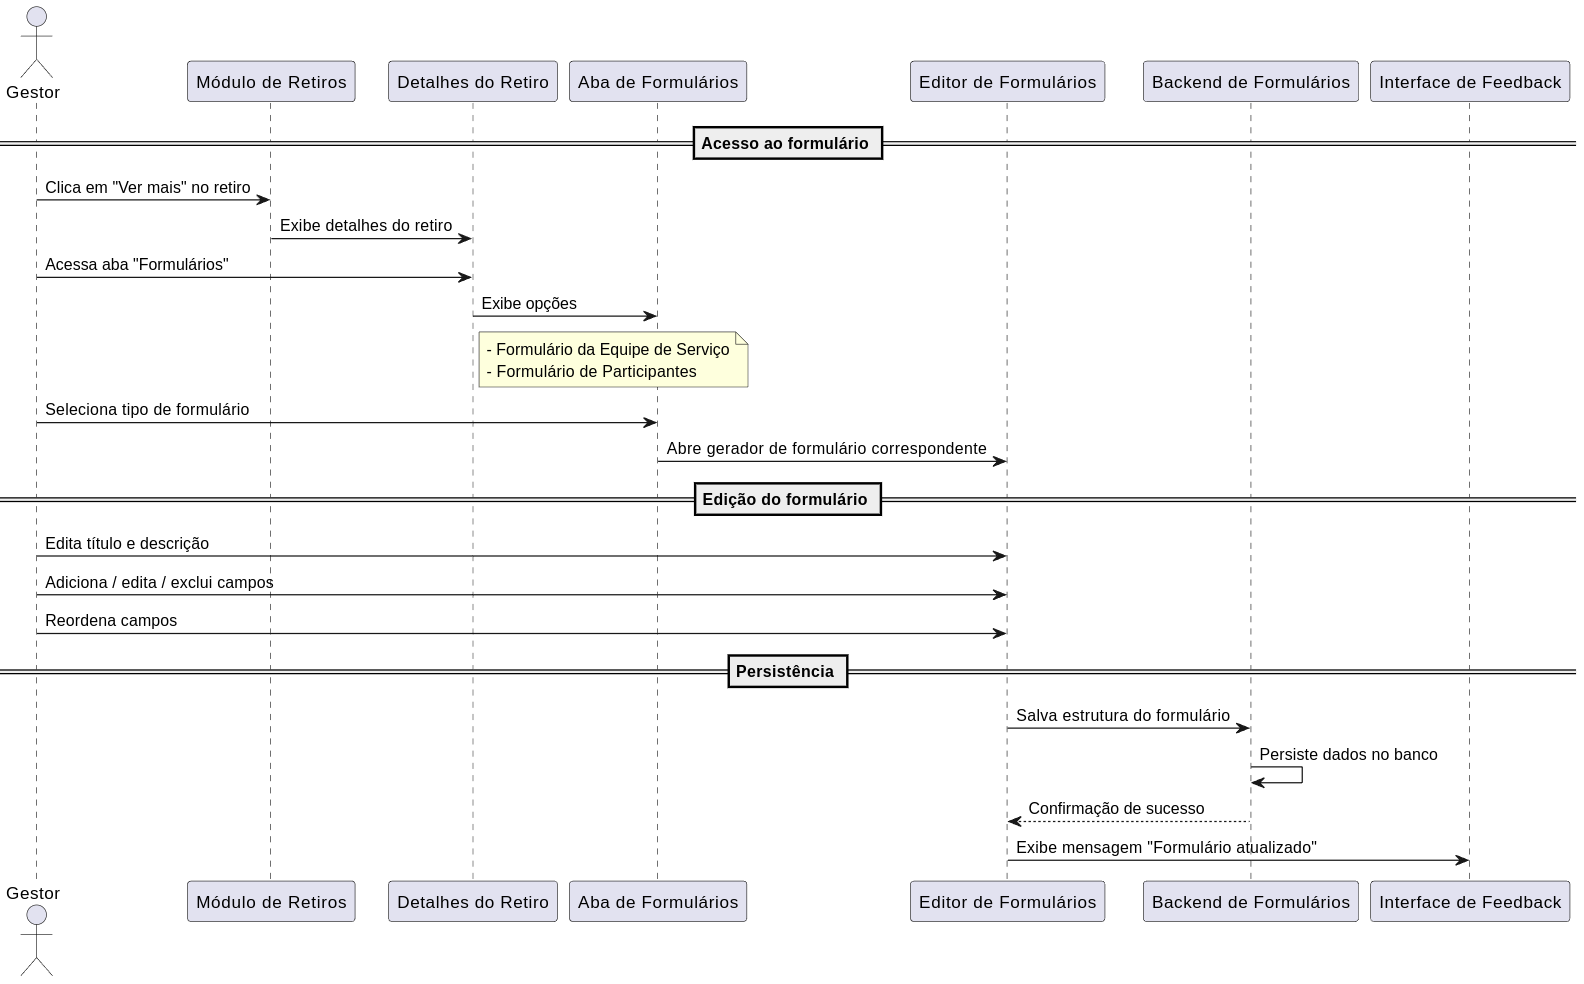
\includegraphics[width=0.9\textwidth]{images/diagramasdesequencias/retreatFormCreate.png}
    \caption{Diagrama de sequência para criação de formulário personalizado para um retiro}
    \label{fig:retreatFormCreate}
\end{figure}

O processo tem início quando o gestor acessa a área de detalhes de um retiro e seleciona a aba “Formulários”. Nessa aba, é possível escolher entre diferentes tipos de formulário. Como cada retiro tem 2 formulários(Participantes e equipe de serviço), você decide para qual grupo você irá editar, ao selecionar um deles, o sistema abre o editor correspondente. No editor, o gestor pode modificar o título, a descrição, adicionar ou remover campos e reordená-los conforme necessário. Ao salvar, o editor envia os dados ao backend, que persiste a estrutura do formulário e retorna uma confirmação. Por fim, uma mensagem é exibida ao gestor informando que a atualização foi bem-sucedida.

\subsection{Diagrama de Sequência – Inscrição Manual via Sistema}

A Figura~\ref{fig:manualParticipantInscription} descreve o fluxo completo para realização de inscrições manuais pelo gestor dentro do sistema, contemplando tanto o cadastro individual quanto a importação em lote via arquivo `.csv`.

\begin{figure}[H]
    \centering
    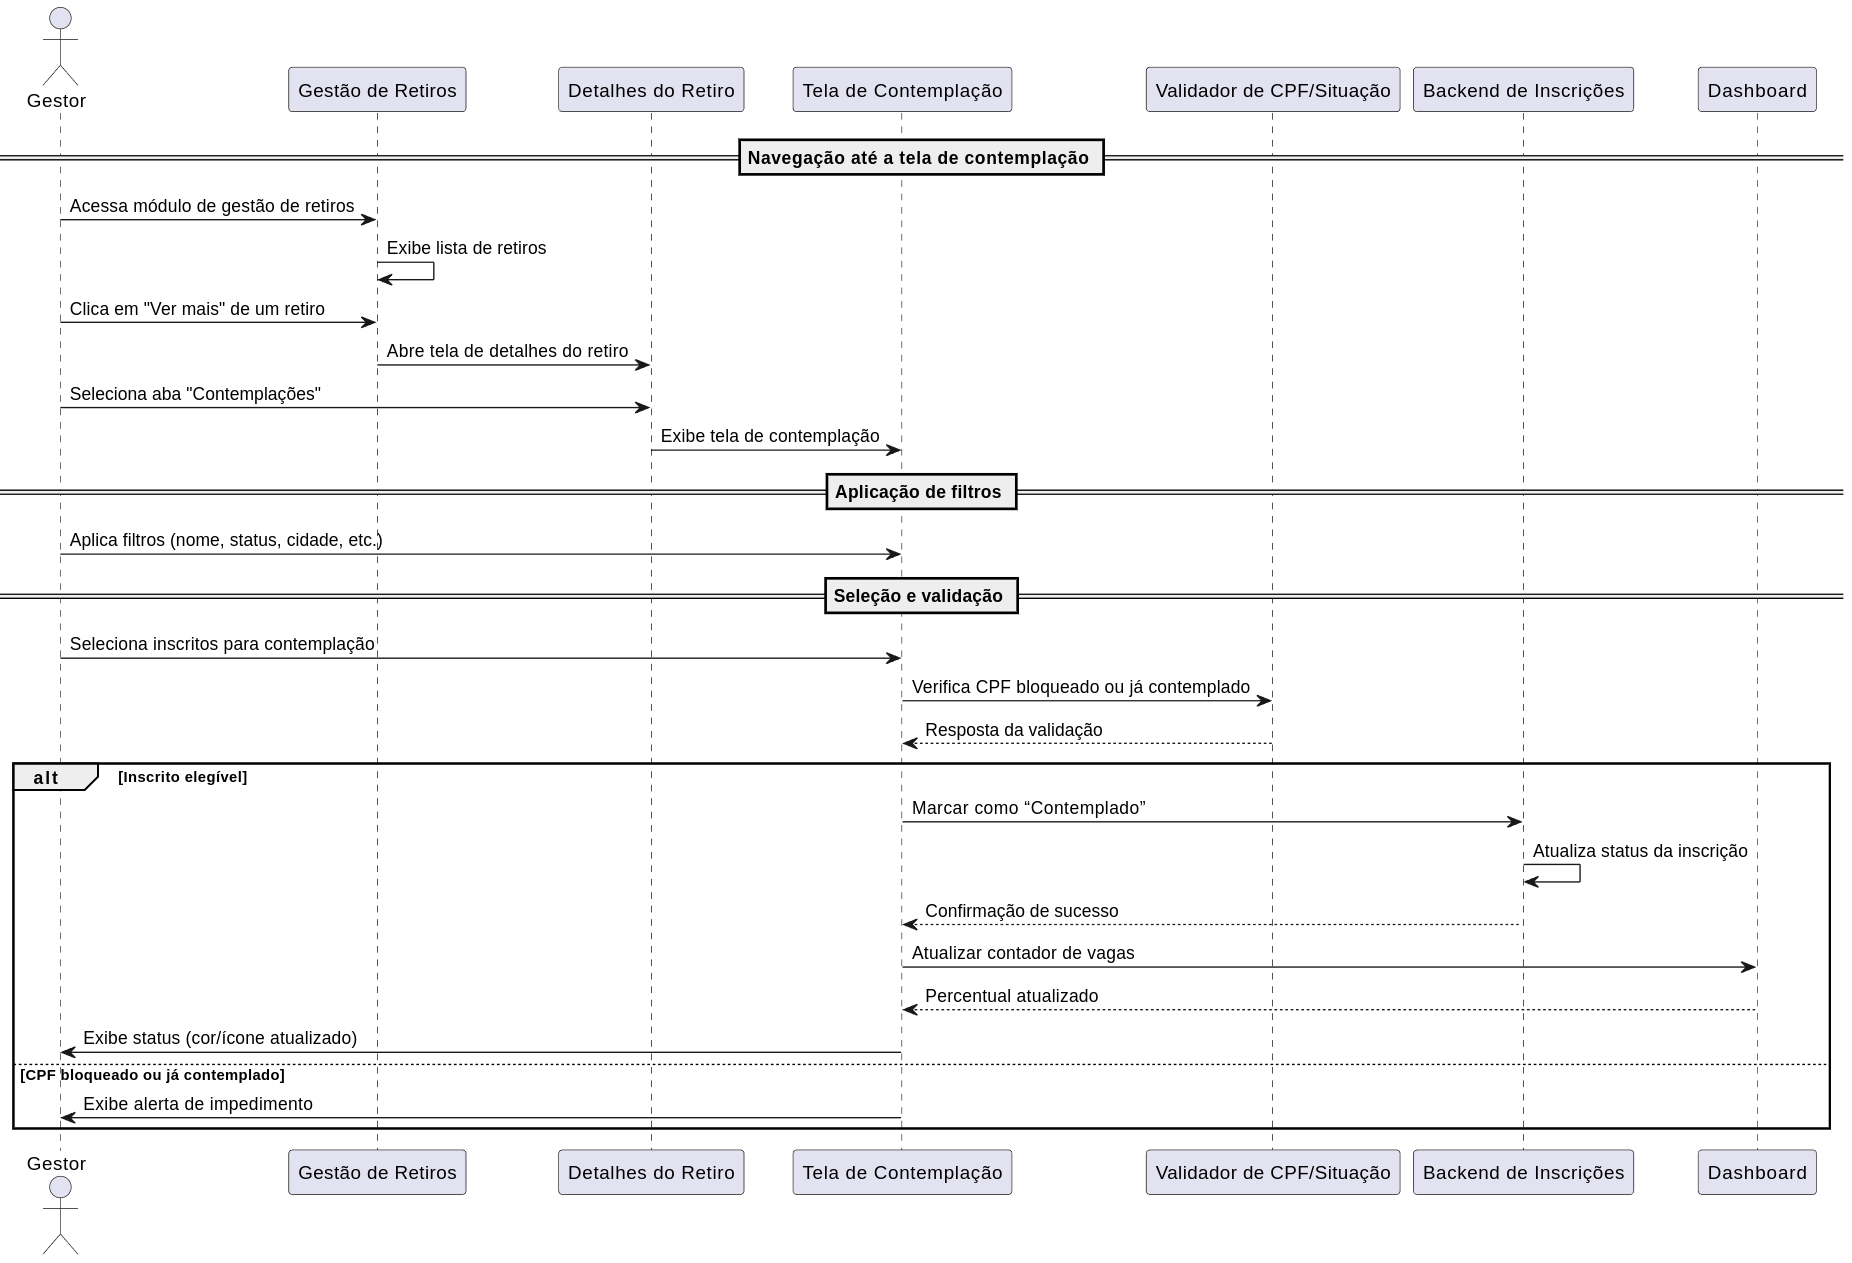
\includegraphics[width=0.9\textwidth]{images/diagramasdesequencias/manualParticipantSubscription.png}
    \caption{Diagrama de sequência para inscrição manual de participantes}
    \label{fig:manualParticipantInscription}
\end{figure}

O fluxo tem início com o gestor acessando o módulo de inscrições dentro do retiro selecionado. Ao optar por realizar o cadastro manual, o sistema apresenta o formulário interno com os mesmos campos do formulário público. Após o preenchimento, os dados são validados quanto à obrigatoriedade e à situação do CPF. Caso o CPF esteja bloqueado, o sistema retorna uma mensagem de erro. Se os dados forem válidos, a inscrição é armazenada e o gestor recebe a confirmação de sucesso.

Na alternativa de importação, o gestor seleciona um arquivo `.csv`. O sistema valida todas as linhas e separa aquelas com erro das válidas. As inscrições corretas são processadas em lote pelo backend, e ao final, é exibido um resumo com o número de registros bem-sucedidos e rejeitados.

\subsection{Diagrama de Sequência – Pagamento Manual via WhatsApp}

A Figura~\ref{fig:participantPayment} descreve o fluxo realizado pelo gestor ao confirmar manualmente o pagamento de um participante que enviou comprovante via WhatsApp. Esse processo inclui a navegação até o inscrito, edição do status de pagamento e envio do comprovante.

\begin{figure}[H]
    \centering
    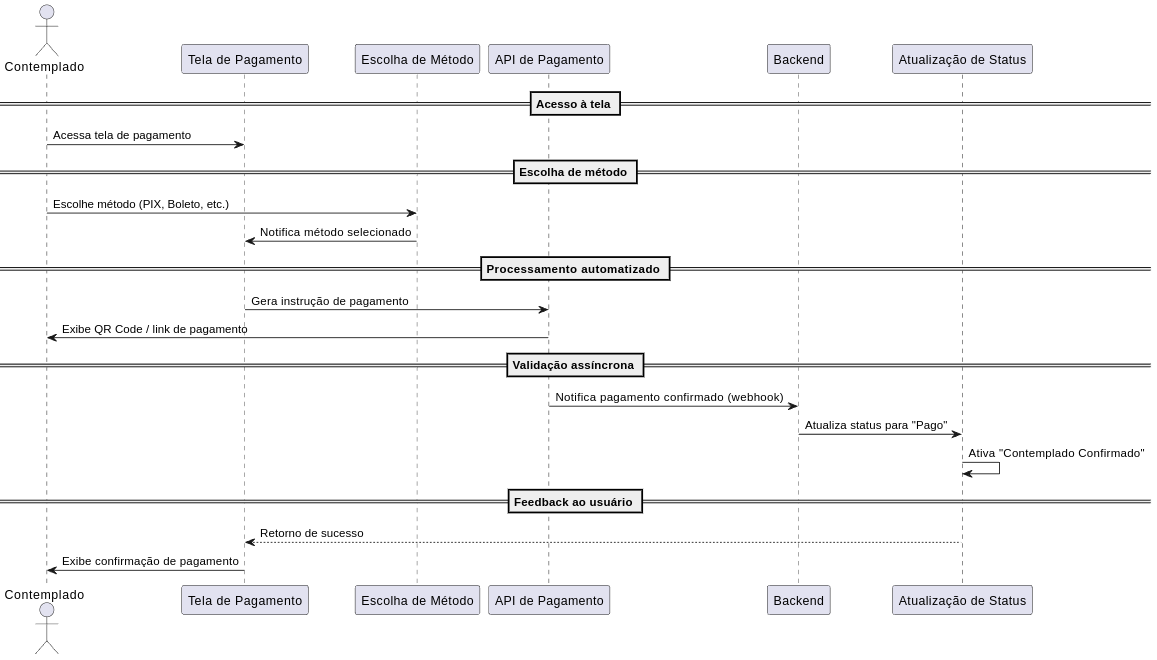
\includegraphics[width=0.9\textwidth]{images/diagramasdesequencias/participantPayment.png}
    \caption{Diagrama de sequência para confirmação manual de pagamento via WhatsApp}
    \label{fig:participantPayment}
\end{figure}

O fluxo se inicia com o gestor acessando os detalhes de um retiro e navegando até a aba “Contemplados”. Após localizar o inscrito, o gestor realiza um clique com o botão direito para abrir o menu de contexto e seleciona a opção “Editar Pagamento”. Um modal é exibido, permitindo ao gestor alterar o status de pagamento de “Pendente” para “Pago” e fazer upload do comprovante recebido (imagem ou PDF).

O sistema realiza a validação do arquivo enviado quanto ao tipo e tamanho. Caso esteja válido, a informação é enviada ao backend, que armazena o comprovante e atualiza o status do participante. Por fim, uma mensagem de confirmação é exibida e a lista de contemplados é atualizada com o novo status.

\subsection{Diagrama de Sequência – Envio de Mensagem de Contemplação}

\subsection{Diagrama de Sequência – Contemplação de Participantes}

A Figura~\ref{fig:participantContemplation} apresenta o fluxo realizado pelo gestor ao contemplar participantes inscritos em um retiro, incluindo etapas de filtro, validação de elegibilidade e atualização de status e indicadores.

\begin{figure}[H]
    \centering
    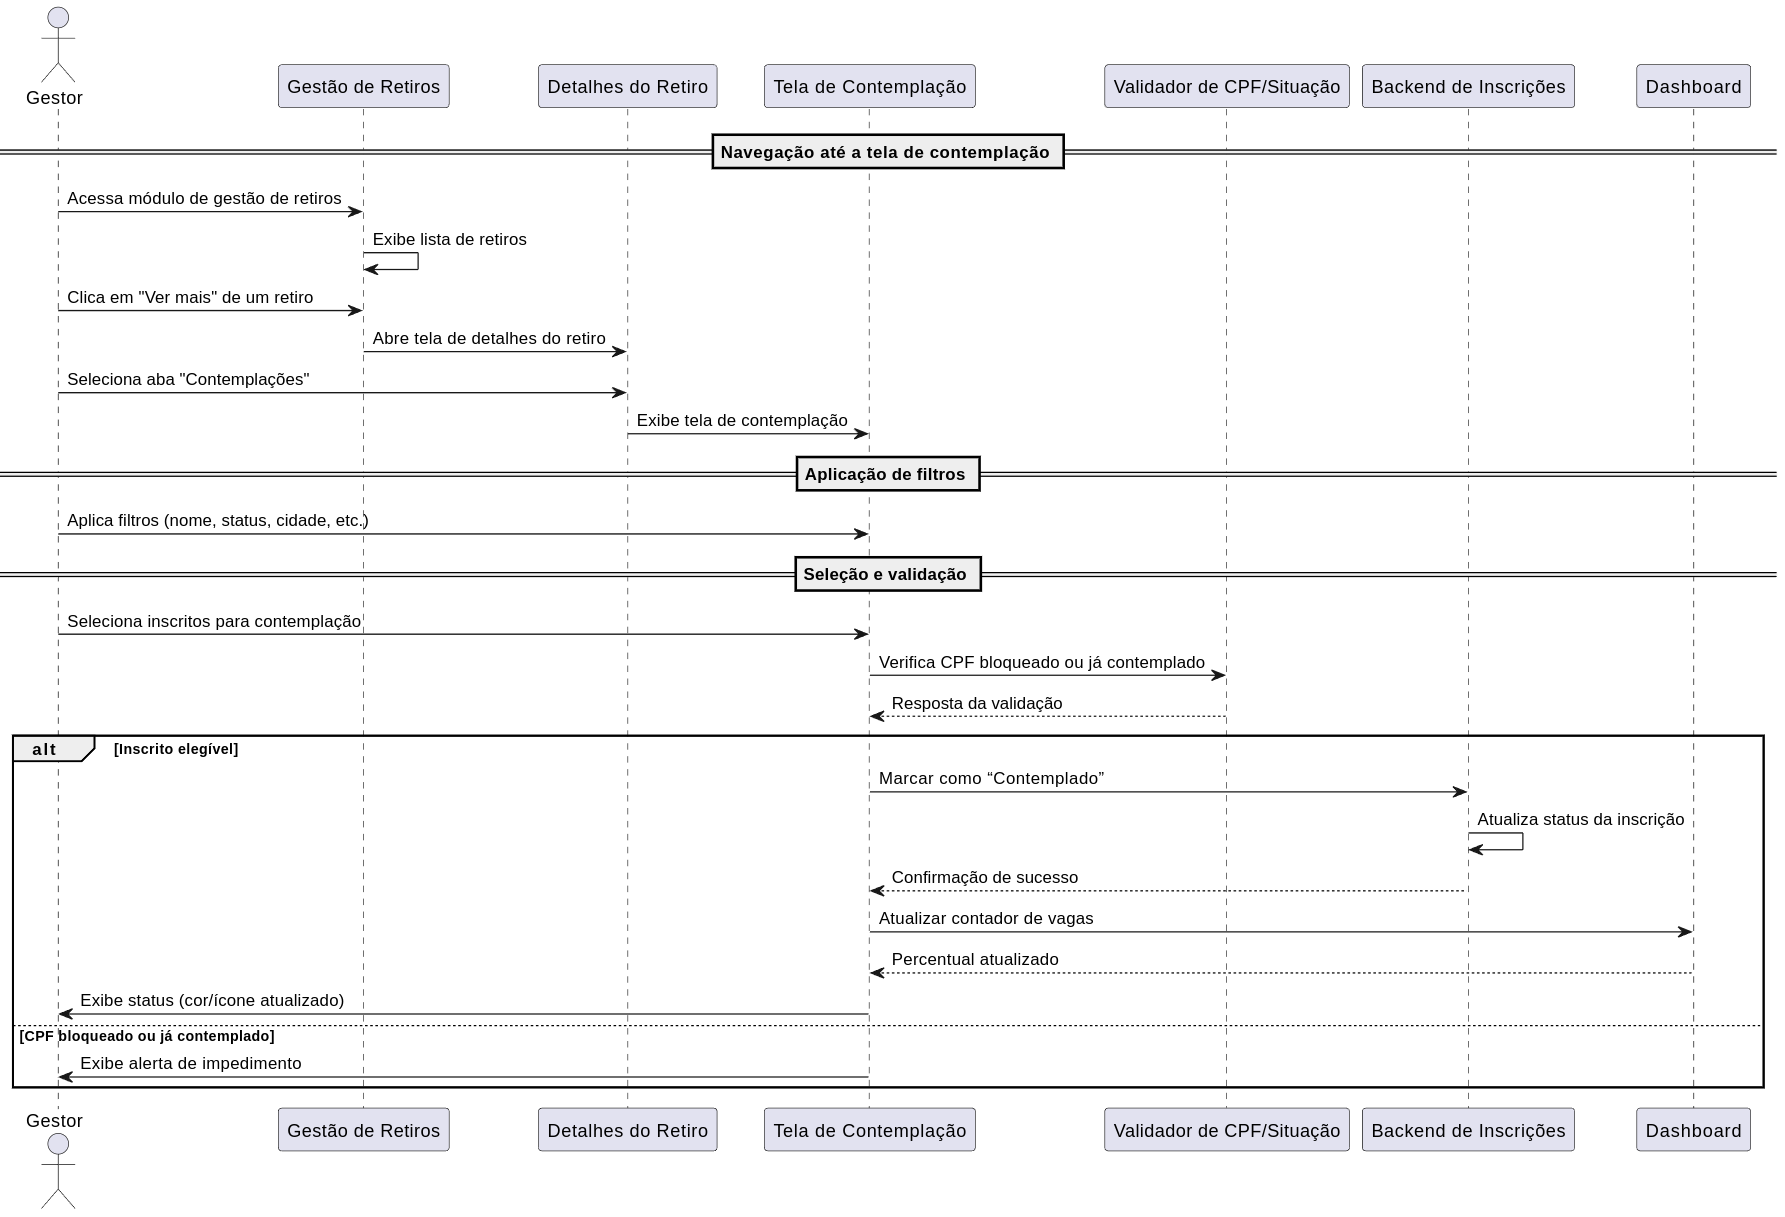
\includegraphics[width=0.9\textwidth]{images/diagramasdesequencias/participantContemplation.png}
    \caption{Diagrama de sequência para contemplação de participantes}
    \label{fig:participantContemplation}
\end{figure}

O processo se inicia quando o gestor acessa a área de gestão de retiros e, em seguida, a aba “Contemplações” de um retiro específico. Nessa tela, é possível aplicar filtros para facilitar a busca de participantes. Após selecionar os inscritos desejados, o sistema realiza uma verificação para validar se o CPF está bloqueado ou se o participante já foi contemplado.

Se o participante for elegível, o backend atualiza o status para “Contemplado” e o dashboard é atualizado para refletir o novo percentual de vagas ocupadas. O sistema então exibe o novo status visualmente ao gestor. Caso haja impedimentos, como CPF bloqueado ou contemplação anterior, o sistema alerta o gestor e impede a finalização da ação.


A Figura~\ref{fig:contemplationMessageSend} ilustra o fluxo realizado pelo gestor ao enviar mensagens personalizadas para os participantes contemplados, utilizando diferentes canais como WhatsApp e e-mail.

\begin{figure}[H]
    \centering
    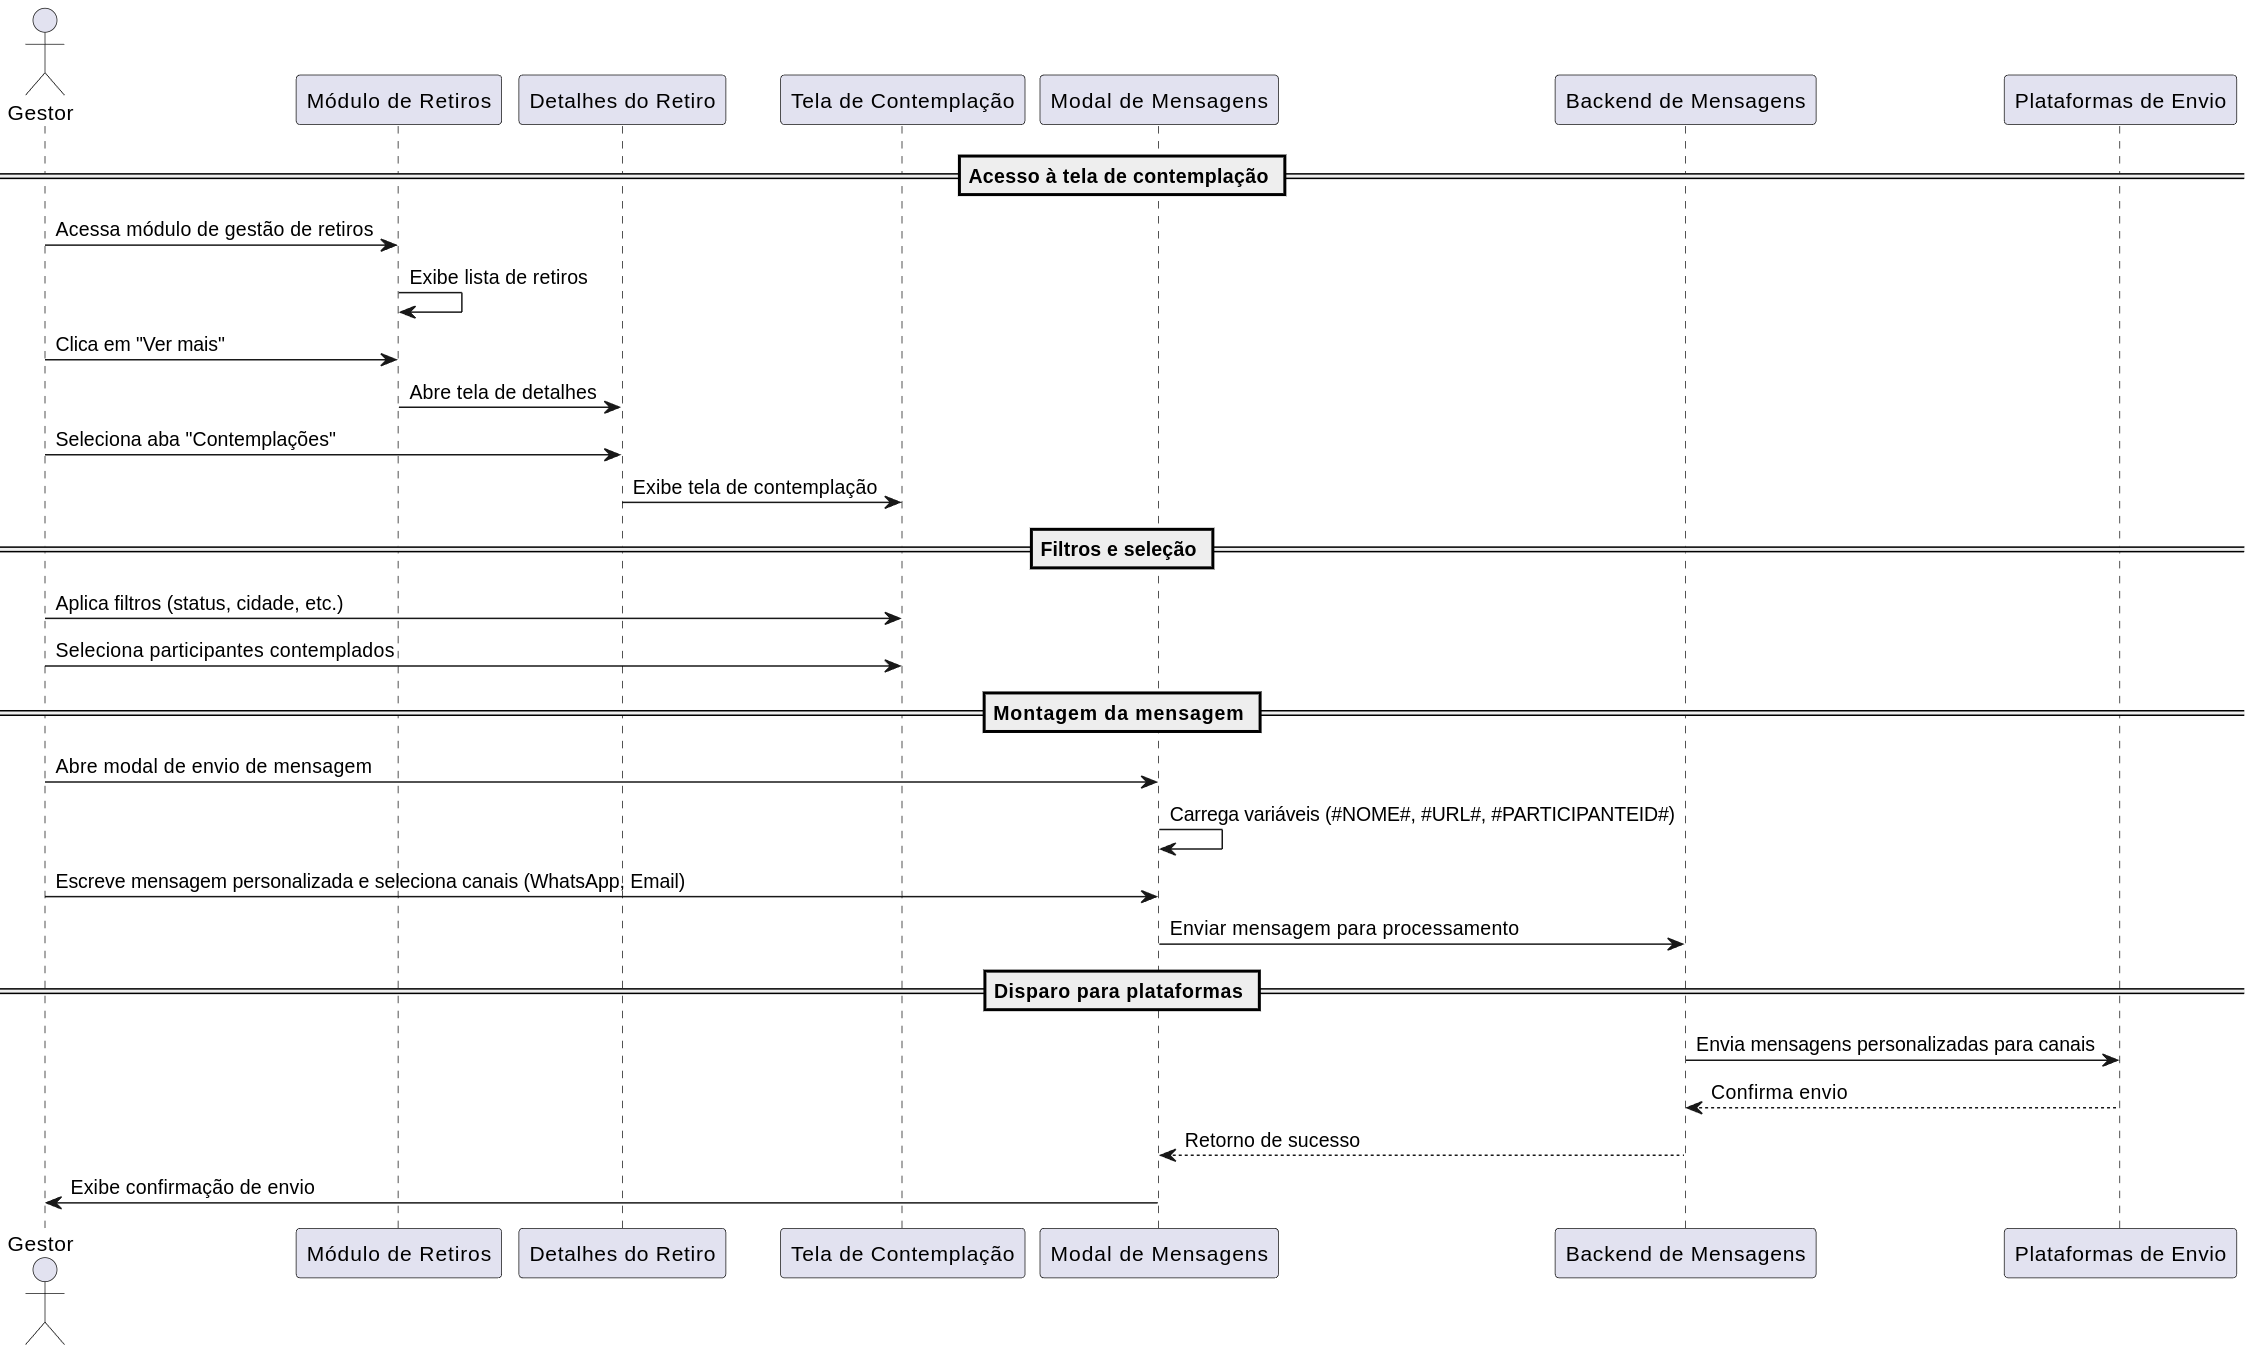
\includegraphics[width=0.9\textwidth]{images/diagramasdesequencias/manualContemplationMessage.png}
    \caption{Diagrama de sequência para envio de mensagem de contemplação}
    \label{fig:contemplationMessageSend}
\end{figure}

O fluxo se inicia com o gestor acessando o módulo de gestão de retiros e entrando na tela de detalhes de um retiro específico. Ao selecionar a aba “Contemplações”, é exibida a interface para aplicar filtros e selecionar os participantes que serão notificados.

Em seguida, o gestor abre o modal de mensagens, onde pode escrever o conteúdo da mensagem, utilizar variáveis como `\#NOME\#` e `\#URL\#`, e escolher os canais de envio. O backend de mensagens processa o conteúdo e o distribui para as plataformas responsáveis, como APIs de WhatsApp e serviços de e-mail. Após a confirmação do envio, o sistema exibe uma mensagem de sucesso ao gestor.

\subsection{Diagrama de Sequência – Processo de Pagamento Automatizado}

A Figura~\ref{fig:participantPaymentAuto} descreve o fluxo de pagamento automatizado realizado pelo participante contemplado, desde a escolha do método até a confirmação automática da transação via webhook.

\begin{figure}[H]
    \centering
    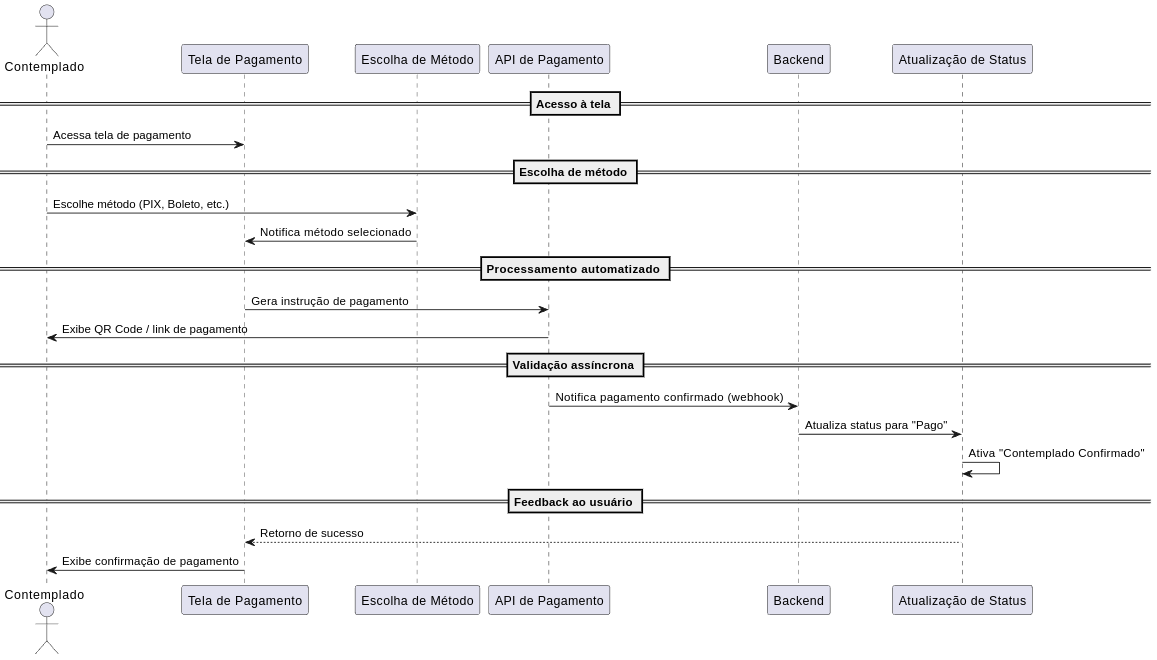
\includegraphics[width=0.9\textwidth]{images/diagramasdesequencias/participantPayment.png}
    \caption{Diagrama de sequência para processo de pagamento automatizado}
    \label{fig:participantPaymentAuto}
\end{figure}

O fluxo se inicia quando o participante contemplado acessa a tela de pagamento e seleciona o método desejado (como PIX ou boleto). O sistema, então, gera uma instrução de pagamento por meio de integração com uma API de pagamentos, que exibe ao usuário um QR Code ou link para realizar o pagamento.

Após o pagamento ser efetuado, a confirmação ocorre de forma assíncrona através de um webhook. A API de pagamentos notifica o backend, que atualiza o status da inscrição para “Pago” e ativa a confirmação da contemplação. Por fim, o sistema exibe ao usuário uma mensagem de confirmação com o status atualizado.

\subsection{Diagrama de Sequência – Composição Manual de Famílias}

A Figura~\ref{fig:familyManualComposition} descreve o fluxo de interação realizado pelo gestor ao compor manualmente as famílias do retiro, arrastando membros e validando regras de convivência, limite e diversidade.

\begin{figure}[H]
    \centering
    \includegraphics[width=0.9\textwidth]{images/diagramasdesequencias/familiyComposition.png}
    \caption{Diagrama de sequência para composição manual de famílias}
    \label{fig:familyManualComposition}
\end{figure}

O processo se inicia quando o gestor interage com a interface de composição e arrasta um membro para dentro de uma família. Imediatamente, o sistema realiza validações em tempo real para verificar se há violação de regras como o limite máximo de membros por família, conflito de parentesco, proporção de gênero e presença de padrinhos ou madrinhas.

Caso alguma regra seja violada, um alerta visual é exibido ao gestor. Caso contrário, a nova composição é enviada ao backend para persistência. O sistema então atualiza os dados e apresenta estatísticas atualizadas, como proporções de gênero e quantidade de padrinhos na família.

\subsection{Diagrama de Sequência – Sorteio Automático de Famílias}

A Figura~\ref{fig:familyAutoDraw} apresenta o fluxo realizado pelo gestor ao acionar a funcionalidade de sorteio automático para composição das famílias, com validação de regras e exibição de feedback visual.

\begin{figure}[H]
    \centering
    \includegraphics[width=0.9\textwidth]{images/diagramasdesequencias/familyDraw.png}
    \caption{Diagrama de sequência para sorteio automático de famílias}
    \label{fig:familyAutoDraw}
\end{figure}

O processo se inicia quando o gestor clica no botão “SORTEAR” na tela de composição de famílias. O sistema solicita ao backend a geração aleatória de famílias, que realiza a distribuição dos participantes conforme regras internas. Em seguida, um validador verifica possíveis conflitos, como membros da mesma família biológica sendo alocados juntos indevidamente.

Se forem encontrados conflitos, o sistema alerta o gestor para que ajustes manuais sejam realizados. Caso contrário, a nova composição é exibida automaticamente na interface, acompanhada de uma mensagem de sucesso e atualização visual da estrutura familiar.

\subsection{Diagrama de Sequência – Cadastro de Famílias}

A Figura~\ref{fig:familyCreate} apresenta o fluxo realizado pelo gestor ao cadastrar uma nova família no sistema, vinculando-a a um retiro específico.

\begin{figure}[H]
    \centering
    \includegraphics[width=0.9\textwidth]{images/diagramasdesequencias/familyRegister.png}
    \caption{Diagrama de sequência para cadastro de famílias}
    \label{fig:familyCreate}
\end{figure}

O processo tem início quando o gestor acessa o módulo de famílias e clica na opção “Nova Família”. Em seguida, o sistema exibe um formulário no qual o gestor deve preencher o nome da família, a quantidade máxima de membros e o retiro ao qual ela será vinculada.

Após o preenchimento, o sistema valida os campos obrigatórios. Se houver erros, como ausência do nome ou do retiro, uma mensagem de erro é exibida. Caso os dados estejam corretos, o backend realiza o armazenamento no banco de dados e retorna uma confirmação de sucesso. A interface é então atualizada, exibindo a nova família na lista.

\subsection{Diagrama de Sequência – Criação de Grupos de WhatsApp por Família}

A Figura~\ref{fig:familyWhatsappGroup} apresenta o fluxo realizado pelo gestor ao acionar a funcionalidade de criação automática de grupos de WhatsApp para as famílias cadastradas no retiro.

\begin{figure}[H]
    \centering
    \includegraphics[width=0.9\textwidth]{images/diagramasdesequencias/familyWpGroup.png}
    \caption{Diagrama de sequência para criação de grupos de WhatsApp por família}
    \label{fig:familyWhatsappGroup}
\end{figure}

O processo é iniciado quando o gestor acessa a tela de famílias e clica no botão “Criar Grupos de WhatsApp”. O sistema então aciona o backend de comunicação, que se comunica com a API do WhatsApp para criar os grupos automaticamente, um para cada família registrada.

Durante o processo, o backend recebe o status individual de cada operação, como criação do grupo, adição dos membros e possíveis falhas. Ao final, um relatório de status é exibido ao gestor, informando os resultados para cada família — incluindo sucesso, falhas ou ausência de membros vinculados.

\subsection{Diagrama de Sequência – Atribuição de Funções na Equipe de Serviço}

A Figura~\ref{fig:teamRoleAssign} apresenta o fluxo realizado pelo gestor ao atribuir funções específicas (como Coordenador, Vice ou Membro) aos participantes de uma equipe de serviço.

\begin{figure}[H]
    \centering
    \includegraphics[width=0.9\textwidth]{images/diagramasdesequencias/teamAtribuition.png}
    \caption{Diagrama de sequência para atribuição de funções na equipe de serviço}
    \label{fig:teamRoleAssign}
\end{figure}

O processo se inicia quando o gestor acessa uma equipe existente na tela de equipes e seleciona um dos participantes para definir sua função. O sistema verifica se as regras específicas da composição da equipe estão sendo respeitadas, como a limitação de apenas um coordenador por equipe.

Se alguma regra for violada, é exibido um alerta visual com o motivo do impedimento. Caso contrário, a nova função é enviada ao backend para ser salva, e uma confirmação de sucesso é apresentada ao gestor.

\subsection{Diagrama de Sequência – Cadastro de Equipe de Serviço}

A Figura~\ref{fig:teamCreate} apresenta o fluxo realizado pelo gestor ao cadastrar uma nova equipe de serviço, utilizando um formulário manual ou com base em um modelo pré-cadastrado.

\begin{figure}[H]
    \centering
    \includegraphics[width=0.9\textwidth]{images/diagramasdesequencias/teamCreate.png}
    \caption{Diagrama de sequência para cadastro de equipe de serviço}
    \label{fig:teamCreate}
\end{figure}

O processo tem início com o gestor acessando o módulo de equipes e clicando em “Nova Equipe” ou selecionando um modelo existente. O sistema apresenta um formulário para preenchimento de informações como nome, descrição, número mínimo e máximo de membros, e seleção de coordenador e vice.

Após o preenchimento, os campos obrigatórios são validados. Caso haja erros, o sistema exibe uma mensagem orientando a correção. Se os dados estiverem corretos, o backend realiza o armazenamento da equipe e retorna uma confirmação, que é então exibida ao gestor.

\subsection{Diagrama de Sequência – Distribuição de Membros nas Equipes}

A Figura~\ref{fig:teamDistribution} descreve o processo de movimentação de membros entre equipes de serviço, respeitando os limites máximos de alocação definidos para cada equipe.

\begin{figure}[H]
    \centering
    \includegraphics[width=0.9\textwidth]{images/diagramasdesequencias/teamDistribution.png}
    \caption{Diagrama de sequência para distribuição de membros nas equipes}
    \label{fig:teamDistribution}
\end{figure}

O fluxo se inicia quando o gestor interage com a tela de equipes e move um membro de uma equipe para outra, seja por arraste (drag \texttt{\&} drop) ou por seleção direta. O sistema valida se a equipe de destino ainda possui vagas disponíveis.

Caso o limite máximo de membros já tenha sido atingido, um aviso é exibido ao gestor informando que a equipe está cheia. Caso contrário, a nova alocação é enviada ao backend, que persiste a alteração e retorna uma confirmação. A interface é então atualizada com a nova contagem de membros e vagas disponíveis.

\subsection{Diagrama de Sequência – Cadastro de Barracas}

A Figura~\ref{fig:tentCreate} apresenta o fluxo de cadastro de barracas realizado pelo gestor, tanto de forma individual quanto por meio da funcionalidade de cadastro em lote.

\begin{figure}[H]
    \centering
    \includegraphics[width=0.9\textwidth]{images/diagramasdesequencias/tentCreation.png}
    \caption{Diagrama de sequência para cadastro de barracas}
    \label{fig:tentCreate}
\end{figure}

No modo de cadastro individual, o gestor clica em “Nova Barraca” e preenche informações como número, capacidade, categoria e observações. O sistema valida os campos obrigatórios e, se estiverem corretos, envia os dados para o backend, que realiza o armazenamento e retorna uma mensagem de sucesso.

No modo de cadastro em lote, o gestor informa uma faixa numérica (por exemplo, de 1 a 50) e a categoria das barracas. O sistema valida o intervalo e, se for válido, gera automaticamente as barracas correspondentes e realiza a persistência em lote. Ao final, uma mensagem de confirmação com o total de barracas cadastradas é exibida ao gestor.

\subsection{Diagrama de Sequência – Atribuição de Participante à Barraca}

A Figura~\ref{fig:tentAssign} descreve o fluxo realizado pelo gestor ao alocar manualmente um participante em uma barraca, verificando automaticamente a disponibilidade da mesma.

\begin{figure}[H]
    \centering
    \includegraphics[width=0.9\textwidth]{images/diagramasdesequencias/tentaddParticipant.png}
    \caption{Diagrama de sequência para atribuição de participante à barraca}
    \label{fig:tentAssign}
\end{figure}

O fluxo se inicia quando o gestor seleciona um participante e escolhe uma barraca de destino na interface de acomodações. O sistema valida a lotação da barraca, consultando o backend para obter a quantidade atual de ocupantes.

Se a barraca já estiver cheia, o sistema exibe um aviso visual informando a indisponibilidade. Caso contrário, o vínculo entre participante e barraca é atualizado no backend e a interface é atualizada com a nova alocação, refletindo visualmente a ocupação da barraca.

\subsection{Diagrama de Sequência – Inscrição Pública}

A Figura~\ref{fig:publicInscription} apresenta o fluxo realizado por um visitante ao acessar o formulário público de inscrição para um retiro e realizar sua candidatura.

\begin{figure}[H]
    \centering
    \includegraphics[width=0.9\textwidth]{images/diagramasdesequencias/participantFormSubscription.png}
    \caption{Diagrama de sequência para inscrição pública}
    \label{fig:publicInscription}
\end{figure}

O fluxo se inicia com o visitante acessando o link público de inscrição. Ao preencher os dados solicitados, como nome e CPF, o sistema realiza a validação do CPF e da data de nascimento, incluindo verificações contra bloqueios.

Caso o período de inscrições esteja encerrado, o sistema exibe uma mensagem apropriada. Se a inscrição for válida, os dados são enviados ao backend, que os processa e armazena. Por fim, uma confirmação de sucesso é exibida ao visitante.


\subsection{Diagrama de Sequência – Recebimento da Mensagem e Acesso ao Sistema}

A Figura~\ref{fig:participantAccess} apresenta o fluxo realizado pelo participante contemplado ao receber a mensagem de confirmação e acessar o sistema por meio de um link personalizado.

\begin{figure}[H]
    \centering
    \includegraphics[width=0.9\textwidth]{images/diagramasdesequencias/manualContemplationMessage.png}
    \caption{Diagrama de sequência para recebimento da mensagem e acesso ao sistema}
    \label{fig:participantAccess}
\end{figure}

O fluxo se inicia com o envio da mensagem contendo o link de acesso individualizado, que é recebido pelo participante contemplado. Ao clicar nesse link, ele é redirecionado para a tela de cadastro, já contendo seu identificador (`ContempladoID`) de forma embutida.

Na tela de cadastro, o participante preenche os dados solicitados e confirma. O backend valida e armazena as informações, retornando sucesso. Em seguida, o sistema redireciona automaticamente o usuário para a tela inicial, que contém seus dados pessoais, informações sobre o retiro para o qual foi contemplado e a área de pagamento.

\subsection{Diagrama de Sequência – Processo de Pagamento Automatizado (Versão Atualizada)}

A Figura~\ref{fig:participantPaymentAutoV2} descreve o fluxo realizado pelo participante ao efetuar um pagamento via sistema integrado, com atualização imediata do status para "Pagamento Pendente" após a escolha do método, e confirmação automática via webhook.

\begin{figure}[H]
    \centering
    \includegraphics[width=0.9\textwidth]{images/diagramasdesequencias/participantPayment.png}
    \caption{Diagrama de sequência para processo de pagamento automatizado com status pendente}
    \label{fig:participantPaymentAutoV2}
\end{figure}

O fluxo se inicia com o acesso do participante à tela de pagamento, onde ele escolhe o método desejado (como PIX ou Boleto). Após a seleção, o sistema registra o status como “Pagamento Pendente” e gera a instrução de pagamento via integração com a API de pagamentos, que fornece um QR Code ou link para efetivação.

O pagamento é confirmado de forma assíncrona, por meio de um webhook da API de pagamentos para o backend. Após o recebimento dessa confirmação, o status da inscrição é atualizado para “Pago” e o sistema marca o participante como “Confirmado”. Por fim, o participante recebe o feedback de sucesso com a confirmação visual da operação.

\subsection{Diagrama de Sequência – Geração de Relatório}

A Figura~\ref{fig:reportGeneration} apresenta o fluxo realizado pelo gestor ao gerar relatórios com base em filtros definidos, permitindo tanto a visualização em tela quanto a exportação para PDF ou CSV.

\begin{figure}[H]
    \centering
    \includegraphics[width=0.9\textwidth]{images/diagramasdesequencias/report.png}
    \caption{Diagrama de sequência para geração de relatório}
    \label{fig:reportGeneration}
\end{figure}

O processo inicia-se quando o gestor acessa o módulo de relatórios e seleciona o tipo de relatório desejado. Em seguida, o sistema exibe os filtros disponíveis, como data, status ou outras informações relevantes. Após configurar os filtros, o sistema consulta o backend, que realiza uma busca no banco de dados e retorna os dados correspondentes.

Esses dados são renderizados em uma tabela visual na interface. Caso o gestor opte por exportar os resultados, o sistema aciona o gerador de arquivos (PDF ou CSV), que formata e retorna o arquivo para download. Se não houver exportação, a visualização permanece apenas em tela.

\subsection{Diagrama de Sequência – Notificações}

A Figura~\ref{fig:notificationFlow} apresenta o fluxo de funcionamento do sistema de notificações, desde o carregamento das mensagens até a navegação para o conteúdo relacionado à notificação selecionada.

\begin{figure}[H]
    \centering
    \includegraphics[width=0.9\textwidth]{images/diagramasdesequencias/notification.png}
    \caption{Diagrama de sequência para recebimento e interação com notificações}
    \label{fig:notificationFlow}
\end{figure}

O fluxo se inicia quando o usuário acessa o sistema. Neste momento, o sistema solicita ao módulo de notificações as mensagens destinadas ao usuário. A lista de notificações é retornada e exibida de forma resumida na interface.

Ao interagir com uma notificação (clicando em “Ver mais”), o sistema solicita ao módulo de notificações os detalhes da mensagem, incluindo o destino associado. O usuário é então redirecionado para o módulo correspondente, onde poderá visualizar o conteúdo relacionado à notificação.


%cronograma
\chapter{CRONOGRAMA}

\begin{table}[H]
\centering
\caption{Cronograma de Desenvolvimento do Projeto}
\begin{tabular}{|p{7cm}|c|c|c|c|c|c|c|c|}
\hline
\textbf{Etapas} & \textbf{Abr} & \textbf{Mai} & \textbf{Jun} & \textbf{Jul} & \textbf{Ago} & \textbf{Set} & \textbf{Out} & \textbf{Nov} \\
\hline
Levantamento de requisitos e análise do problema & X & X &   &   &   &   &   &   \\
\hline
Estudos teóricos e fundamentação & X & X & X &   &   &   &   &   \\
\hline
Prototipação de telas e fluxos (Figma) &   & X & X &   &   &   &   &   \\
\hline
Planejamento da arquitetura front-end &   &   & X & X &   &   &   &   \\
\hline
Desenvolvimento da interface (UI + lógica) &   &   &   & X & X & X &   &   \\
\hline
Integração com API e testes funcionais &   &   &   &   & X & X & X &   \\
\hline
Refinamento da experiência do usuário (UX) &   &   &   &   &   & X & X &   \\
\hline
Documentação e redação final do TCC &   &   &   &   &   &   & X & X \\
\hline
Apresentação e entrega final &   &   &   &   &   &   &   & X \\
\hline
\end{tabular}
\label{tab:cronograma}
\end{table}


%CONCLUSÃO
\include{conteudo/https://www.figma.com/design/d41tmdruHYmRqwj2LL2lOB/Servo-Fiel---TCC-BCC-2H25?node-id=17-20&t=W3T09fJeqrwljeok-1}

% ----------------------------------------------------------
% ELEMENTOS PÓS-TEXTUAIS
% ----------------------------------------------------------
\postextual

% ----------------------------------------------------------
% Referências bibliográficas
% ----------------------------------------------------------

\bibliography{referencias}

%Apêndices

\appendix
\chapter*{Anexo A - Protótipo da Interface no Figma}
\addcontentsline{toc}{chapter}{Anexo A - Protótipo da Interface no Figma}

O protótipo interativo do sistema SAMGestor pode ser acessado por meio do seguinte link:

\url{https://www.figma.com/design/d41tmdruHYmRqwj2LL2lOB/Servo-Fiel---TCC-BCC-2H25?node-id=17-20&t=W3T09fJeqrwljeok-1}


%Anexos
% \begin{anexosenv}
% \chapter{Título do Anexo A}
% \label{anexoA}

% Arquivos não confeccionados pelo autor do trabalho.


% \end{anexosenv}


%---------------------------------------------------------------------
% INDICE REMISSIVO
%---------------------------------------------------------------------
% \printindex
\end{document}